% Options for packages loaded elsewhere
% Options for packages loaded elsewhere
\PassOptionsToPackage{unicode}{hyperref}
\PassOptionsToPackage{hyphens}{url}
\PassOptionsToPackage{dvipsnames,svgnames,x11names}{xcolor}
%
\documentclass[
  10pt,
  a4paper,
  DIV=11,
  numbers=noendperiod,
  open=any]{scrreprt}
\usepackage{xcolor}
\usepackage[margin=2cm]{geometry}
\usepackage{amsmath,amssymb}
\usepackage[spanish]{babel}
\usepackage{hyperref}
\usepackage{fontawesome5}
\usepackage{mathtools}
\setcounter{secnumdepth}{5}
\usepackage{iftex}
\ifPDFTeX
  \usepackage[T1]{fontenc}
  \usepackage[utf8]{inputenc}
  \usepackage{textcomp} % provide euro and other symbols
\else % if luatex or xetex
  \usepackage{unicode-math} % this also loads fontspec
  \defaultfontfeatures{Scale=MatchLowercase}
  \defaultfontfeatures[\rmfamily]{Ligatures=TeX,Scale=1}
\fi
\usepackage{lmodern}
\ifPDFTeX\else
  % xetex/luatex font selection
\fi
% Use upquote if available, for straight quotes in verbatim environments
\IfFileExists{upquote.sty}{\usepackage{upquote}}{}
\IfFileExists{microtype.sty}{% use microtype if available
  \usepackage[]{microtype}
  \UseMicrotypeSet[protrusion]{basicmath} % disable protrusion for tt fonts
}{}
\makeatletter
\@ifundefined{KOMAClassName}{% if non-KOMA class
  \IfFileExists{parskip.sty}{%
    \usepackage{parskip}
  }{% else
    \setlength{\parindent}{0pt}
    \setlength{\parskip}{6pt plus 2pt minus 1pt}}
}{% if KOMA class
  \KOMAoptions{parskip=half}}
\makeatother
% Make \paragraph and \subparagraph free-standing
\makeatletter
\ifx\paragraph\undefined\else
  \let\oldparagraph\paragraph
  \renewcommand{\paragraph}{
    \@ifstar
      \xxxParagraphStar
      \xxxParagraphNoStar
  }
  \newcommand{\xxxParagraphStar}[1]{\oldparagraph*{#1}\mbox{}}
  \newcommand{\xxxParagraphNoStar}[1]{\oldparagraph{#1}\mbox{}}
\fi
\ifx\subparagraph\undefined\else
  \let\oldsubparagraph\subparagraph
  \renewcommand{\subparagraph}{
    \@ifstar
      \xxxSubParagraphStar
      \xxxSubParagraphNoStar
  }
  \newcommand{\xxxSubParagraphStar}[1]{\oldsubparagraph*{#1}\mbox{}}
  \newcommand{\xxxSubParagraphNoStar}[1]{\oldsubparagraph{#1}\mbox{}}
\fi
\makeatother


\usepackage{longtable,booktabs,array}
\usepackage{calc} % for calculating minipage widths
% Correct order of tables after \paragraph or \subparagraph
\usepackage{caption}
\usepackage{etoolbox}
\AtBeginEnvironment{figure}{\centering}
\captionsetup{justification=centering,singlelinecheck=false}

\makeatletter
\patchcmd\longtable{\par}{\if@noskipsec\mbox{}\fi\par}{}{}
\makeatother
% Allow footnotes in longtable head/foot
\IfFileExists{footnotehyper.sty}{\usepackage{footnotehyper}}{\usepackage{footnote}}
\makesavenoteenv{longtable}
\usepackage{graphicx}
\makeatletter
\newsavebox\pandoc@box
\newcommand*\pandocbounded[1]{% scales image to fit in text height/width
  \sbox\pandoc@box{#1}%
  \Gscale@div\@tempa{\textheight}{\dimexpr\ht\pandoc@box+\dp\pandoc@box\relax}%
  \Gscale@div\@tempb{\linewidth}{\wd\pandoc@box}%
  \ifdim\@tempb\p@<\@tempa\p@\let\@tempa\@tempb\fi% select the smaller of both
  \ifdim\@tempa\p@<\p@\scalebox{\@tempa}{\usebox\pandoc@box}%
  \else\usebox{\pandoc@box}%
  \fi%
}
% Set default figure placement to htbp
\def\fps@figure{htbp}
\makeatother

\ifLuaTeX
  \usepackage{luacolor}
  \usepackage[soul]{lua-ul}
\else
  \usepackage{soul}
\fi




\setlength{\emergencystretch}{3em} % prevent overfull lines

\providecommand{\tightlist}{%
  \setlength{\itemsep}{0pt}\setlength{\parskip}{0pt}}



 


% ====== COLORES Y TIPOS DE TÍTULO (KOMA nativo) ======
\usepackage{xcolor}
\definecolor{Main}{HTML}{0F766E}     % verde azulado
\definecolor{Accent}{HTML}{2563EB}   % azul acento

% Tipos para cada nivel KOMA
\setkomafont{part}{\normalfont\bfseries\Huge\color{Main}}
\setkomafont{chapter}{\normalfont\bfseries\Huge\color{Main}}
\setkomafont{section}{\normalfont\bfseries\Large\color{Main}}
\setkomafont{subsection}{\normalfont\bfseries\large\color{Accent}}
\setkomafont{subsubsection}{\normalfont\bfseries\normalsize\color{Accent}}

% Espaciados de títulos (más seguros con nuestra cabecera)
\RedeclareSectionCommand[
  beforeskip=-2.0ex plus -1ex minus -.2ex,
  afterskip=2.0ex plus .5ex
]{chapter}
\RedeclareSectionCommand[
  beforeskip=-1.5ex plus -.7ex minus -.2ex,
  afterskip=1.0ex plus .3ex
]{section}
\RedeclareSectionCommand[
  beforeskip=-1.0ex plus -.5ex minus -.2ex,
  afterskip=.8ex plus .2ex
]{subsection}

% ====== CABECERA DE CAPÍTULO (franja superior + regla bajo título) ======
\usepackage{etoolbox} % <— nuevo, para ifstrempty

% ====== CABECERA DE CAPÍTULO (franja superior + regla bajo título) ======
\usepackage{tikz}
\newcommand*\ChapterDecor{%
  \begin{tikzpicture}[remember picture,overlay]
    \fill[Main] (current page.north west) rectangle ([yshift=-1.2cm]current page.north east);
  \end{tikzpicture}%
}

% Mantengo tu formato de número
%\renewcommand*\chapterformat{{\Large\bfseries\color{Main}\thechapter}\enskip}
\renewcommand*\chapterformat{%
  {\fontsize{38}{40}\selectfont\bfseries\color{Main}\thechapter}\enskip
}
% Imprime título con o sin número (no número en capítulos * como ToC)
\renewcommand*\chapterlinesformat[3]{%
  \ChapterDecor%
  \vspace*{1.4cm}%
  {\raggedright
   {\Huge\bfseries\color{Main}%
    \ifstrempty{#2}{}{#2\enskip}% #2 vacío => capítulo sin numerar (no imprimir número)
    #3\par}
   \vspace{.25cm}
   {\color{Main}\rule{\textwidth}{1.2pt}}
  }%
  \par\vspace{1.2ex}%
}


% ====== ENCABEZADOS Y PIES (KOMA: scrlayer-scrpage) ======
\usepackage[automark]{scrlayer-scrpage}
\clearpairofpagestyles
\ohead{\headmark}
\cfoot{\pagemark}
\setkomafont{pagehead}{\normalfont\itshape\color{gray!60}}
\setkomafont{pagenumber}{\normalfont\bfseries\color{gray!70}}

% ====== FIGURAS: ajuste global y enlaces clicables ======
\usepackage{graphicx}
\setkeys{Gin}{width=.8\linewidth,height=7cm,keepaspectratio}
\usepackage{hyperref}
\hypersetup{
  colorlinks=true,
  linkcolor=Accent,
  citecolor=Accent,
  urlcolor=Accent
}

% ====== PAQUETES DE MATEMÁTICAS ======
\usepackage{amsthm,amsmath,amssymb}
\usepackage{scrhack}
%\everydisplay{\tag{\thechapter.\arabic{equation}}\stepcounter{equation}}

% ====== COMPATIBILIDAD con comandos antiguos (\rm, \bf, \it, \tt, \sc) ======
\makeatletter
\DeclareOldFontCommand{\rm}{\normalfont\rmfamily}{\mathrm}
\DeclareOldFontCommand{\bf}{\normalfont\bfseries}{\mathbf}
\DeclareOldFontCommand{\it}{\normalfont\itshape}{\mathit}
\DeclareOldFontCommand{\tt}{\normalfont\ttfamily}{\mathtt}
\DeclareOldFontCommand{\sc}{\normalfont\scshape}{\@nomath\sc}
\makeatother

% ====== NUMERACIÓN POR CAPÍTULO ======
\usepackage{chngcntr}
\numberwithin{equation}{chapter}
\counterwithin{figure}{chapter}
\counterwithin{table}{chapter}

% ====== REFERENCIAS ======
\usepackage[nameinlink,capitalise]{cleveref}

% ====== UNICODE ÚTIL EN TEXTO ======
\usepackage{newunicodechar}
\newunicodechar{⇒}{\ensuremath{\Rightarrow}}
\newunicodechar{≥}{\ensuremath{\ge}}
\newunicodechar{𝛿}{\ensuremath{\delta}}
\newunicodechar{𝜃}{\ensuremath{\theta}}

% ====== ECUACIONES LARGAS ======
\allowdisplaybreaks

\usepackage{etoolbox}
\makeatletter
\g@addto@macro\@floatboxreset\centering
\makeatother

\renewcommand{\contentsname}{Tabla de contenidos}
\KOMAoption{captions}{tableheading}
\makeatletter
\@ifpackageloaded{caption}{}{\usepackage{caption}}

\AtBeginDocument{%
\ifdefined\contentsname
  \renewcommand*\contentsname{Table of contents}
\else
  \newcommand\contentsname{Table of contents}
\fi
\ifdefined\listfigurename
  \renewcommand*\listfigurename{List of Figures}
\else
  \newcommand\listfigurename{List of Figures}
\fi
\ifdefined\listtablename
  \renewcommand*\listtablename{List of Tables}
\else
  \newcommand\listtablename{List of Tables}
\fi
\ifdefined\figurename
  \renewcommand*\figurename{Figure}
\else
  \newcommand\figurename{Figure}
\fi
\ifdefined\tablename
  \renewcommand*\tablename{Table}
\else
  \newcommand\tablename{Table}
\fi
}


\@ifpackageloaded{float}{}{\usepackage{float}}
\floatstyle{ruled}
\@ifundefined{c@chapter}{\newfloat{codelisting}{h}{lop}}{\newfloat{codelisting}{h}{lop}[chapter]}
\floatname{codelisting}{Listing}
\newcommand*\listoflistings{\listof{codelisting}{List of Listings}}
\makeatother
\makeatletter
\makeatother
\makeatletter
\@ifpackageloaded{caption}{}{\usepackage{caption}}
\@ifpackageloaded{subcaption}{}{\usepackage{subcaption}}
\makeatother
\usepackage{bookmark}
\IfFileExists{xurl.sty}{\usepackage{xurl}}{} % add URL line breaks if available
\urlstyle{same}
\hypersetup{
  pdftitle={Estudio del Caos en sistemas físicos y su relación con la predicción meteorológica},
  pdfauthor={Rubén Torre Merino},
  colorlinks=true,
  linkcolor={blue},
  filecolor={Maroon},
  citecolor={Blue},
  urlcolor={Blue},
  pdfcreator={LaTeX via pandoc}}



% --- Quitar portada si existiera ---
\makeatletter
\renewcommand{\maketitle}{} % ignora cualquier \maketitle
\makeatother

% --- Evitar páginas en blanco de "doble cara" ---
\let\cleardoublepage\clearpage


% Numeración por sección: (sec.nº)
\numberwithin{equation}{section}

% Hacer que \[...\] cuente como ecuación numerada
\makeatletter
\renewcommand{\[}{\begin{equation}}
\renewcommand{\]}{\end{equation}}
\makeatother

% Centra automáticamente el contenido de TODOS los floats (figure/table)
\makeatletter
\g@addto@macro\@floatboxreset\centering
\makeatother

% (Opcional) Centrar también el texto de los pies de figura
\captionsetup{justification=centering,singlelinecheck=false}


% --- Asegurar gráficos y escalado por defecto ---
\usepackage{graphicx}
\setkeys{Gin}{width=\linewidth,keepaspectratio} % si no especificas width, se ajusta a la línea

% --- Centrar TODO lo que vaya dentro de \pandocbounded{...} ---
\makeatletter
\providecommand{\pandocbounded}[1]{#1}% por si no estuviera definido
\renewcommand{\pandocbounded}[1]{\begingroup\centering #1\par\endgroup}
\makeatother



\title{Estudio del Caos en sistemas físicos y su relación con la
predicción meteorológica}
\author{Rubén Torre Merino}
\date{}
\begin{document}

\begin{titlepage}
  \centering
  % Imagen de portada (opcional)
  \vspace*{2cm}
  \includegraphics[width=\textwidth]{cover.jpg}\par
  \vspace{1.2cm}

  {\Huge\bfseries\color{Main} Estudio del Caos en sistemas físicos\\[2mm]
  y su relación con la predicción meteorológica\par}

  \vspace{0.8cm}
  {\Large\color{gray!90} \textit{Memoria}}\par

  \vspace{1.2cm}
  {\Large Rubén Torre Merino}\par

  \vfill
  \begingroup
  \centering
  \small
  \setlength{\baselineskip}{1.1em}

  % favicon 30% más grande
  \href{https://colacaos.github.io/ColaCAOS/}{
\includegraphics[height=1.56em]{favicon.png}\hspace{0.3em}\texttt{https://colacaos.github.io/ColaCAOS/}}\\[0.25cm]

  % icono PDF 30% más grande
  \href{https://github.com/ColaCaos/ColaCAOS/tree/master/quarto/caos-memoria/memoria.pdf}{{\textcolor{red}{\raisebox{-0.1ex}{\scalebox{1.3}{\faFilePdf}}}}\hspace{0.35em}\texttt{https://github.com/ColaCaos/ColaCAOS/tree/master/quarto/caos-memoria/memoria.pdf}}\\[0.25cm]


  \href{https://github.com/ColaCaos/ColaCAOS/blob/master/quarto/caos-memoria/memoria.tex}{{\LaTeX}\hspace{0.35em}\texttt{https://github.com/ColaCaos/ColaCAOS/blob/master/quarto/caos-memoria/memoria.tex}}
  \par
  \endgroup

  \vspace{1.0cm}

  {\large \today}\par
\end{titlepage}


\renewcommand*\contentsname{Índice}
{
\hypersetup{linkcolor=}
\setcounter{tocdepth}{0}
\tableofcontents
}


\part{Introducción}

\chapter{Resumen del Proyecto de
Investigación}\label{resumen-del-proyecto-de-investigaciuxf3n}

Desde tiempos inmemoriales el ser humano ha ansiado conocer el futuro.
En la antigüedad, las culturas anteriores al desarrollo de la ciencia
recurrían a la magia, oráculos y al esoterismo para tratar de predecir
el futuro. Con la llegada del método científico, la Humanidad pudo
conocer las leyes físicas que rigen el Universo para así poder predecir mediante modelos matemáticos el comportamiento de muchos fenómenos naturales. 

Durante siglos, esta idea de que si conocemos las leyes y las
condiciones iniciales podemos anticipar el futuro fue dominante en la
ciencia. Sin embargo, a mediados del siglo XX surgió un descubrimiento
sorprendente: incluso en sistemas gobernados por leyes deterministas,
pequeñas variaciones en los datos iniciales podían producir resultados
totalmente distintos.

Este fenómeno recibió el nombre de caos, y cambió para siempre nuestra
concepción de la predicción. Podíamos conocer las leyes que rigen el
Universo, pero la capacidad de conocer el futuro era limitada.

Para poder comprender el alcance del caos sobre la capacidad de
predicción recurrí en primer lugar a analizar el fenómeno en el
ordenador. Y es que es el ordenador el medio por el cual realizamos
cálculos complejos basados en modelos matemáticos de la realidad que nos
rodea. Como campo de experimentación escogí el mapa logístico, por ser
una sucesión sencilla que presenta un comportamiento caótico muy
complejo. Realicé varios experimentos, entre ellos uno muy impactante,
que fue codificar el mapa logístico de dos maneras diferentes, como
\(x_{n+1} = r\,x_n\,(1 - x_n)\) y como
\(x_{n+1} = r\,x_n - r\,{x_n}^2\). Al cabo de pocas iteraciones comprobé
cómo los resultados de ambas fórmulas divergían enormemente debido a la
precisión finita de almacenaje de los números en el ordenador.

Ante estos resultados tan desconcertantes, me pregunté si el caos
también se da de forma tan fácil en sistemas físicos. Entonces recurrí
al análisis del péndulo doble, que es uno de los sistemas caóticos por
antonomasia. Para ello, pedí a ChatGPT que me desarrollase las
ecuaciones matemáticas que rigen el movimiento del péndulo y que me las
simulase bajo multitud de estados iniciales diferentes, ligeramente
separados unos de otros. Los desarrollos fueron codificados en Python y
simulados en mi ordenador. Algunas de las simulaciones implicaban el
lanzamiento en paralelo de miles de péndulos y eran muy lentas
ejecutadas en la CPU del ordenador, por lo que tuve que recurrir
mediante ChatGPT a paralelizar los programas usando las librerías de
Python para la tarjeta gráfica Nvidia de mi ordenador. Los resultados
fueron de nuevo sorprendentes, pues empezaron a aparecer estructuras
fractales dentro de las condiciones iniciales cuando simulaba miles de
péndulos a la par. No importaba cómo de pequeña era la diferencia de
condiciones iniciales entre dos péndulos, que al final, con el
transcurso del tiempo, los péndulos dobles siempre divergían.

Una vez terminada la parte de análisis matemático y de simulación de los
sistemas caóticos, me lancé a comprobar si este comportamiento caótico
se daba en la realidad. Compré un péndulo doble, que tenía la propiedad
de poder bloquear el segundo eje para así transformarse en un péndulo
simple. Aquí el reto estaba en poder medir con precisión la posición de
los dos brazos del péndulo mientras se movía a alta velocidad. Tras ser
aconsejado por ChatGPT, recurrí a una librería de visión por ordenador
llamada OpenCV para, en tiempo real, medir la posición de los brazos del
péndulo doble y guardar los datos en un fichero. Gracias a este
programa, pude ver que lanzando el péndulo doble en diferentes
posiciones iniciales, las trayectorias divergían enormemente tras unos
breves instantes. Me pregunté si habría algún problema con la forma en
la que estaba configurado el experimento, así que recurrí a hacer lo
mismo con la configuración de péndulo simple. En este caso, pude
constatar, cómo una tras otra, las trayectorias eran idénticas en todos
los lanzamientos.

Un aspecto importante que pude apreciar en el péndulo doble es que si
bien su posición en un momento dado era imposible de predecir, había
variables que sí se podían predecir con bastante exactitud, como por
ejemplo la distancia recorrida por el extremo del péndulo. En todos los
lanzamientos resultaba muy similar. Es decir, en los sistemas caóticos
hay ciertos patrones y estadísticas que sí pueden ser estimadas de
antemano.

Llegado a este punto y convencido del comportamiento caótico de sistemas
aparentemente sencillos, quise ver cómo se manifestaba el caos en
sistemas más complejos, como es la atmósfera terrestre y la
meteorología, y también quise ver como lidiaba la ciencia moderna con
este asunto. Si bien pude encontrar modelos de código abierto con los
que simular la atmósfera, no disponía la capacidad de cómputo para
ejecutarlos. Por ello, y tras investigar el tema, llegué a la conclusión
de que el mayor error que se da en las predicciones es el debido a la
imprecisión de la estimación de las condiciones iniciales, no a las
ecuaciones que rigen los modelos. Entonces, pensé que observando cómo
diverge la observación real del tiempo de la predicción realizada unos
días antes por los modelos de las agencias meteorológicas, podría
cuantificar el crecimiento exponencial del caos debido a la sensibilidad
a las condiciones iniciales. Creé un programa, que día tras día, se
conectaba a una web meteorológica y que me daba las predicciones para
los siguientes 14 días. Almacené esos datos durante tres meses, y
después los analicé. Pude así ver con datos reales el crecimiento
exponencial de los errores, y hacer un análisis de regresión para
calcular el exponente de Lyapunov de las variables meteorológicas
principales: temperatura, presión, humedad y velocidad del viento.
Corroboré este procedimiento y pude despejar algunas dudas con técnicos
de predicción de la AEMET, quienes tuvieron la amabilidad de charlar
conmigo durante una mañana sobre el impacto del caos en meteorología. A
la vista de mis resultados y de los datos que me aportaron los técnicos
de la AEMET, pude determinar cómo el horizonte de predictibilidad de las
variables meteorológicas no va nunca más allá de los 14 días. Y es una
barrera muy difícil de superar, pues mientras que nuestras mejoras en la
toma de datos y el modelado avanzan linealmente, el error caótico
evoluciona exponencialmente con el tiempo.

Siguiendo con esta dinámica, quise ampliar el análisis de la predicción
de la atmósfera, estudiando esta vez el comportamiento de los modelos a
largo plazo, es decir, estudiar la precisión con la que los modelos
climáticos habían sido capaces de predecir hasta ahora el clima. Realicé
una investigación de las principales predicciones realizadas hace 20, 30
años y vi su grado de cumplimiento en la actualidad. Si bien la
principal variable, la temperatura media de la Tierra, había sido
predicha con precisión, a nivel regional había algunas discrepancias
entre las observaciones y las predicciones. A mi juicio, se repetía la
premisa que aprecié en el péndulo doble: en los sistemas caóticos se
pueden estimar algunas variables, patrones y estructuras, pero resulta
muy difícil poder predecir el detalle del comportamiento en el futuro. Y
este último punto resulta muy importante, puesto que un enfoque prudente
refuerza la necesidad de proteger los ecosistemas y reducir las
emisiones de gases de efecto invernadero, dado que el resultado
detallado de nuestras acciones es incierto. No deberíamos especular con
el impacto de nuestras acciones en un sistema que no somos capaces de
predecir correctamente.

Tras analizar sistemas caóticos en el ordenador, la naturaleza y en los
modelos climáticos, quise dar un paso más y preguntarme si sería capaz
de crear yo mismo un sistema caótico artificial. No se trataba ya de
estudiar únicamente ejemplos existentes, sino de experimentar con la
posibilidad de generar caos en un entorno controlado. Opté por utilizar
el simulador físico Algodoo, donde diseñé una rueda movida por la caída
de agua y convertida en caótica por la acción de canicas sueltas en su
interior. Pude ver cómo el atractor surgido de este sistema era muy
similar al de Lorenz, con dos estados (velocidad angular positiva y
negativa), de los que se sale de forma totalmente impredecible.

Llegado este punto, entré en el terreno de la filosofía y me pregunté si
el caos era un fenómeno indeseable que frustraba nuestro anhelo de
predecir el futuro. En mi investigación, me encontré con el trabajo del
premio Nobel Ilya Prigogine, quien demostró que es precisamente el caos,
el fenómeno esencial de la naturaleza para la creación de estructuras
complejas como la vida. En un Universo sin caos, el demonio de Laplace
puede actuar a sus anchas, pues la información inicial no se pierde por
el caos, y así el demonio puede conocer con todo detalle el estado
pasado, presente y futuro de cualquier sistema. El precio a pagar por
ello es la ausencia de novedad. Esto me hizo conjeturar el siguiente
principio heurístico:

``No es posible maximizar simultáneamente la predictibilidad detallada y
la creación de novedad en sistemas dinámicos complejos: cuanto más
creativa (abierta a nuevas estructuras) es la evolución, menos
plenamente predecible es su trayectoria fina, y viceversa''

Por lo tanto, la tan ansiada omnisciencia en un universo creativo como
el nuestro es un oxímoron. Podemos determinar patrones, pero no ver los
detalles finos, es decir, podemos anticipar patrones (atractores, rangos
de comportamiento, escenarios probables) mejor que trayectorias exactas
a largo plazo. Un universo capaz de crear nuevas formas no puede ser, al
mismo tiempo, totalmente transparente a nuestra predicción. La novedad
tiene un precio: nos hace renunciar a una parte de la certeza.

En definitiva, podemos plantear que ``la novedad estructural es
impredecible en detalle en un sistema caótico''. Y quizá ahí resida el
misterio más fascinante del universo: que la misma dinámica que limita
nuestra capacidad de predecir el futuro es la que permite la emergencia
de la vida, de la complejidad y de la novedad. El caos no es un
obstáculo al conocimiento, sino el terreno fértil donde nace lo nuevo.

\chapter{Objetivos}\label{objetivos}

Los objetivos que me he marcado a la hora de hacer este proyecto se
dividen en dos categorías. Por una parte la \textbf{investigación
científica} de la relación entre el caos y la meteorología/clima, y por
otra parte la \textbf{adquisición de habilidades digitales} que permitan
hacer un proyecto más profesional tanto en su contenido como en la forma

\section{Objetivos científicos}\label{objetivos-cientuxedficos}

Los objetivos científicos son los siguientes:

\begin{itemize}
\item
  Entender qué es el caos y ``jugar'' con sistemas caóticos para ver
  como se comportan. Para ello usaremos dos ``juguetes'':

  \begin{itemize}
  \tightlist
  \item
    El \textbf{mapa logístico}, como juguete matemático. El mapa
    logístico me permitirá entender lo que es el horizonte de
    predictibilidad a través del computo del exponente de Lyapunov, y
    estudiar en el ordenador el efecto mariposa
  \item
    El \textbf{péndulo doble}, como juguete físico. Mediante la
    simulación y observación real de un péndulo doble, comprenderé mejor
    en qué se traduce la sensibilidad a las condiciones iniciales en un
    sistema caótico
  \end{itemize}
\item
  Relacionar los conceptos aprendidos a través del mapa logístico y del
  péndulo doble con la meteorología y el clima
\item
  Evaluar de forma \textbf{cuantitativa} el caos en las predicciones
  \textbf{meteorológicas} a través del horizonte de predictibilidad
\item
  Evaluar de forma \textbf{cualitativa} la influencia del caos en las
  predicciones \textbf{climáticas} realizas por los científicos en las
  décadas anteriores
\item
  \textbf{Entrevistar a expertos} en meteorología y clima para conocer
  la influencia del caos en ambos campos
\item
  Como sugerencia de mi directora de proyecto, \textbf{crear un sistema
  caótico novedoso}.
\item
  En definitiva, mostrar de forma fehaciente que el grado de predictibilidad de muchos sistemas reales es limitado.
\end{itemize}

\section{Adquisición de habilidades
digitales}\label{adquisiciuxf3n-de-habilidades-digitales}

Al plantearme como documentar el proyecto, vi dos opciones: hacerlo de
la forma tradicional, es decir una memoria en formato Word, o hacer un
proyecto moderno basado en las herramientas digitales actualmente
disponibles. Si bien la segunda opción me parecía muy llamativa, al
mismo tiempo me resulta muy imponente, dado mi limitado conocimiento de
herramientas informáticas. Sin embargo, la aparición de sistemas de
inteligencia artificial tan potentes como ChatGPT abre la posibilidad a
programar sin necesidad de ser un desarrollador informático. Por ello,
me lancé a usar de forma masiva \textbf{ChatGPT} para las siguiente
tareas:

\begin{itemize}
\item
  Creación de un libro \textbf{Quarto} para documentar el proyecto en
  formato \textbf{Markdown}. Este es el formato más común en la
  actualidad en publicaciones digitales, siendo usado por ejemplo, en
  los chats de ChatGPT.
\item
  Exportación del libro Quarto a formato \textbf{\LaTeX}, para creación
  de la memoria del proyecto en formato pdf. \LaTeX es el estándar en la
  creación de artículos científico técnicos de gran calidad estética.
\item
  Creación de un repositorio en \textbf{GitHub} con todos los archivos
  que he creado en el proyecto, y uso de \textbf{GitHub pages} para
  hacer una publicación digital a modo de página Web del proyecto. De
  esta manera, he podido publicar vídeos de mis experimentos y
  simulaciones, y también he dejado algunas herramientas interactivas
  con las que el lector interesado podrá jugar. De esta manera se
  contribuye a la mejor \textbf{divulgación} del proyecto y sus
  resultados.
\item
  Programación en \textbf{Python} de scripts para hacer simulaciones de
  sistemas caóticos. Es lo que en la actualidad se denomina
  \textbf{``vibe coding''}: hacer uso del lenguaje natural en modelos de
  chatGPT para programar. En el proyecto he usado de forma recurrente el
  modelo \textbf{o4-mini-high} de OpenAI (ChatGPT), con muy buenos
  resultados. Planteaba al modelo el programa que quería hacer, e
  iteraba los errores y problemas de funcionamiento con el propio modelo
\item
  Hacer investigación en profundidad de las predicciones climáticas
  realizadas durante las últimas décadas
\end{itemize}

Por último, he aprendido a usar Algodoo, un simulador de sistemas
físicos sencillos, para analizar el comportamiento de mi sistema caótico
propuesto

\chapter{Resultados}\label{resultados}

En cuanto a lo aportado por mi trabajo, he de decir que no pretendo
descubrir el caos, sino \textbf{mostrar de forma operativa y
reproducible que la predictibilidad del mundo es limitada y
cuantificable}. Lo demuestro con: (i) simulaciones del mapa logísitico
que muestran la extrema sensibilidad a las condiciones iniciales, y
donde expresiones algebraicamente equivalentes divergen por aritmética
finita, (ii) un experimento físico que contrasta péndulo doble (caótico)
con simple (predecible), (iii) un análisis de predicción--observación
que estima tasas de crecimiento del error (Lyapunov ``operativo''), y
(iv) el diseño de un sistema caótico propio. Con ello paso de la idea
abstracta a evidencias medibles y a conjeturar un principio heurístico:
más novedad estructural ↔ menos predictibilidad detallada.

A continuación desglosaré las principales aportaciones propias
realizadas a lo largo de este proyecto, en términos de resultados
científicos, investigaciones llevadas a cabo y código generado.

\section{Principales resultados}\label{principales-resultados}

\begin{itemize}
\item
  En la sección
  \href{https://colacaos.github.io/ColaCAOS/01-logistica/lyapunov.html}{Efecto
  Mariposa} se muestra la sensibilidad extrema a las condiciones
  iniciales de un sistema caótico como el mapa logístico (\textbf{efecto
  mariposa}). No solo eso, sino que se demuestra también la sensibilidad
  a la precisión finita con la que se hacen los cálculos en un ordenador
  (\textbf{efecto polilla}). Además se realiza el análisis de regresión
  de los errores, y se calcula mediante la multiplicación de las
  derivadas el exponente de Lyapunov. De esta forma, se cuantifica y
  demuestra la existencia de funciones matemáticas sujetas al caos y no
  predecibles computacionalmente.
\item
  En la sección
  \href{https://colacaos.github.io/ColaCAOS/02-pendulo-doble/fractal.html}{Mapa
  de Fases} se demuestra vía simulación que el péndulo doble es caótico.
  No se es capaz de encontrar una diferencia de condiciones iniciales lo
  suficientemente pequeña para que la trayectorias de dos péndulos
  dobles sea idéntica, ni siquiere razonablemente similar. 
\item
  En
  \href{https://colacaos.github.io/ColaCAOS/02-pendulo-doble/experimentos.html}{Experimentos}
  muestro como bajo la misma configuración de trabajo, un péndulo doble
  se comporta caóticamente mientras que un péndulo simple no.
\item
  En
  \href{https://colacaos.github.io/ColaCAOS/03-meteorologia/predicciones.html}{Caos
  en las predicciones meteorológicas} se recopilan las predicciones
  meteorológicas para Galapagar durante tres meses. Dichas predicciones
  son comparadas con las observaciones reales para calcular los errores
  de predicción de diversas variables meteorológicas. Asumiendo que el
  error se debe fundamentalmente a la inexactitud de las condiciones
  iniciales, se cuantifica el crecimiento exponencial de los errores
  debido a la dinámica caótica de la atmósfera.
\item
  En
  \href{https://colacaos.github.io/ColaCAOS/04-clima/evaluacion.html}{Evaluación
  de las predicciones climáticas}, las predicciones climáticas
  realizadas hace 20-30 años son comparadas con la realidad actual. Se
  encuentran casos de proyecciones extremas no materializadas
  (especialmente las predicciones regionales o sobre eventos extremos
  como huracanes, inundaciones y sequías), y otras que sí se han
  cumplido (como el aumento de la temperatura). Se demuestra así que
  estamos lejos de tener una predicción climática fiable, debido
  fundamentalmente a la naturaleza caótica del clima.
\item
  En
  \href{https://colacaos.github.io/ColaCAOS/05-experimentos/intro.html}{Simulación
  y funcionamiento caótico} se analiza el comportamiento caótico de un
  sistema inventando por mí. El atractor resultante es muy parecido al
  de Lorenz.
\item
  Por último, en
  \href{https://colacaos.github.io/ColaCAOS/06-filosofia/determinismo07.html}{Mi
  hipótesis final. El Principio de Compromiso Predictibilidad --
  Creatividad} se conjetura el principio de que el caos borra la
  información inicial de los sistemas, pero a cambio proporciona novedad
  no predecible. Este principio es observado en los distintos
  experimentos realizados en el proyecto y
  \href{https://colacaos.github.io/ColaCAOS/06-filosofia/determinismo08.html}{El
  Principio de Compromiso Predictibilidad -- Creatividad en la
  práctica}.
\end{itemize}

\section{Código generado}\label{cuxf3digo-generado}

Este es el listado de los principales programas realizados con la ayuda
del modelo o4-mini-high de OpenAi.

\begin{itemize}
\item
  Diagrama interactivo de telaraña de la función logística.\\
  Código: \url{https://github.com/ColaCaos/ColaCAOS/blob/master/quarto/caos-libro/01-logistica/cobweb.qmd}\\
  Resultado: \url{https://colacaos.github.io/ColaCAOS/01-logistica/cobweb.html}

\item
  Análisis gráfico de las bifurcaciones.\\
  Código: \url{https://github.com/ColaCaos/ColaCAOS/blob/master/quarto/caos-libro/01-logistica/bifurcaciones.qmd}\\
  Resultado: \url{https://colacaos.github.io/ColaCAOS/01-logistica/bifurcaciones.html}

\item
  Diagrama interactivo de bifurcaciones.\\
  Código: \url{https://github.com/ColaCaos/ColaCAOS/blob/master/quarto/caos-libro/01-logistica/simulacion.qmd}\\
  Resultado: \url{https://colacaos.github.io/ColaCAOS/01-logistica/simulacion.html}

\item
  Gráficas que muestran la estructura fractal de las bifurcaciones.\\
  Código: \url{https://github.com/ColaCaos/ColaCAOS/blob/master/quarto/caos-libro/01-logistica/Caos.qmd}\\
  Resultado: \url{https://colacaos.github.io/ColaCAOS/01-logistica/Caos.html}

\item
  Sensibilidad a las condiciones iniciales y a la precisión finita.\\
  Código: \url{https://github.com/ColaCaos/ColaCAOS/blob/master/quarto/caos-libro/01-logistica/lyapunov.qmd}\\
  Resultado: \url{https://colacaos.github.io/ColaCAOS/01-logistica/lyapunov.html}

\item
  Abanico de péndulos dobles.\\
  Código: \url{https://github.com/ColaCaos/ColaCAOS/blob/master/pendulumFan.py}\\
  Resultado: \url{https://colacaos.github.io/ColaCAOS/02-pendulo-doble/Pendulumabanico.mp4}

\item
  Simulación de múltiples péndulos dobles en una rejilla.\\
  Código: \url{https://github.com/ColaCaos/ColaCAOS/blob/master/pendulumBoxes.py}\\
  Resultado: \url{https://colacaos.github.io/ColaCAOS/02-pendulo-doble/PendulumCajas.mp4}

\item
  Mapa de fases de múltiples péndulos dobles.\\
  Código: \url{https://github.com/ColaCaos/ColaCAOS/blob/master/pendulum720Animation.py}\\
  Resultado: \url{https://colacaos.github.io/ColaCAOS/02-pendulo-doble/MapaFase.mp4}

\item
  Mapa de bifurcaciones y exponente de Lyapunov del péndulo doble.\\
  Código: \url{https://github.com/ColaCaos/ColaCAOS/blob/master/PendulumLyapunov.py}\\
  Resultado: \url{https://colacaos.github.io/ColaCAOS/02-pendulo-doble/doble.html}

\item
  Distancia recorrida por el péndulo doble.\\
  Código: \url{https://github.com/ColaCaos/ColaCAOS/blob/master/pendulumDistance.py}\\
  Resultado: \url{https://colacaos.github.io/ColaCAOS/02-pendulo-doble/estadisticas.html}

\item
  Programa para seguir en tiempo real el péndulo doble y simple.\\
  Código: \url{https://github.com/ColaCaos/ColaCAOS/blob/master/python/Tracker/TrackerRuben.py}

\item
  Programa para recoger la predicción meteorológica para Galapagar durante 14 días y almacenar los datos sucesivos.\\
  Código: \url{https://github.com/ColaCaos/ColaCAOS/blob/master/meteoblue/DailyScript.py}

\item
  Mi sistema caótico.\\
  Código de Algodoo listo para simular: \url{https://colacaos.github.io/ColaCAOS/05-experimentos/NuevaRuedaCaoticaSimetricaAnilloConSinCanicasAceroFuenteMejoradaMasAgua_Transfer_Estadio_Inicial_0.phz}
\end{itemize}


\part{El Caos a través del Mapa Logístico}


\chapter{Caos en la aplicación logística}\label{caos}

En la versión github de este proyecto disponible en \href{https://colacaos.github.io/ColaCAOS/}{https://colacaos.github.io/ColaCAOS/} se encuentra un estudio teórico pormenorizado del mapa logístico. La aplicación logística es una ecuación/sucesión muy sencilla que presenta un comportamiento caótico para ciertos valores de su parámetro de control. Comprender el funcionamiento del mapa logístico es esencial para poder empezar a entender el caos. En github están explicados los detalles matemáticos más relevantes, que el lector ajeno a la materia puede encontrar muy útiles:


\begin{itemize}
\item
  El mapa logístico. Aquí verás la ecuación del mapa logístico y qué representa.
  \url{https://colacaos.github.io/ColaCAOS/01-logistica/mapa-logistico.html}
\item
  Diagrama de Telaraña del mapa logístico. Con esta gráfica interactiva se puede apreciar los diferentes comportamientos del mapa logístico según el parámtero de control $r$
  \url{https://colacaos.github.io/ColaCAOS/01-logistica/cobweb.html}
\item
  En esta sección se define lo que es un punto fijo de una función y se demuestra que es estable si la derivada de la función en ese punto es menor en valor absoluto que 1. 
  \url{https://colacaos.github.io/ColaCAOS/01-logistica/puntos-fijos.html}
\item
  Estudio formal del mapa logístico (máximos, mínimos, concavidad)
  \url{https://colacaos.github.io/ColaCAOS/01-logistica/analisis.html}
\item
  Término genérico del mapa logístico. Aquí hay una derivación formal del término quinto del mapa logístico. Se muestra que en teoría es posible, aunque farragoso, tener una expresión cerrada para el término enésimo. 
  \url{https://colacaos.github.io/ColaCAOS/01-logistica/generico.html}
\item
  Utilizando los conocimientos anteriores, se demuestra que para $r < 3$ el mapa logístico es estable. 
  \url{https://colacaos.github.io/ColaCAOS/01-logistica/estable.html}
\item
  Se demuestra matemáticamente que para  $3 < r < 3.45$ el mapa logístico tiene dos puntos fijos que se alternan. Es lo que se llama la primera bifurcación
  \url{https://colacaos.github.io/ColaCAOS/01-logistica/bifurcaciones.html} 
\item
  Y aquí el resto de bifurcaciones sucesivas hasta llegar al caos para $r \approx 3.56995$  
  \url{https://colacaos.github.io/ColaCAOS/01-logistica/simulacion.html} 
\end{itemize}

No he incluido estas secciones en la memoria, pues son de conocimiento general, si bien para mi fueron esenciales su desarrollo para poder comprender el fenómeno del caos a nivel matemático. 


A partir de \(r_\infty \approx 3.56995\), el mapa logístico entra en un
\textbf{régimen caótico}. Para \(r < r_\infty\), aparecían sucesivas
bifurcaciones de periodo \(1 \to 2 \to 4 \to 8 \to \cdots\). En
\(r = r_\infty\), esas bifurcaciones se acumulan y ya no hay ciclos
periódicos finitos: el valor final se vuelve errático. Sin embargo a
medida que vamos observando el mapa aparecen comportamientos extraños. En las siguientes secciones mostraré la aparición de fractales dentro del diagrama de bifurcación del mapa logístico, algo muy común en sistemas caóticos y que veremos aparecer en las simulaciones del péndulo doble. 

\section{División en bandas}\label{divisiuxf3n-en-bandas}

Justo tras \(r_\infty\), la zona caótica se \textbf{parte en dos bandas}
distintas: en el diagrama de bifurcación aparecen dos hileras de puntos
con un hueco entre ellas.

\begin{figure}[h]
  \centering
  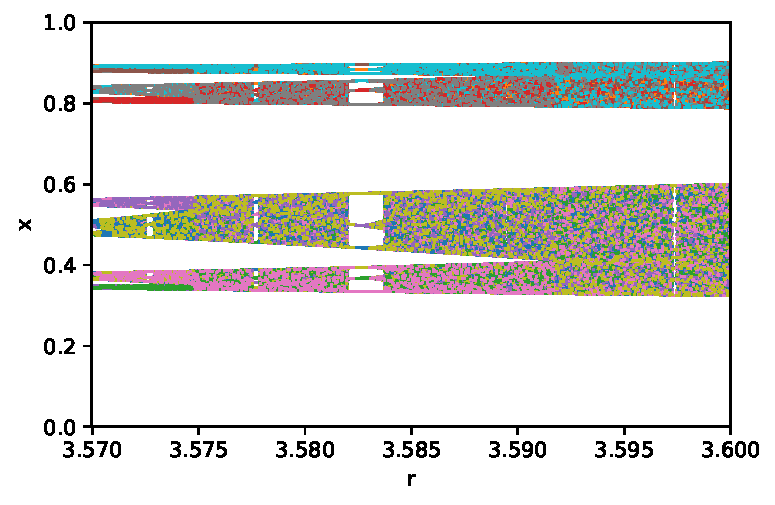
\includegraphics[keepaspectratio]{01-logistica/Caos_files/figure-pdf/cell-2-output-1.pdf}}
  \caption{Partición en dos bandas de la zona caótica (i)}
\end{figure}    

A medida que subimos \(r\), esas dos bandas se bifurcan en 4, luego en
8, repitiendo la misma lógica de duplicación pero sobre la estructura
del caos.

\begin{figure}[h]
  \centering
  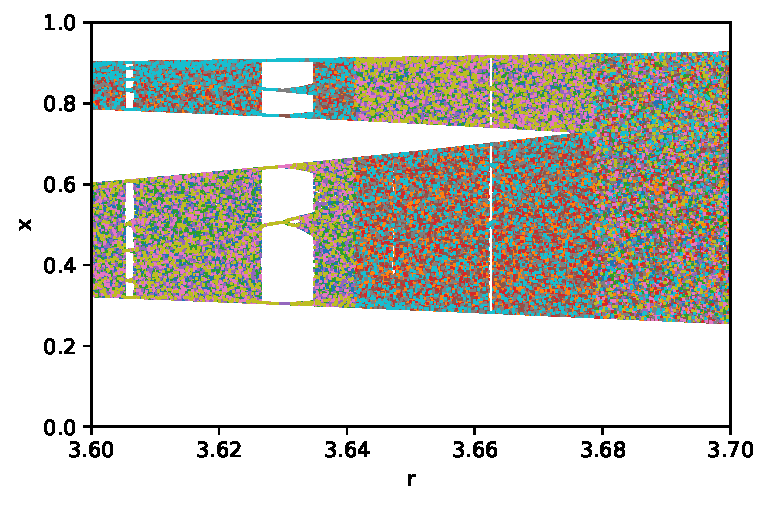
\includegraphics[keepaspectratio]{01-logistica/Caos_files/figure-pdf/cell-3-output-1.pdf}}
  \caption{Partición en dos bandas de la zona caótica (ii)}
\end{figure}


\section{Ventanas de periodicidad}\label{ventanas-de-periodicidad}

En medio del caos surgen \textbf{islas} de orden donde aparece un ciclo
estable de periodo \(k\) (por ejemplo, un ciclo de orden 3 alrededor de
\(r\approx3.828\)).

\begin{figure}[h]
  \centering
  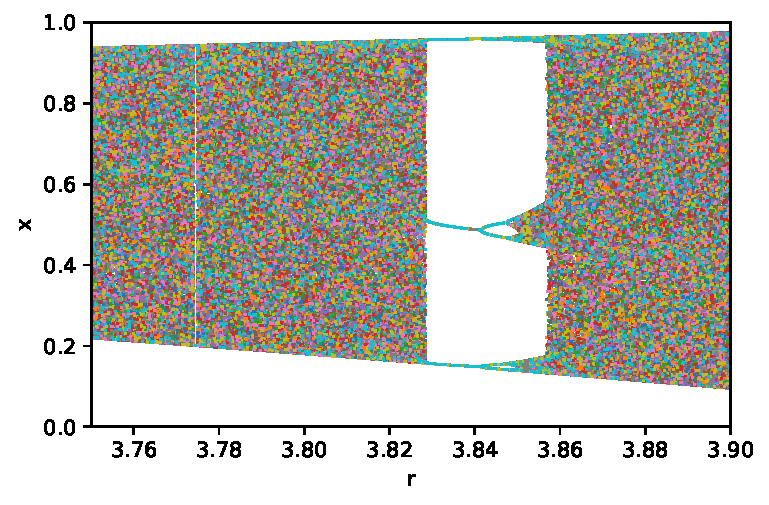
\includegraphics[keepaspectratio]{01-logistica/Caos_files/figure-pdf/cell-4-output-1.pdf}}
  \caption{Islas periódicas en la zona caótica}
\end{figure}


Dentro de cada ventana periódica se reproduce una \textbf{mini-cascada}
de duplicación de periodo \(k \to 2k \to 4k \to \cdots\). Lo mismo que
teníamos en la zona \(3 < r < 3.56995\) pero ahora dentro de la zona
caótica. Vemos como el caos da paso de nuevo a las órbitas periódicas

\begin{figure}[h]
  \centering
  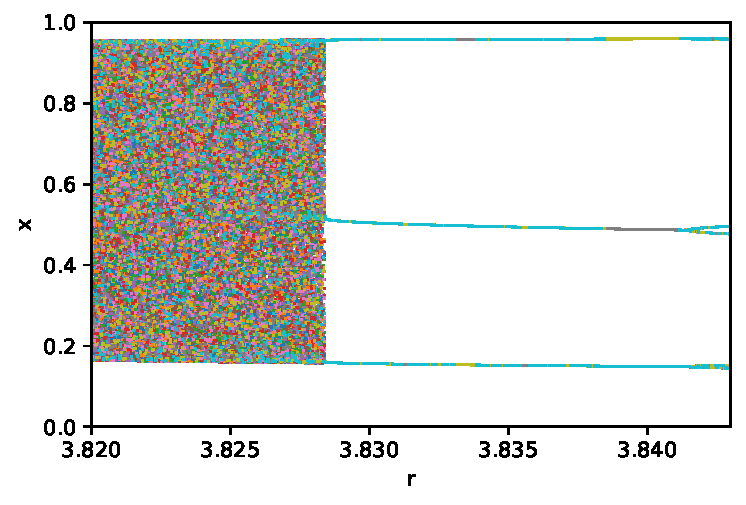
\includegraphics[keepaspectratio]{01-logistica/Caos_files/figure-pdf/cell-5-output-1.pdf}}
  \caption{Islas periódicas en la zona caótica (zoom)}
\end{figure}

\section{Repetición infinita}\label{repeticiuxf3n-infinita}

Las ventanas de periodicidad están \textbf{infinitamente repetidas}: en
cada fragmento de la región caótica, por pequeño que sea, habrá alguna
ventana donde emerja un ciclo estable.

Así vemos como entre 3.73 y 3.76 aparecen un ciclo de período 5.

\pandocbounded{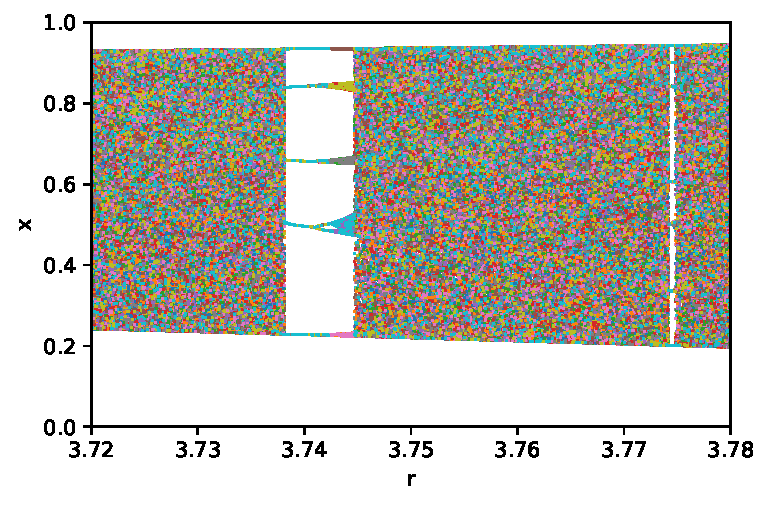
\includegraphics[keepaspectratio]{01-logistica/Caos_files/figure-pdf/cell-6-output-1.pdf}}

\begin{figure}[h]
  \centering
  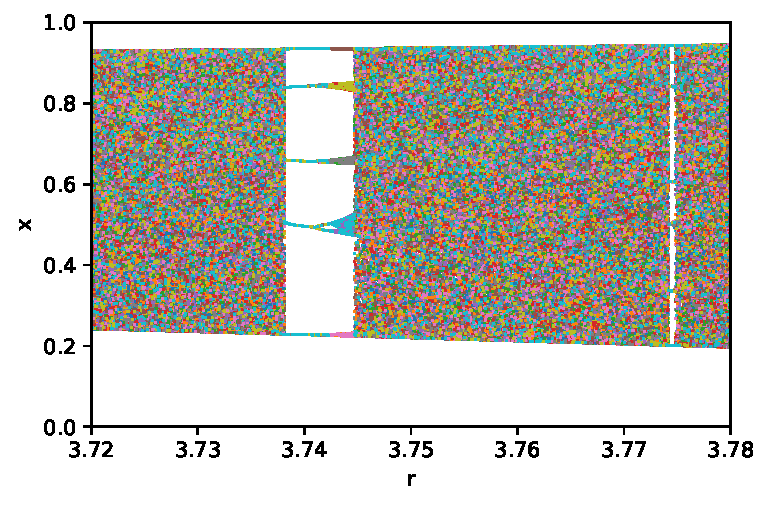
\includegraphics[keepaspectratio]{01-logistica/Caos_files/figure-pdf/cell-6-output-1.pdf}}
  \caption{Ciclo de período 5 entre 3.73 y 3.76}
\end{figure}


Si nos centramos en los valores de x alrededor de 0.5, vemos claramente
el diagrama de bifurcación inicial replicado aquí, con tan solo 1000
iteraciones.

\begin{figure}[h]
  \centering
  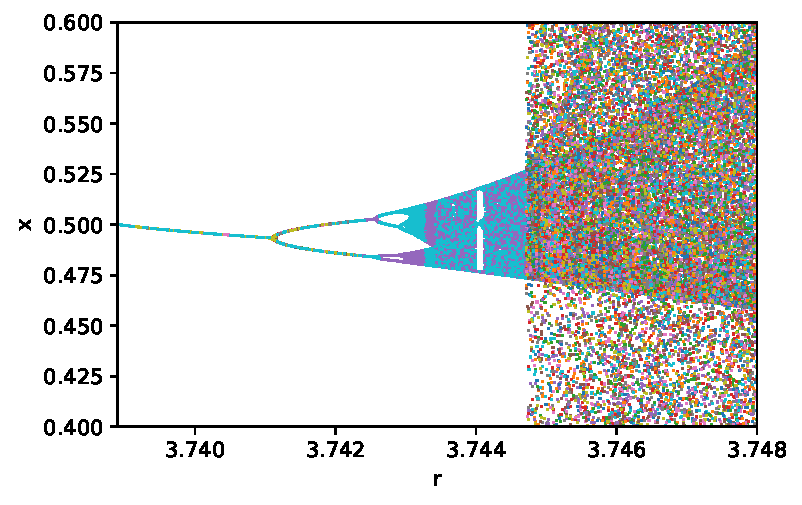
\includegraphics[keepaspectratio]{01-logistica/Caos_files/figure-pdf/cell-7-output-1.pdf}}
  \caption{Réplica del diagrama de bifurcación original}
\end{figure}


Y dentro de esta replicación del diagrama de bifurcación original,
podemos encontrar el ciclo de periodo 5 de nuevo, en los valores de
\(r\) comprendidos entre 3.74431 y 3.74433.

\begin{figure}[h]
  \centering
  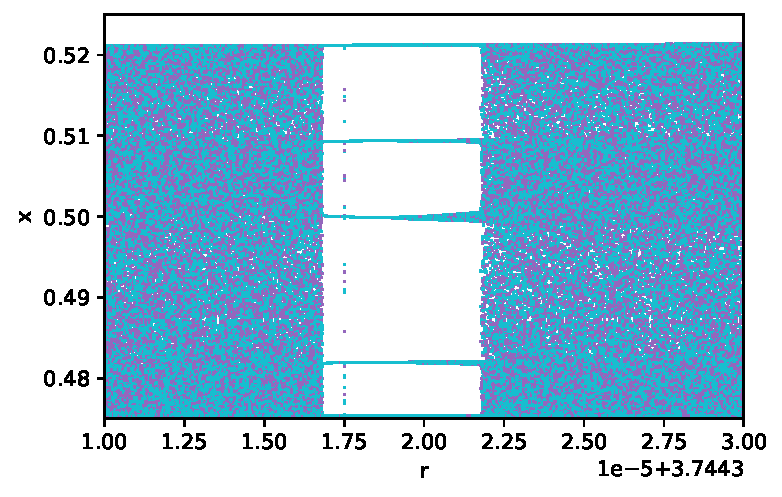
\includegraphics[keepaspectratio]{01-logistica/Caos_files/figure-pdf/cell-8-output-1.pdf}}
  \caption{Réplica del ciclo de período 5 entre 3.74431 y 3.74433}
\end{figure}

Y de nuevo, cogemos la replicación del diagrama de bifurcación original
alrededor de 0.5 y nos encontramos con el ciclo de periodo 5 de nuevo,
en los valores de \(r\) comprendidos entre 3.74432144 y 3.744321455.
Cada vez necesitaremos más iteraciones para apreciar el diagrama de
bifurcación original. De hecho, para plotear esta última gráfica se han
requerido 100.000 iteraciones


\begin{figure}[h]
  \centering
  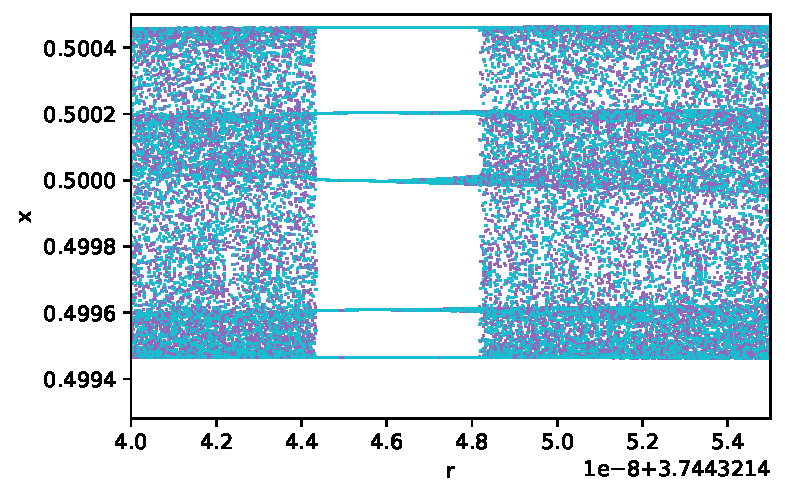
\includegraphics[keepaspectratio]{01-logistica/Caos_files/figure-pdf/cell-9-output-1.pdf}}
  \caption{Réplica del ciclo de período 5 entre 3.74432144 y 3.744321455}
\end{figure}


Haciendo de nuevo zoom en torno a 0.5, vemos como aparece el diagrama de
bifurcación original, esta vez en los valores de \(r\) comprendidos
entre 3.7443214444 y 3.744321448 , tras 1.000.000 de iteraciones.


\begin{figure}[h]
  \centering
  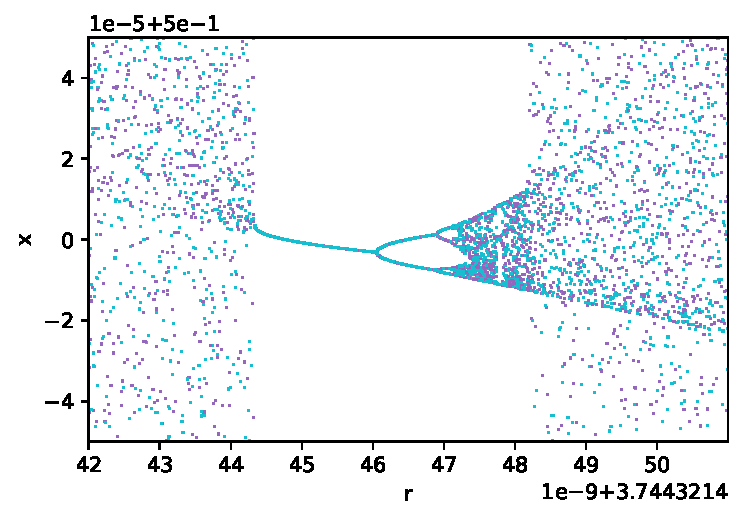
\includegraphics[keepaspectratio]{01-logistica/Caos_files/figure-pdf/cell-10-output-1.pdf}}
  \caption{Réplica del diagrama de bifurcación original entre 3.7443214444 y 3.744321448 }
\end{figure}

Podemos seguir así infinitamente. Lo que hemos encontrado es una
\textbf{estructura fractal}.

\chapter{Efecto mariposa}\label{efecto-mariposa}

\section{Sensibilidad a las condiciones
iniciales}\label{sec-sensibilidad}

Cuando estamos en la zona estable del mapa logístico, desde cualquier
valor de \(x_0\) del que partamos, llegaremos siempre hasta el mismo
valor final, bien sea el punto fijo que hemos calculado previamente, o
cualquiera de los valores de las órbitas periódicas. Por ejemplo, para
\(r=2.8\)

\begin{figure}[h]
  \centering
  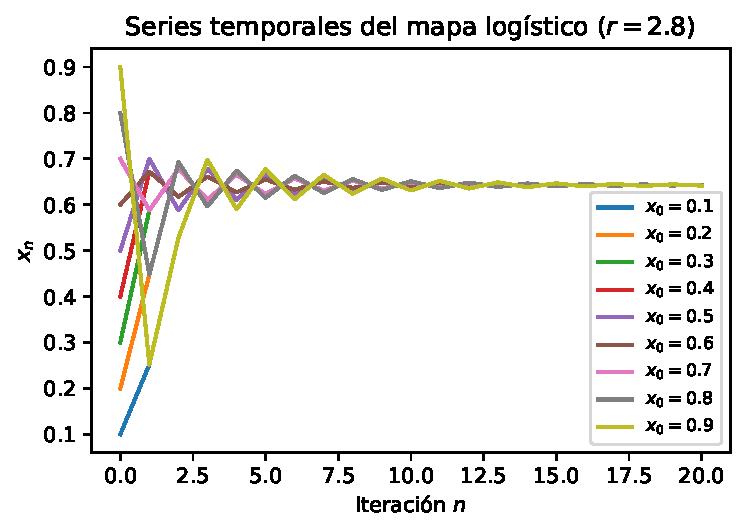
\includegraphics[keepaspectratio]{01-logistica/lyapunov_files/figure-pdf/cell-2-output-1.pdf}
  \caption{Valor final del mapa logístico en zona no caótica}
\end{figure} 

Y para \(r=3.1\), vemos como también los puntos alcanzados son los
mismos para valores próximos de inicio de la sucesión.

\begin{figure}[h]
  \centering
  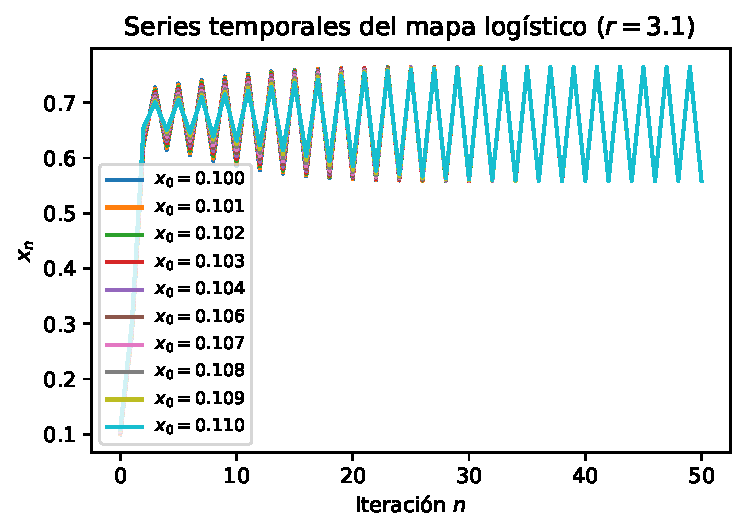
\includegraphics[keepaspectratio]{01-logistica/lyapunov_files/figure-pdf/cell-3-output-1.pdf}
  \caption{Valor final del mapa logístico en zona de primera bifurcación}
\end{figure} 

En los dos casos anteriores, no parece que la evolución del sistema sea
sensible a la condición inicial de partida. Tras unas pocas iteraciones,
da igual de donde se parta, que se converge al mismo punto.

Pero, ¿qué pasa cuando estamos en las zonas caóticas?. Veamos la
iteración del mapa logístico para \(r=3.69\) partiendo de dos valores
muy similares, que solo se separan en \(10^{-5}\) unidades.

\begin{figure}[h]
  \centering
  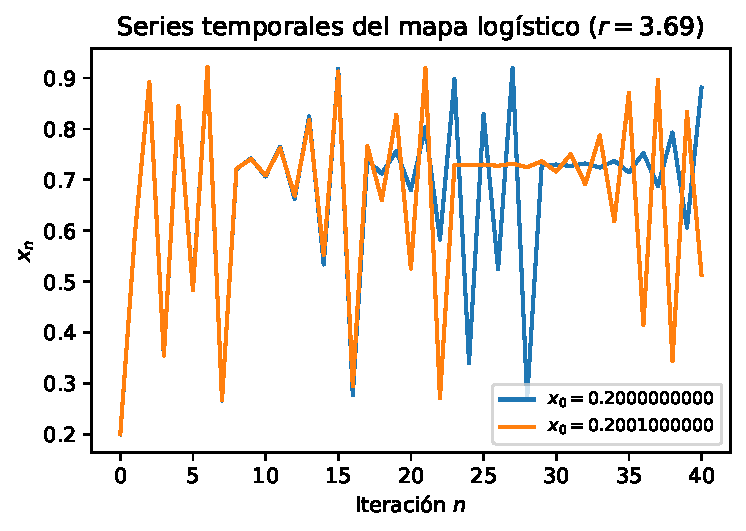
\includegraphics[keepaspectratio]{01-logistica/lyapunov_files/figure-pdf/cell-4-output-1.pdf}
  \caption{Valor final del mapa logístico en zona de caótica con dos condiciones iniciales ligeramente distintas}
\end{figure} 

A la vista del gráfico, vemos como a partir de la iteración 10 empiezan
a haber pequeñas diferencias que se van amplificando a medida que avanza
la simulación. Aquí vemos que sí que empieza a haber sensibilidad a las
condiciones iniciales.

Probemos con una diferencia de valores iniciales aún mas pequeña, en
este caso \(10^{-7}\) unidades.

\begin{figure}[h]
  \centering
  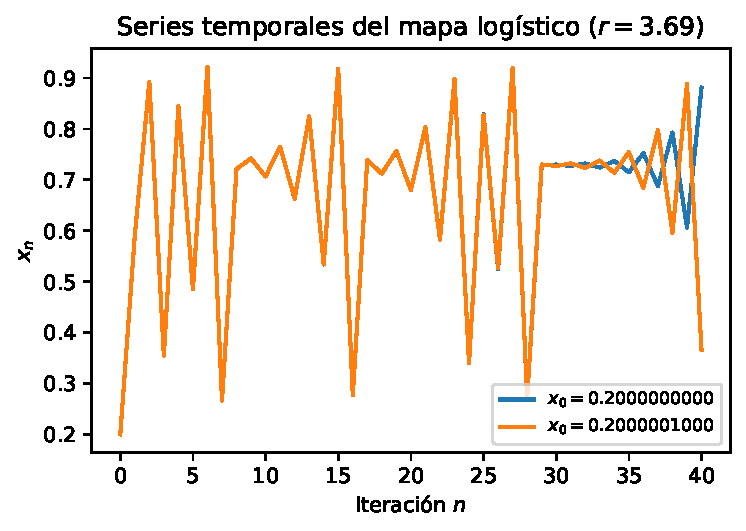
\includegraphics[keepaspectratio]{01-logistica/lyapunov_files/figure-pdf/cell-5-output-1.pdf}
  \caption{Valor final del mapa logístico en zona de caótica con dos condiciones iniciales ligeramente distintas}
\end{figure}    

Ahora la separación de ambas simulaciones se produce a partir de la
iteración número 30. Vamos con una diferencia aún mas pequeña, ahora
\(10^{-10}\) unidades.

\begin{figure}[h]
  \centering
  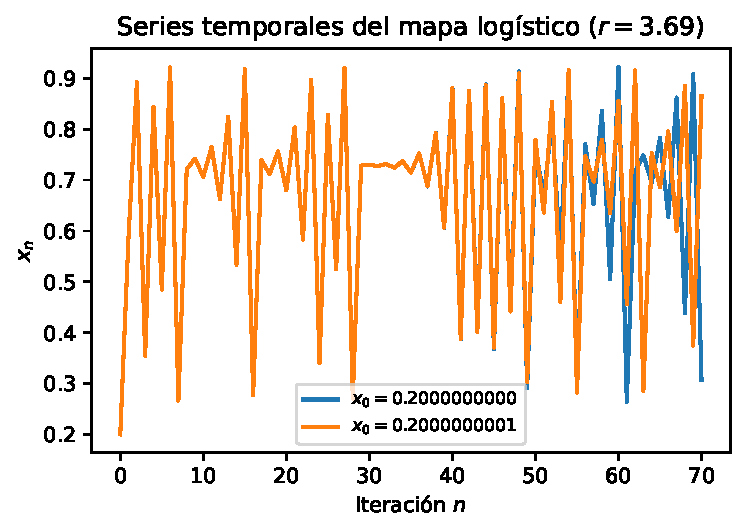
\includegraphics[keepaspectratio]{01-logistica/lyapunov_files/figure-pdf/cell-6-output-1.pdf}
  \caption{Valor final del mapa logístico en zona de caótica con dos condiciones iniciales ligeramente distintas}
\end{figure}  


La separación entre ambas curvas empieza a hacerse visible a partir de
la iteración 50. ¿Qué pasa si hacemos la diferencia aún más pequeña, en
este caso \(10^{-15}\) unidades?. Pues como vemos en la siguiente
gráfica, a partir de la iteración 85 empezamos a ver la divergencia de
ambas sucesiones.

\begin{figure}[h]
  \centering
  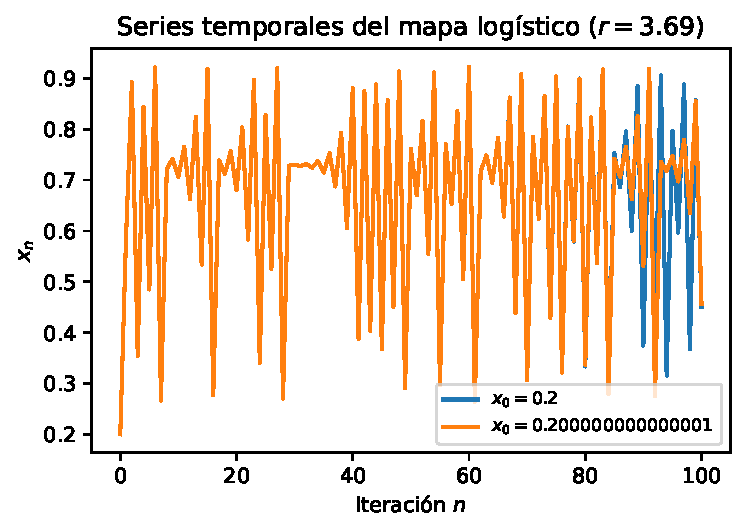
\includegraphics[keepaspectratio]{01-logistica/lyapunov_files/figure-pdf/cell-7-output-1.pdf}
  \caption{Valor final del mapa logístico en zona de caótica con dos condiciones iniciales ligeramente distintas}
\end{figure}  


¿Qué está pasando aquí?. ¿Cómo puede ser que dos valores iniciales que
se diferencian en un valor tan pequeño como \(10^{-15}\) unidades den
valores tan diferentes tras 100 iteraciones?. Si las unidades fueran
metros, estaríamos hablando de una diferencia de un femtómetro. Y aún
más importante: si quiero simular un sistema físico como éste en la
región caótica, ¿cómo voy a poder medir su condición inicial con tal
precisión?. De hecho, parece que la precisión requerida sería infinita.
A poco que me equivoque en la estimación de la condición inicial, no voy
a poder calcular bien su estado final pasado un número grande de
iteraciones. ¿Cómo puede ser si mi sistema es determinista y está regido
por una ecuación tan sencilla?. Hemos topado con el caos y el
\textbf{efecto mariposa}. Y lo inquietante es que este fenómeno se da en
sistemas físicos como la meteorología.

\subsection{Inestabilidad de los cálculos
numéricos}\label{sec-inestabilidad}

Cuando nos encontramos con un sistema físico con alta dependencia a las
condiciones iniciales, no solamente tenemos el problema de conocer con
total exactitud el estado inicial del sistema, sino que como veremos a
continuación, los cálculos numéricos que hacemos en nuestro ordenador
para estudiar su evolución se vuelven también muy inestables. A
continuación pondré un ejemplo sobre lo que acabo de decir.

Pongamos que quiero simular el mapa logístico tal cual lo he estado
haciendo en las secciones anteriores. La fórmula es superconocida
(form1):

\begin{equation}
x_{n+1} = r\,x_n\,(1 - x_n)
\end{equation}

Pero también podríamos expresarlo como (form2):

\begin{equation}
x_{n+1} = r\,x_n - r\,{x_n}^2
\end{equation}

Matemáticamente son equivalentes pero a un computador le estamos
diciendo cosas diferentes. * En el primer caso le decimos que reste 1
menos \{x\_n\}, y que a continuación lo multiplique por \(r\) y \(x_n\).
En total 1 resta y dos multiplicaciones * En el segundo caso le decimos
que multiplique por \(r\) y \(x_n\) por un lado. Por otro lado que que
eleve \(x_n\) al cuadrado, y que lo multiplique por \(r\). Y al final
que reste el primer resultado intermedio menos el segundo. En total 1
resta, 2 multiplicaciones y 1 cuadrado.

A esto hay que añadir que en un ordenador los números decimales se
representan mediante aproximaciones. Por ejemplo, con 32 bits,el número
0.2 se representa como 0.200000003, debido a la precisión finita que dan
los 32 bits. Por lo tanto entre el número real y el que representamos,
la mayoría de veces va a haber un error. Estos errores se comportarán de
manera diferente según los cálculos aritméticos que hagamos con ellos.
En el siguiente plot, vemos los errores en un ordenador entre las dos
fórmulas al partir del valor \(x_0=0.2\) y con un \(r=4\).

\begin{figure}[h]
  \centering
  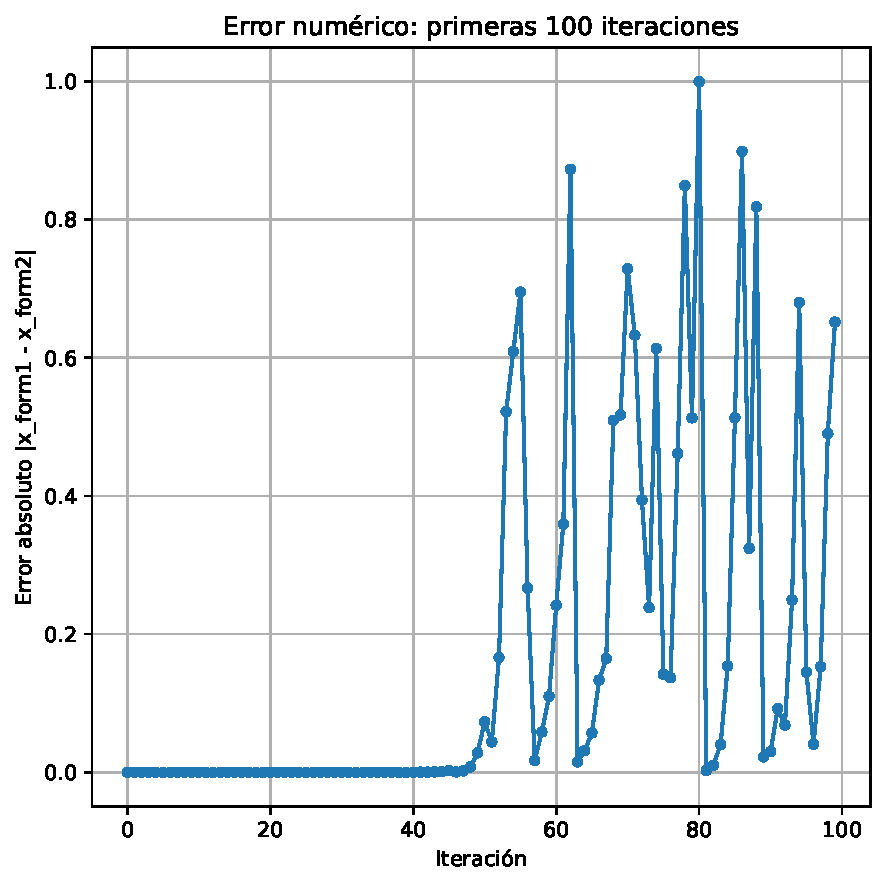
\includegraphics[keepaspectratio]{01-logistica/lyapunov_files/figure-pdf/cell-8-output-1.pdf}
  \caption{Error numérico entre las dos fórmulas matemáticamente equivalentes tras 100 iteraciones}
\end{figure}  



Vemos como al principio el error es imperceptible, pero a media que
avanzamos va creciendo. A partir de la iteración 50 este error se hace
ya notable, y desde entonces se puede decir que ambas fórmulas
evolucionan de forma totalmente distinta. Por lo tanto, vemos como en un
sistema caótico, no sólo las condiciones iniciales determinan el valor
final de forma extrema, sino que también cuando simulamos este sistema
en una máquina computacional, la forma en la que se representan los
números y la forma de las operaciones también influyen de forma muy
notable. Esto es otra manifestación del caos, y se le denomina \textbf{efecto polilla} . 

Pero vamos a ir un paso más. Veamos que evolución tienen realmente los
errores. Para poder bien los errores al principio y al final, vamos a
usar una escala logarítmica en el eje Y. El resultado se muestra a
continuación.

\begin{figure}[h]
  \centering
  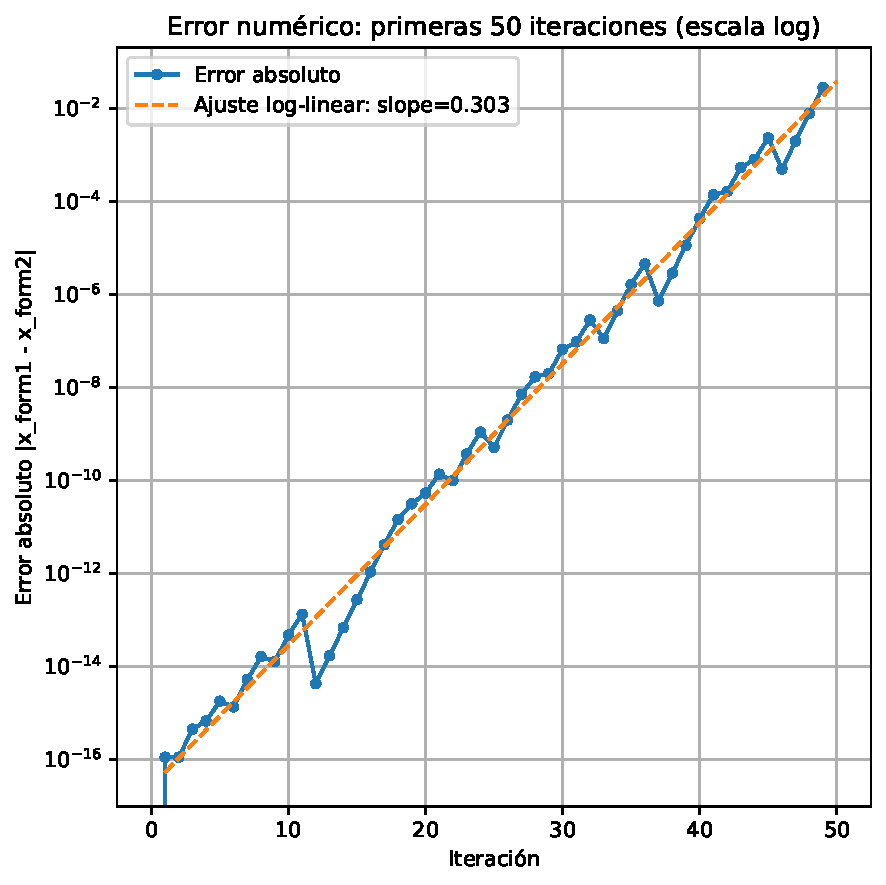
\includegraphics[keepaspectratio]{01-logistica/lyapunov_files/figure-pdf/cell-9-output-1.pdf}
  \caption{Error numérico entre las dos fórmulas matemáticamente equivalentes tras 100 iteraciones (escala logarítmica)}
\end{figure}  


¿Qué es lo que vemos?. Que los errores crecen linealmente dentro de la
escala logarítmica.

En escala \(\log_{10}\) hemos ajustado: \[
\log_{10}(\mathrm{error}_n)\approx 0.303\,n + C
\] donde \(C\) es la ordenada en el origen. Pasando de logaritmos a
forma explícita: \[
\mathrm{error}_n \approx 10^C \times 10^{0.303\,n}
= A\,\bigl(10^{0.303}\bigr)^n
\approx A\,2^n,
\] puesto que \(10^{0.303}\approx2\).

Equivalentemente, en base \(e\): \[
\ln(\mathrm{error}_n)
= \ln(10)\,\log_{10}(\mathrm{error}_n)
\approx (0.303\,\ln 10)\,n + \ln A
\approx 0.698\,n + \ln A,
\] de donde \[
\mathrm{error}_n \approx A\,e^{0.698\,n}\approx A\,(2.01)^n.
\]

\textbf{Conclusión.} El error crece de forma \textbf{exponencial} con
\(n\), aproximadamente duplicándose en cada iteración.

Curioso, ¿verdad?. El error se va multiplicando por 2 en cada iteración.
Por 2 exactamente. ¿A qué se debe esto????

\section{Cálculo matemático de la amplificación de desviaciones
iniciales}\label{cuxe1lculo-matemuxe1tico-de-la-amplificaciuxf3n-de-desviaciones-iniciales}

A continuación daremos una explicación matemática a este fenómeno que
estamos observando.

Imagina que quieres predecir el tiempo atmosférico. Nunca conoces la
temperatura, presión o humedad con absoluta precisión: siempre hay un
error mínimo en la medición. Si ese error crece muy despacio, podrías
predecir con confianza varios días por delante. Pero si crece muy
rápido, tu predicción se vuelve inútil en muy poco tiempo.

En los siguientes párrafos, veremos un concepto matemático muy útil en el
estudio del caos: el \textbf{exponente de Lyapunov}, que llamaremos
\(\lambda\) y que cuantifica la tasa de crecimiento de estos errores. Este concepto será fundamental en el estudio de sistemas físicos como el péndulo doble y la atmósfera. Nos permitirá saber de forma fácil el grado de "caoticidad" de un sistema. 

\subsection{Error inicial}\label{error-inicial}

\begin{itemize}
\tightlist
\item
  Sea \(x_0\) el estado ``verdadero'' del sistema en el tiempo
  inicial.\\
\item
  Tu medida real tiene un pequeño error \(\delta_0\), de modo que en
  realidad partes de\\
  \[
     x_0 + \delta_0,
     \quad\text{con}\;|\delta_0|\ll 1.
   \]
\end{itemize}

Ese \(\delta_0\) es tan pequeño que, al principio, los dos estados están
casi juntos. Es lo que hemos visto en los ejemplos anteriores, donde en
la primera iteración las dos simulaciones estaban casi juntas.

\subsection{Cómo evoluciona el error}\label{cuxf3mo-evoluciona-el-error}

Supón que el sistema avanza según una regla \(f\) (nuestra función
logística), es decir: \[
x_{n+1} = f(x_n).
\] Queremos ver qué sucede con \(\delta_n\), la diferencia en el paso
\(n\). Para ello:

\begin{enumerate}
\def\labelenumi{\arabic{enumi}.}
\item
  \textbf{Linealizamos} la función \(f\) alrededor de \(x_n\).\\
  Si \(f\) es suave, podemos aproximar \[
    f(x_n + \delta_n)
    \approx f(x_n)
         + f'(x_n)\,\delta_n,
  \] donde \(f'(x_n)\) es la \textbf{derivada} (o pendiente) de \(f\) en
  \(x_n\).
\item
  De esta aproximación se deduce que \[
    \delta_{n+1} 
    = f(x_n + \delta_n) - f(x_n)
    \approx f'(x_n)\,\delta_n.
  \]
\end{enumerate}

Pero ojo. Cuando calculamos errores, siempre son distancia, es decir
debe ser siempre un número no negativo. La derivada indica pendiente y
sentido.Cuando linealizamos\\
\[
   f(x_n + \delta_n)\approx f(x_n) + f'(x_n)\,\delta_n,
   \]\\
el término \(f'(x_n)\,\delta_n\) nos da \textbf{cuánto} y en \textbf{qué
dirección} cambia la diferencia \(\delta_n\).

La distancia ha de ser siempre no negativa. Por tanto, definimos : \[
   \delta_{n+1} = \bigl|\,x'_{n+1} - x_{n+1}\bigr|.
   \]\\
Sin valor absoluto, un \(f'(x_n)<0\) haría que la ``distancia''
resultase negativa, lo cual no tiene sentido para una medida de error.

El verdadero error en módulo es \(\bigl|f'(x_n)\bigr|\)\$ porque:

\begin{itemize}
\tightlist
\item
  Si \(\lvert f'(x_n)\rvert>1\), la distancia \textbf{aumenta}\\
\item
  Si \(\lvert f'(x_n)\rvert<1\), la distancia \textbf{disminuye}
\end{itemize}

Pongamos un ejemplo numérico: Supongamos \(f'(x_n)=-2\) y
\(\delta_n=0.01\):

\begin{itemize}
\tightlist
\item
  Sin valor absoluto:\\
  \[
  \delta_{n+1}\approx(-2)\times0.01=-0.02\quad(\text{sin sentido físico}).
  \]\\
\item
  Con valor absoluto:\\
  \[
  \delta_{n+1}\approx\bigl|-2\bigr|\times0.01=2\times0.01=0.02,
  \]\\
  reflejando correctamente que la distancia se \textbf{duplica}.
\end{itemize}

Por todo ello, la fórmula adecuada para la evolución del error es\\
\[
\delta_{n+1} \approx \bigl|f'(x_n)\bigr|\,\delta_n,
\]\\
garantizando que \(\delta_{n+1}\ge0\) y midiendo la \textbf{magnitud}
real del estiramiento en cada paso.

\section{Errores sucesivos}\label{errores-sucesivos}

Si repetimos la relaciones anterior paso a paso obtenemos

\begin{enumerate}
\def\labelenumi{\arabic{enumi}.}
\item
  Primera iteración\\
  \[
  \delta_1 \approx \bigl|f'(x_0)\bigr|\,\delta_0.
  \]
\item
  Segunda iteración. En este caso es la derivada en \(x_1\) multiplicado
  por el error anterior (utilizamos para el error anterior la fórmula
  del paso 1). En total vemos que el error en la segunda iteración, es
  el error inicial multiplicado por dos derivadas. \[
  \delta_2
  \approx \bigl|f'(x_1)\bigr|\,\delta_1
  \approx \bigl|f'(x_1)\bigr|\;\bigl|f'(x_0)\bigr|\;\delta_0.
  \]
\item
  Tercera iteración. Aquí ya vemos como aparece un patrón. Vamos
  multiplicando el error inicial por las sucesivas derivadas. \[
  \delta_3
  \approx \bigl|f'(x_2)\bigr|\,\delta_2
  \approx \bigl|f'(x_2)\bigr|\;\bigl|f'(x_1)\bigr|\;\bigl|f'(x_0)\bigr|\;\delta_0.
  \]
\end{enumerate}

En general, para cualquier (n\ge1) podemos generalizar el patrón
encontrado:\\
\[
\delta_n
\;\approx\;
\Bigl(\prod_{k=0}^{n-1}\bigl|f'(x_k)\bigr|\Bigr)\;\delta_0.
\]


Este resultado es muy parecido al de la estabilidad de los puntos fijos. Animo al lector a visitar \url{https://colacaos.github.io/ColaCAOS/01-logistica/puntos-fijos.html#estudio-formal-de-la-convergencia} para ver como también en ese caso la estabilidad venía dada por el valor de la primera derivada. 

\section{De producto a suma}\label{de-producto-a-suma}

Para manejar productos es muy útil usar los logaritmos, porque
transforman productos en sumas: \[
\ln\bigl(\delta_n/\delta_0\bigr)
= \ln\Bigl(\prod_{k=0}^{n-1} f'(x_k)\Bigr)
= \sum_{k=0}^{n-1}\ln\bigl|f'(x_k)\bigr|.
\]

Esta formula nos da el logaritmo de cuánto ha crecido el error tras n
iteraciones en relación al error inicial.

\section{\texorpdfstring{Definición del exponente de Lyapunov
\(\lambda\)}{Definición del exponente de Lyapunov \textbackslash lambda}}\label{definiciuxf3n-del-exponente-de-lyapunov-lambda}

Sabemos según la fórmula anterior, cuánto ha crecido el error en \(n\)
iteraciones. Ahora bien, estaría mejor saber cuanto crece de media por
cada iteración. Para ello, solo tenemos que dividir la suma anterior
entre \(n\).

\begin{equation}
\frac{1}{n}\,\sum_{k=0}^{n-1}\ln\bigl|f'(x_k)\bigr|.
\end{equation}

Ahora vamos a suponer que la simulación es muy larga y que queremos
hacer un promedio. Para ello tomamos el límite cuando \(n\to\infty\) de
la expresión anterior: \[
\lambda
= \lim_{n\to\infty}
\frac{1}{n}\,\sum_{k=0}^{n-1}\ln\bigl|f'(x_k)\bigr|.
\]

Este factor \(\lambda\) es lo que crece de media el error en cada
iteración en mi sistema. LO que crece de forma logarítmica. Lo que crece
realmente en magnitud en cada iteración es \(e^\lambda\)

\begin{itemize}
\tightlist
\item
  Si \(\lambda>0\), el error crece con cada iteración, puesto que el
  número \(e\) elevado a un valor positivo siempre da un número mayor
  que 1. Puesto que multiplico mi error por un número mayor que 1, el
  error va creciendo iteración tras iteración
  (\(e^\lambda\)\(e^\lambda\)\(e^\lambda\)\ldots\ldots=\((e^\lambda)^n\)=\(a^n\)
  con \(a>1\)) . Crece por lo tanto \textbf{exponencialmente}, y el
  sistema es \textbf{caótico} (muy sensible a la precisión inicial).
\item
  Si \(\lambda<0\), el error \textbf{se atenúa} y las trayectorias
  convergen (sistema estable).La argumentación es justa la contraria del
  caso anterior. El número \(e\) elevado a un valor negativo siempre da
  un número menor que 1.
\item
  Si \(\lambda=0\), estamos en un caso límite de inestabilidad neutra.
\end{itemize}

\section{Cálculo del exponente de Lyapunov para el mapa
logístico}\label{cuxe1lculo-del-exponente-de-lyapunov-para-el-mapa-loguxedstico}

Consideramos el \textbf{mapa logístico}\\
\[
x_{n+1} = f(x_n) = r\,x_n\,(1 - x_n),
\]

La derivada de \(f\), tal y como hemos visto en anteriores secciones,
es\\
\[
f'(x) = r\,(1 - 2x).
\]

Por lo tanto, si tenemos una sucesión de puntos compuesta por
\(x_0, x_1, \dots, x_{N}\), el exponente de Lyapunov máximo se calculará
a partir de la multiplicación de las derivadas de la función logística
en cada uno de los puntos de la sucesión, es decir,

\begin{equation}
\lambda = \lim_{N\to\infty} \frac{1}{N} \sum_{n=0}^{N-1} \ln\bigl|f'(x_n)\bigr|
        = \lim_{N\to\infty} \frac{1}{N} \sum_{n=0}^{N-1} \ln\bigl|r\,(1 - 2x_n)\bigr|.
\end{equation}

En la práctica, no podemos llevar la sucesión al infinito, por lo que
tomamos N iteraciones y aplicamos la siguiente fórmula aproximada

\[
\lambda_N = \frac{1}{N} \sum_{k=0}^{N-1} \ln\bigl|f'(x_k)\bigr|
= \frac{1}{N} \sum_{k=0}^{N-1} \ln\bigl|4\,(1 - 2x_k)\bigr|.
\]\\
Al aumentar \(N\), \(\lambda_N\) tenderá a \(\lambda\).

\subsection{\texorpdfstring{Ejemplo numérico sencillo
(\(N=20\))}{Ejemplo numérico sencillo (N=20)}}\label{sec-exponente}

Vamos a calcular el exponente de Lyapunov para el caso de \(r=4\). Tal y
como vimos en las simulaciones que hicimos en el primer apartado, con
\(r=4\) se prevé que el error se vaya doblando en cada paso, o lo que es
lo mismo, que el exponente de Lyapunov sea
\(\lambda = \ln 2 \approx 0.6931\)

Tomemos de nuevo el mapa logístico con \(r = 4\), es decir, \[
f(x) = 4x(1 - x),
\] y su derivada \[
f'(x) = 4(1 - 2x).
\] Queremos calcular el exponente de Lyapunov aproximado usando \(20\)
iteraciones, empezando con \[
x_{0} = 0.3000
\] Para ello, iremos calculando sucesivamente cada
\(x_{n+1} = f(x_{n})\), el valor absoluto de la derivada
\(\lvert f'(x_{n})\rvert\), y luego \(\ln\lvert f'(x_{n})\rvert\).
Mostraremos en la siguiente tabla \(x_{n}\) redondeado a cuatro cifras
decimales, \(\lvert f'(x_{n})\rvert\) redondeado a cuatro cifras
decimales, y \(\ln\lvert f'(x_{n})\rvert\) redondeado a tres cifras
decimales.

\begin{longtable}[]{@{}
  >{\centering\arraybackslash}p{(\linewidth - 6\tabcolsep) * \real{0.0806}}
  >{\centering\arraybackslash}p{(\linewidth - 6\tabcolsep) * \real{0.1613}}
  >{\centering\arraybackslash}p{(\linewidth - 6\tabcolsep) * \real{0.4677}}
  >{\centering\arraybackslash}p{(\linewidth - 6\tabcolsep) * \real{0.2903}}@{}}
\caption{Cálculo paso a paso del exponente de Lyapunov para \(r=4\)}\label{tab:lyapunov}\\
\toprule\noalign{}
\begin{minipage}[b]{\linewidth}\centering
\(n\)
\end{minipage} & \begin{minipage}[b]{\linewidth}\centering
\(x_{n}\)
\end{minipage} & \begin{minipage}[b]{\linewidth}\centering
\(|f'(x_{n})|\)
\end{minipage} & \begin{minipage}[b]{\linewidth}\centering
\(\ln|f'(x_{n})|\)
\end{minipage} \\
\midrule\noalign{}
\endhead
\bottomrule\noalign{}
\endlastfoot
0 & 0.3000 & \(|4(1 - 2\cdot0.3000)| = 1.6000\) & 0.470 \\
1 & 0.8400 & \(|4(1 - 2\cdot0.8400)| = 2.7200\) & 1.001 \\
2 & 0.5376 & \(|4(1 - 2\cdot0.5376)| = 0.3008\) & -1.201 \\
3 & 0.9953 & \(|4(1 - 2\cdot0.9953)| = 3.9548\) & 1.375 \\
4 & 0.0186 & \(|4(1 - 2\cdot0.0186)| = 3.8201\) & 1.340 \\
5 & 0.0879 & \(|4(1 - 2\cdot0.0879)| = 3.2964\) & 1.193 \\
6 & 0.3208 & \(|4(1 - 2\cdot0.3208)| = 1.4332\) & 0.360 \\
7 & 0.8716 & \(|4(1 - 2\cdot0.8716)| = 2.9729\) & 1.090 \\
8 & 0.4476 & \(|4(1 - 2\cdot0.4476)| = 0.4191\) & -0.870 \\
9 & 0.9890 & \(|4(1 - 2\cdot0.9890)| = 3.9122\) & 1.364 \\
10 & 0.0434 & \(|4(1 - 2\cdot0.0434)| = 3.6526\) & 1.295 \\
11 & 0.1661 & \(|4(1 - 2\cdot0.1661)| = 2.6708\) & 0.982 \\
12 & 0.5542 & \(|4(1 - 2\cdot0.5542)| = 0.4333\) & -0.836 \\
13 & 0.9883 & \(|4(1 - 2\cdot0.9883)| = 3.9061\) & 1.363 \\
14 & 0.0464 & \(|4(1 - 2\cdot0.0464)| = 3.6289\) & 1.289 \\
15 & 0.1770 & \(|4(1 - 2\cdot0.1770)| = 2.5844\) & 0.949 \\
16 & 0.5826 & \(|4(1 - 2\cdot0.5826)| = 0.6605\) & -0.415 \\
17 & 0.9727 & \(|4(1 - 2\cdot0.9727)| = 3.7819\) & 1.330 \\
18 & 0.1061 & \(|4(1 - 2\cdot0.1061)| = 3.1512\) & 1.148 \\
19 & 0.3794 & \(|4(1 - 2\cdot0.3794)| = 0.9651\) & -0.036 \\
\end{longtable}

Cada fila se interpreta así:

\begin{enumerate}
\def\labelenumi{\arabic{enumi}.}
\tightlist
\item
  Calculamos \(x_{n+1} = 4\,x_{n}\,(1 - x_{n})\) usando el valor exacto
  de \(x_{n}\) y luego redondeamos el resultado a cuatro decimales para
  mostrarlo.
\item
  Evaluamos la derivada en el valor exacto de \(x_{n}\):
  \(f'(x_{n}) = 4(1 - 2x_{n})\), tomamos su valor absoluto, y lo
  redondeamos a cuatro decimales.
\item
  Finalmente, calculamos \(\ln\lvert f'(x_{n})\rvert\) a partir del
  valor de la derivada ya redondeada, y lo redondeamos a tres decimales.
\end{enumerate}

Ahora sumamos todos los logaritmos obtenidos: \[
\begin{align}
\sum_{k=0}^{19} \ln\lvert f'(x_{k})\rvert \;=\;& 
0.470 + 1.001 \;-\; 1.201 + 1.375 + 1.340 + 1.193 + 0.360 + 1.090 \;-\; 0.870 + 1.364 \\
&+ 1.295 + 0.982 \;-\; 0.836 + 1.363 + 1.289 + 0.949 \;-\; 0.415 + 1.330 + 1.148 \;-\; 0.036 \\
=\;& 13.191.
\end{align}
\] Por último promediamos esta suma, por lo que el exponente de Lyapunov
aproximado para \(N = 20\) queda como \[
\lambda_{20} 
= \frac{1}{20} \sum_{k=0}^{19} \ln\lvert f'(x_{k})\rvert 
= \frac{13.191}{20} = 0.6596.
\]

Como vemos, el valor \(0.6596\) es muy próximo al teórico \(0.6931\). De
hecho, \(e^{0.6596}=1.934\) que está muy cerca de \(2\). \textbf{Este es
el mismo valor que obteníamos de la regresión de los errores en la
sección anterior}

Para \(N = 20\) hemos obtenido \(\lambda_{20} \approx 0.6596\). Si
continuáramos con más iteraciones, como \(N = 100\) o \(N = 1000\),
veríamos que \(\lambda_{N}\) se acerca gradualmente a \(0.6931\). Esto
muestra que, aunque las primeras iteraciones pueden desviarse, al
promediar sobre muchas iteraciones el resultado converge al
\textbf{valor exacto} del exponente de Lyapunov para \(r = 4\).

\subsection{Cálculo del coeficiente de Lyapunov para todo el mapa
logístico}\label{cuxe1lculo-del-coeficiente-de-lyapunov-para-todo-el-mapa-loguxedstico}

Vamos a aplicar este procedimiento para todos los valores de \(r\) en el
mapa logístico. Y vamos a ser más precisos; para cada valor de \(r\)
haremos 1000 iteraciones en lugar de 20, calcularemos la derivada en
cada uno de los puntos, y sumaremos sus logaritmos. El resultado es el
que se muestra a continuación


\begin{figure}[h]
  \centering
  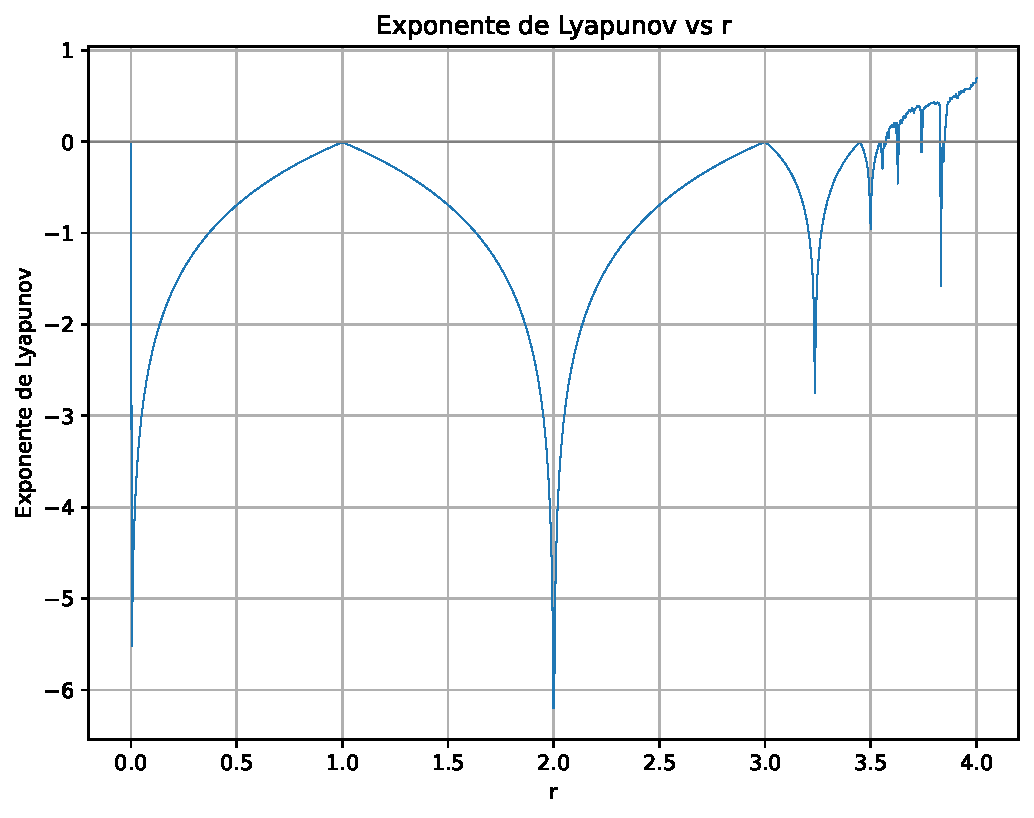
\includegraphics[keepaspectratio]{01-logistica/lyapunov_files/figure-pdf/cell-10-output-1.pdf}
  \caption{Cálculo del coeficiente de Lyapunov para todo el mapa logístico}
\end{figure} 

Vamos a interpretar esta gráfica, y ver si cuadra con los conocimientos
previos del mapa logístico.

Para valores \textbf{\(0 < r \le 1\)}, sabemos que todas las iteraciones
convergen al punto fijo \(x^* = 0\). Por lo tanto el exponente de
Lyapunov: \(\lambda(r) < 0\) ya que no estamos en la zona caótica.

Para \(r = 1\), la ecuación del mapa logístico es \[
   x_{n+1} \;=\; 1 \cdot x_n \,(1 - x_n) \;=\; x_n \,(1 - x_n).
   \]

Los puntos fijos (soluciones de \(x^* = x^*(1 - x^*)\)) se determinan
resolviendo \[
   x^* = x^*(1 - x^*) 
   \quad\Longrightarrow\quad
   x^*(1 - (1 - x^*)) = 0 
   \;\Longrightarrow\;
   x^* \bigl(1 - 1 + x^*\bigr) = 0 
   \;\Longrightarrow\;
   x^* \cdot x^* = 0.
   \]

Por tanto, el único punto fijo es \[
   x^* = 0.
   \]

La derivada del mapa general es \[
   f'(x) = r\,(1 - 2x).
   \]

Si evaluamos en \(r = 1\) en el punto fijo \(x^* = 0\), obtenemos \[
   f'(x^*) \;=\; 1 \cdot \bigl(1 - 2 \cdot 0\bigr) \;=\; 1.
   \]

Es decir, las iteraciones siempre terminan en una derivada igual a 1,
cuyo logaritmos es cero. Por eso el coeficiente de Lyapunov promediado
es cero.

Para valores \textbf{\(1 < r < 3\)}, vemos que de nuevo el exponente es
negativo. En esta zona la función logística tiende a valores estables
comprendidos entre 0 y 1, pero ni es caótica ni periódica. Podemos verlo
matemáticamente, ya que sabemos que en esta zona el mapa logístico
tiende al punto fijo \(1-1/r\), y si evaluamos la derivada de la función
logística en ese punto fijo tenemos \(2 - r\), y como \(1<r<3\) se tiene
\(-1 < 2 - r < 1\), de modo que \(|2 - r|<1\) y por tanto
\(\lambda(r) = \ln|2 - r| < 0\). Es decir, se suman logaritmos que son
siempre negativos, por lo que el promedio final nunca podrá ser
positivo.

Para \(r = 3\) sabemos que el mapa logístico tiende a \[
   x^* \;=\; 1 - \frac{1}{3} \;=\; \frac{2}{3}.
   \]

Evaluándola la derivada en este punto \(x^* = \tfrac{2}{3}\) para
\(r = 3\): \[
   f'\bigl(x^*\bigr) 
   = 3 \cdot \Bigl(1 - 2 \cdot \tfrac{2}{3}\Bigr) 
   = 3 \cdot \Bigl(1 - \tfrac{4}{3}\Bigr) 
   = 3 \cdot \Bigl(-\tfrac{1}{3}\Bigr) 
   = -1.
   \]

Que en valor absoluto es 1, y por lo tanto al igual que el caso con
\(r=1\), el exponente de Lyapunov es cero.

Para \textbf{\(3 < r < r_2 \approx 3.4495\)} sabemos que existe un ciclo
estable de periodo 2. \(\lambda(r)\) en este rango vuelve a ser
negativo, porque aunque ya no convergemos a un punto fijo, sí converge a
un ciclo de periodo 2. En el límite \(r \to r_2\), \(\lambda(r)\) se
acerca nuevamente a 0, pues se produce la segunda bifurcación hacia un
ciclo de periodo 4.

En todos los ciclos restantes hasta \(r_\infty \approx 3.5699456\dots\)*
tenemos el mismo comportamiento, valores negativos en las zonas de los
ciclos y acercándose a cero cuando cambiamos de periodo.

Para \(r_\infty < r \le 4\)** vemos que en la mayoría de estos \(r\) en
los que sabemos que el sistema es caótico se cumple que
\(\lambda(r) > 0\). Sin embargo, dentro de este intervalo caótico
aparecen ``ventanas'' periódicas (por ejemplo, cerca de
\(r\approx 3.8284\), donde hay un ciclo de periodo 3). En esas ventanas
periódicas \(\lambda(r)\) vuelve a ser negativo. Justo en el borde de
cada ventana periódica (bifurcaciones dentro del caos) se tiene
\(\lambda(r)=0\). En la vecindad de \(r = 4\), el valor promedio exacto
es \(\lambda(4) = \ln 2 \approx 0.6931\) tal y como habíamos visto.

\chapter{El exponente de Lyapunov y el
caos}\label{el-exponente-de-lyapunov-y-el-caos}

En la siguiente gráfica vemos lo que hemos ido contando
pormenorizadamente en la sección anterior. Cada vez que el sistema está
en una zona no caótica, el exponente de Lyapunov es negativo.

\begin{figure}[h]
  \centering
  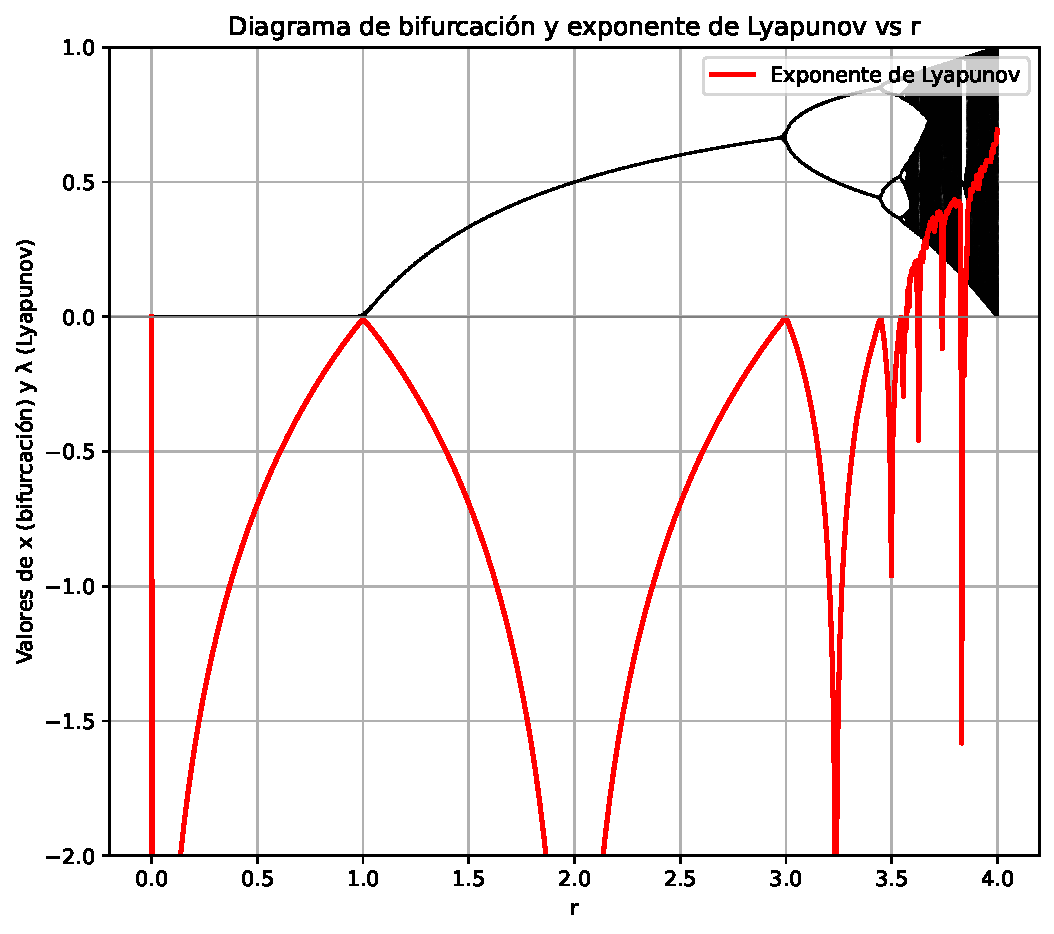
\includegraphics[keepaspectratio]{01-logistica/criterio_files/figure-pdf/cell-2-output-1.pdf}}
  \caption{Diagrama de bifurcación y exponente de Lyapunov en función de $r$}
\end{figure}


De hecho, si hacemos zoom en la zona donde aparece el caos, vemos que en
las ventanas de periodicidad el exponente de Lyapunov se vuelve
negativo.

\begin{figure}[h]
  \centering
  \includegraphics[keepaspectratio]{01-logistica/criterio_files/figure-pdf/cell-3-output-1.pdf}
  \caption{Diagrama de bifurcación y exponente de Lyapunov en función de $r$ (zoom)}
\end{figure}



La pregunta que debemos hacer es la siguiente, \textbf{¿es el exponente
de lyapunov un indicador que nos puede decir si una serie temporal que
estamos observando es caótica?} Una serie temporal es simplemente una
lista de valores que varían con el tiempo, como por ejemplo la
temperatura diaria de una ciudad: \(T_0, T_1, T_2, \dots\).

Llamamos a esos valores \(x_0, x_1, x_2, \dots\) y cada subíndice indica
la ``etapa'' o ``momento'' en que lo medimos.

Decir que una serie temporal es \textbf{caótica} significa, de acuerdo a
la teoría del caos, que ha de cumplir tres condiciones:

\begin{enumerate}
\def\labelenumi{\arabic{enumi}.}
\tightlist
\item
  \textbf{Es determinista}: existe una ``regla'' (una función) que, dado
  el estado actual \(x_n\), calcula el siguiente \(x_{n+1}\). No hay
  azar puro: si conoces \(x_n\) exactamente, sabes \(x_{n+1}\).\\
\item
  \textbf{Tiene sensibilidad a condiciones iniciales}: dos valores muy
  parecidos \(x_0\) y \(x_0 + \delta_0\) se separan de forma exponencial
  a medida que iteras la regla. Aunque \(\delta_0\) sea minúsculo, al
  cabo de varias iteraciones la diferencia es muy grande.\\
\item
  \textbf{Se ve impredecible a largo plazo}: aunque la regla sea
  determinista, al crecer las diferencias ``desordenadas'' parece un
  comportamiento aleatorio.
\end{enumerate}

Por ejemplo, ir anotando los números que salen directamente de una
ruleta no es una serie caótica, ya que no hay ninguna regla para saber
\(x_{n+1}\) si conoces \(x_n\) exactamente. Eso a pesar de ser
impredecible a largo plazo. Es muy importante hacer notar, que un
sistema caótico tiene unas reglas deterministas muy claras. En este caso
\textbf{no se puede calcular ningún exponente de Lyapunov} porque no hay
función \(f\) continua o diferenciable que escriba \(x_{n+1} = f(x_n)\).
Si intentáramos ``forzar'' un cálculo, estaríamos midiendo ruido y
obtendríamos resultados sin sentido práctico: un ``valor de
\(\lambda\)'' aquí no nos dice nada sobre determinismo o caos, sino solo
sobre la aleatoriedad de los datos.

Otro ejemplo de sistemas que no cumple estas premisas es la bolsa. A
todo el mundo le parece que predecir el valor de una acción a lo largo
del tiempo es muy complejo, pero ¿es caótico?. Para ello veremos como
funciona la bolsa. El precio de una acción o de un índice bursátil
depende de decenas de variables:\\
• Resultados financieros de las empresas.\\
• Noticias económicas o políticas.\\
• Sentimiento de los inversores y rumores.\\
• Tipos de interés, inflación, datos macroeconómicos.\\
• Eventos inesperados (crisis, pandemias, etc.).

Cada día (o incluso cada minuto) entran al mercado miles de órdenes de
compra y venta, influidas por estas variables.

No existe una regla sencilla \(x_{n+1} = f(x_n)\). A diferencia del mapa
logístico, donde si conocemos \(x_n\) y el parámetro \(r\) podemos
calcular \(x_{n+1} = r\,x_n\,(1 - x_n)\), en la bolsa no hay una función
sencilla y fija que relacione el precio de hoy con el de mañana.

Por estas razones, el precio de la bolsa es, en gran medida, un proceso
aleatorio que incorpora ruido y reacciones humanas, no un sistema
determinista como el mapa logístico.

Volviendo a la pregunta original. \textbf{¿es una condición necesaria y
suficiente para que una serie sea caótica que su exponente de Lyapunov
sea positivo?}

De acuerdo a la investigación bibliográfica realizada, un
\textbf{exponente de Lyapunov mayor} \(\lambda_{\max} > 0\) es
\textbf{condición necesaria} para que un sistema determinista sea
caótico, pero \textbf{no basta por sí solo} para garantizar caos en
sentido completo.

Un sistema se considera \textbf{caótico} si cumple, entre otros, el
criterio de \textbf{sensibilidad a condiciones iniciales}: dos
trayectorias iniciadas en puntos arbitrariamente próximos se separan
exponencialmente con el tiempo. El \textbf{exponente de Lyapunov}
\(\lambda_{\max}\) mide justamente ese crecimiento (o decrecimiento)
exponencial promedio de una pequeña desviación. Si
\(\lambda_{\max} < 0\), todas las pequeñas diferencias se contraen, y el
sistema converge a un punto fijo o a un ciclo periódico estable:
\textbf{no hay caos}. Por lo tanto, \textbf{tener \(\lambda_{\max} > 0\)
es condición necesaria} para hablar de caos determinista

Aunque \(\lambda_{\max} > 0\) garantiza sensibilidad exponencial, para
que un sistema sea considerado caótico \textbf{en el sentido matemático
completo} también se requiere cumplir otras condiciones mas específicas,
que no citaré en este texto por estar muy por encima de mi nivel. La
explicación larga para el lector interesado se haya aquí:

-- ``The short answer is `No'. As reflected in many of the other posted
responses, positive Lyapunov exponents, by themselves, do not always
indicate `chaos'. Additional information about the system \ldots{} needs
to be performed to conclusively diagnose `chaos' in most systems.''\\
Fuente:
\url{https://www.researchgate.net/post/Does-positive-Lyapunov-exponent-always-mean-chaos}

Sin embargo, en la \textbf{práctica experimental o de series temporales
reales}, suele aceptarse que si la estimación de \(\lambda_{\max}\)
resulta positiva y se ha verificado que:

\begin{itemize}
\tightlist
\item
  El sistema es determinista (o modelado por un conjunto de ecuaciones
  conocidas).\\
\item
  La variable observada permanece en un rango acotado
\item
  Al simular o analizar la trayectoria, no se observan comportamientos
  puramente periódicos ni divergencias triviales.
\end{itemize}

Entonces, \textbf{la probabilidad de que el sistema sea caótico es muy
alta}. Varios autores y estudios confirman que, bajo condiciones
razonables de ruido controlado, un \textbf{exponente de Lyapunov
positivo} es \textbf{una señal muy confiable de caos determinista}.

-- ``The Largest Lyapunov Exponent (LLE) has been frequently used to
investigate presence of chaotic behavior as well as nonlinear
characteristics of time series.''\\
Fuente:
\url{https://www.sciencedirect.com/topics/engineering/largest-lyapunov-exponent}

Aunque \textbf{en teoría} hay que cumplir dos condiciones adicionales,
\textbf{en la práctica}, sobre todo en áreas aplicadas (física
experimental, meteorología, etc.), \textbf{una \(\lambda_{\max}\)
positiva suele considerarse como ``casi certeza'' de caos} siempre que
los cálculos se hayan hecho con series suficientemente largas y con
ruido controlado.

\section{Horizonte de
predictibilidad}\label{horizonte-de-predictibilidad}

¿Por qué es tan importante el exponente de Lyapunov al hablar de
sistemas caóticos?. Para ver su importancia vamos a introducir un
término muy importante, el horizonte de predictibilidad.

El \textbf{horizonte de predictibilidad} es el tiempo máximo durante el
cual podemos hacer predicciones fiables de un sistema caótico, dadas
unas condiciones iniciales con cierta incertidumbre. Aunque conozcamos
la regla determinista que rige el sistema, la sensibilidad a las
condiciones iniciales (medida por el exponente de Lyapunov) impone un
límite práctico a nuestra capacidad de predicción.

En un sistema caótico, dos trayectorias que empiezan muy cerca divergen
de forma \textbf{exponencial}. Si la separación inicial entre ellas es
\(\delta_0\), tras un tiempo \(t\) la separación será aproximadamente

\begin{equation}
\delta(t) = \delta_0\,e^{\lambda_{\max}\,t},
\end{equation}

donde \(\lambda_{\max}\) es el \textbf{exponente de Lyapunov máximo},
que mide la rapidez de esa divergencia.

¿Cuándo ``fracasa'' la predicción?

Definimos un \textbf{umbral de error} \(\Delta\): cuando la divergencia
\(\delta(t)\) alcance \(\Delta\), consideramos que la predicción ya no
es útil. Por ejemplo, si medimos temperatura, \(\delta_0\) podría ser la
imprecisión inicial y \(\Delta\) el error máximo tolerable.

Buscamos el tiempo \(T_p\) tal que

\begin{equation}
\delta(T_p) = \Delta.
\end{equation}

Para derivar de la fórmula partimos de\\
\[
   \delta(T_p) = \delta_0\,e^{\lambda_{\max}T_p} = \Delta
   \]

Luego despejamos \(T_p\):\\
\[
   e^{\lambda_{\max}T_p} = \frac{\Delta}{\delta_0}
   \] \[
   \lambda_{\max}T_p = \ln\!\Bigl(\tfrac{\Delta}{\delta_0}\Bigr)
   \] \[
   \boxed{T_p = \frac{1}{\lambda_{\max}}\,\ln\!\Bigl(\tfrac{\Delta}{\delta_0}\Bigr)}
   \]

¿Cuál es el significado de cada término?

\begin{itemize}
\tightlist
\item
  \textbf{\(\lambda_{\max}\)}: mayor exponente → predicciones válidas
  por menos tiempo.\\
\item
  \textbf{\(\delta_0\)}: si reducimos la imprecisión inicial, alargamos
  \(T_p\).\\
\item
  \textbf{\(\Delta\)}: cuanto más tolerante seas al error, más tiempo
  «aguanta» la predicción.
\item
  Un sistema con \(\lambda_{\max}<0\) tendría, en cambio, un horizonte
  de predictibilidad infinito, pues los errores se contraen y la
  predicción mejora con el tiempo.
\end{itemize}

\textbf{Ejemplo práctico:}\\
En la atmósfera se observa a menudo un exponente\\
\[
\lambda_{\max} \approx 0{,}8\ \text{día}^{-1}.
\]

Además, la \textbf{incertidumbre inicial} realista en modelos y medidas
es más alta, por ejemplo\\
\[
\delta_0 = 10^{-3}\ \text{(°C)},
\]\\
y mantenemos el \textbf{error tolerable}\\
\[
\Delta = 1\ \text{°C}.
\]

Entonces,

\begin{equation}
T_p
= \frac{1}{0.8}\,\ln\!\Bigl(\tfrac{1}{10^{-3}}\Bigr)
=1{,}25 \times \ln(10^3)
=1{,}25 \times 6{,}91
\approx 8{,}6\ \text{días}.
\end{equation}

Este cálculo \textbf{coincide} con el límite práctico de \textbf{7--10
días} que vemos hoy en los pronósticos meteorológicos fiables. El lector
puede echar un vistazo al siguiente artículo:

https://www.stratumfive.com/climate/weather-forecasting-and-chaos-theory/

Aquí se habla de un horizonte de predictibilidad para el tiempo de 8 a
10 días. La cuestión es que por lo aprendido en este proyecto, éste
límite es una barrera que no vamos a poder superar. Si bien en los
últimos 50 años se ha producido un formidable incremento de la precisión
con la que hacemos las predicciones, pasando de predicciones fiables a
un día a tener buenas predicciones a 5 días, el llegar a batir este
límite dos semanas va a ser imposible.

Y hablando de horizontes de predictibilidad, ¿qué te parece el escuchar
que el sistema solar tiene un horizonte de predictibilidad de unos 5
millones de años?. Si Newton levantase la cabeza. Es decir, a pesar de
que tenemos esa preciosa fórmula de la gravitación universal, que
funciona tan bien, su propagación hacia el futuro, cuando tenemos en
cuenta los planetas que componen el sistema solar, deja de ser válida a
4 millones de años vista, que en términos cósmicos es poco tiempo. Y es
que no solamente tenemos errores iniciales, al no poder tener en cuenta
todos los pequeños objetos que vagan por el sistema solar, sino porque
el sistema es inherentemente caótico. De hecho, tal y como anticipó
Poincare, el movimiento de tres cuerpos en el vacío sujetos a sus
respectivas fuerzas de atracción gravitatoria, es ya un sistema caótico,
y que presenta un exponente de Lyapunov positivo en determinadas
circunstancias.

\subsection{Referencias principales}\label{referencias-principales}

\begin{enumerate}
\def\labelenumi{\arabic{enumi}.}
\tightlist
\item
  Wikipedia. ``Chaos theory.''\\
  \url{https://en.wikipedia.org/wiki/Chaos_theory}\strut \\
\item
  ResearchGate. ``Does positive Lyapunov exponent always mean chaos?''\\
  \url{https://www.researchgate.net/post/Does-positive-Lyapunov-exponent-always-mean-chaos}\strut \\
\item
  Wikipedia. ``Butterfly effect.''\\
  \url{https://en.wikipedia.org/wiki/Butterfly_effect}\strut \\
\item
  ScienceDirect Topics. ``Largest Lyapunov Exponent.''\\
  \url{https://www.sciencedirect.com/topics/engineering/largest-lyapunov-exponent}
\end{enumerate}

\part{El Caos en vivo: El péndulo doble}

\chapter{El Péndulo Doble}\label{el-puxe9ndulo-doble}

\section{Introducción}\label{introducciuxf3n-3}

El péndulo doble es quizás uno de los sistemas físicos más estudiados en
el ámbito de la teoría del caos. Esto es debido a que tiene unas
ecuaciones deterministas muy bien conocidas, y a la contraposición con
el péndulo simple. Es decir, mientras que en el péndulo simple con unas
ecuaciones relativamente más sencillas podemos predecir ``ad infinitum''
la posición y velocidad del péndulo, en el caso del péndulo doble, que
no son más que dos péndulos sencillos acoplados, no podemos predecir más
allá de unos pocos segundos.

Dicho de otra manera, un péndulo simple, como el que estudió Galileo, es
un sistema que encaja perfectamente en la mecánica clásica y que se
comporta de una forma determinista, mientras que un péndulo doble tiene
un comportamiento imposible de predecir tras unos pocos segundos. Ambos
están regidos por las mismas leyes de la física, y el péndulo doble es
ligeramente más complejo, pero su comportamiento es totalmente
impredecible. Todo ello a pesar de tener unas ecuaciones que describen a
la perfección su comportamiento.

El análisis matemático de ambos sistemas, el péndulo simple y doble, se
puede obtener en muchas referencias, por ejemplo en
\url{https://paginaspersonales.unam.mx/app/webroot/files/4554/Publica_20190605182303.pdf}.
El análisis matemático del péndulo doble está muy por encima del nivel
de bachillerato.

Sin embargo podemos recurrir a la simulación y experimentación real para
analizar su comportamiento. Empezaremos por realizar simulaciones y
comprobar en el ordenador como se comporta el péndulo doble. Pero, ¿no
resulta muy complicado hacer la simulación de un péndulo doble?. ¿Acaso
no habría que implementar las ecuaciones del péndulo doble, que resultan
realmente complicadas de analizar matemáticamente?. Tenemos dos
soluciones para ello:

\begin{itemize}
\tightlist
\item
  Podemos utilizar simuladores de física como Algodoo
  \url{https://www.algodoo.com/}
\item
  Podemos pedirle a ChatGPT que nos haga una simulación en Python.
\end{itemize}

En este proyecto, he optado por la segunda alternativa, y los resultados
han sido espectaculares. Usando uno de los modelos más avanzados de
OpenAI, el mini4-high, la codificación resultó directa y sin errores.
Copiando el código generado, y ejecutándolo desde mi ordenador pude
tener en unos pocos minutos las simulaciones listas para su interpretación.  

\chapter{Sensibilidad a las condiciones
iniciales}\label{sensibilidad-a-las-condiciones-iniciales}


\section{Descripción General}\label{descripciuxf3n-general}

En esta entrada se analiza un programa escrito en Python para simular y
dibujar \(10.000\) péndulos dobles simultáneamente. El objetivo
principal de la simulación es mostrar la \textbf{sensibilidad a las
condiciones iniciales}, un rasgo característico de los sistemas
caóticos. Cada péndulo comienza con un ángulo inicial ligeramente
distinto para ilustrar cómo pequeñas variaciones pueden dar lugar a
comportamientos muy diferentes a lo largo del tiempo. Es decir, como
verás en el próximo vídeo los péndulos al ser lanzados parecen estar
todos en la misma posición, pero a medida que vamos avanzando en la
simulación se separan totalmente.

\begin{figure}[h]
  \centering
  \scalebox{0.7}{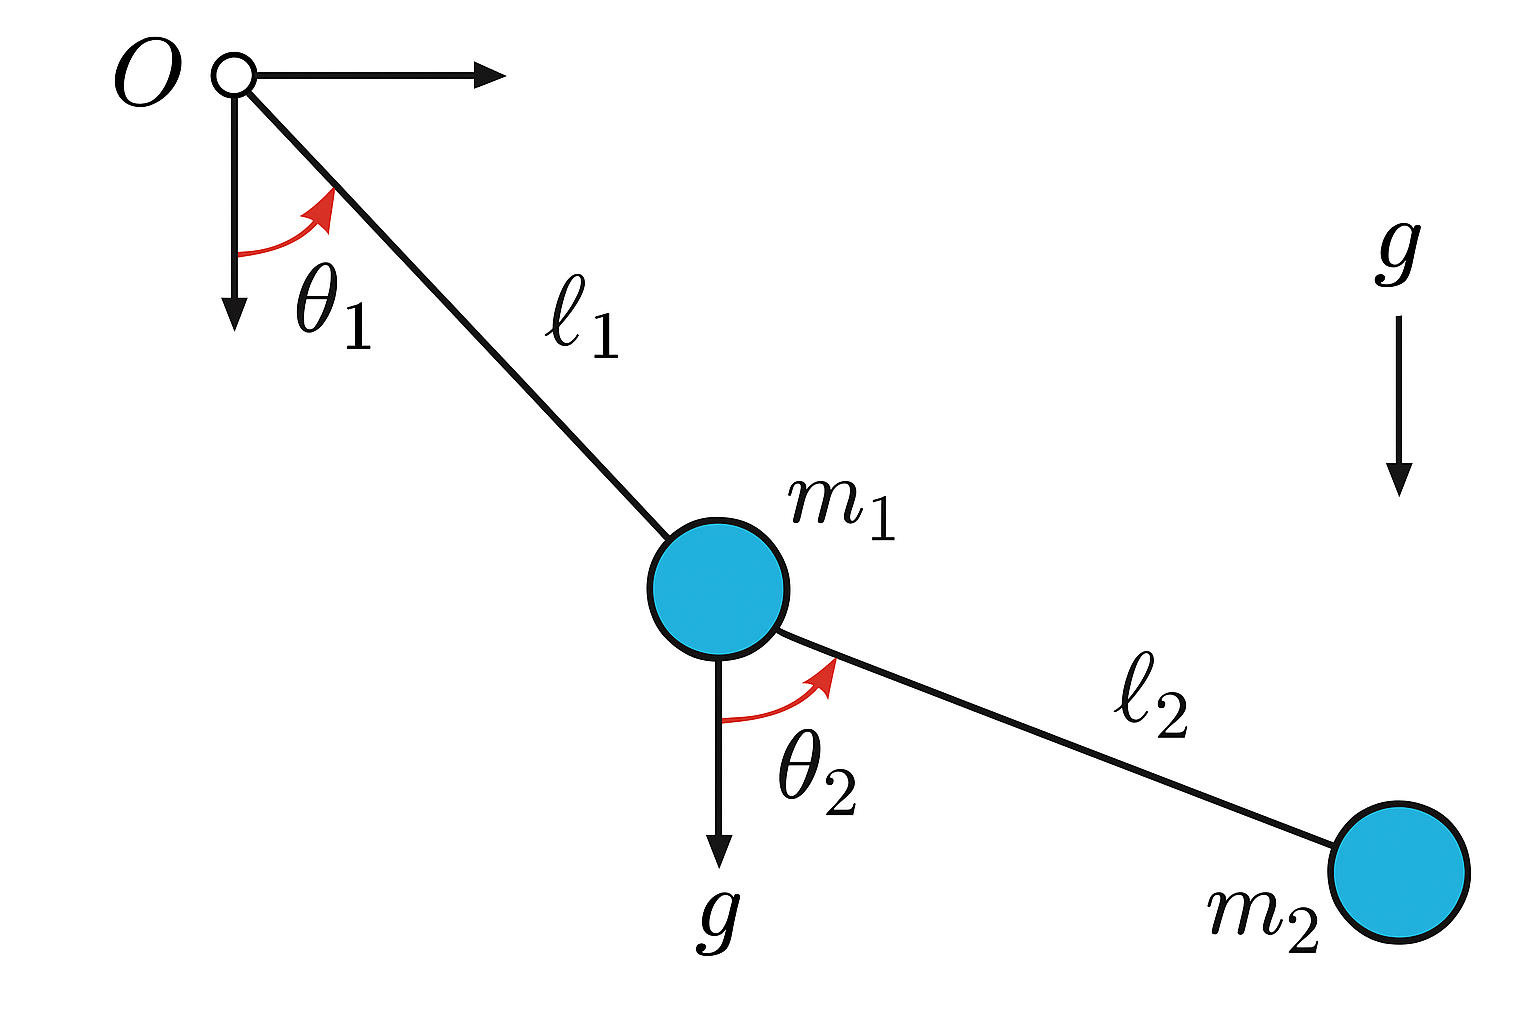
\includegraphics{02-pendulo-doble/PenduloDoble.png}}
  \caption{Esquema del doble péndulo}
\end{figure}



\section{Preparación del Código con
ChatGPT}\label{preparaciuxf3n-del-cuxf3digo-con-chatgpt}

Este código fue \textbf{generado mediante ChatGPT}, aprovechando la
capacidad del sistema para programar en Python. A continuación, se
describe el \emph{prompt} que dio origen a esta simulación:

\begin{quote}
\textbf{Prompt sugerido:}\\
``Genera un código en Python que utilice Python para simular \(10000\)
péndulos dobles al mismo tiempo. Cada péndulo debe tener la primera pata
en la misma posición (170 grados) y la segunda pata con un ángulo
inicial también de 170 grados pero ligeramente distinto en cada péndulo,
espaciado uniformemente entre 170 y 170.1 grados. El objetivo es
visualizar la sensibilidad a las condiciones iniciales superponiendo
todos los péndulos en una misma imagen. Dibuja cada péndulo de un color,
y muestra la animación en tiempo real. Mi ordenador dispone de una
tarjeta gráfica Nvidia y tengo instalado CUDA, así que úsalo para
acelerar las simulaciones. No tengas en cuenta la fuerza de
rozamiento.''
\end{quote}

Tras varias iteraciones de este prompt, al final conseguí un código que
se ejecutase. La depuración del código es realmente fácil de hacer. Cada
vez que ChatGPT me daba un código, lo corría en el ordenador mediante el
comando ``python programa.py'', y los errores se los alimentaba de
vuelta a ChatGPT que a su vez me devolvía el código depurado.

En el código proporcionado, los parámetros físicos de cada péndulo doble
los ha definido ChatGPT de la siguiente manera:

\begin{itemize}
\item
  \textbf{Longitudes de los brazos}

  \begin{itemize}
  \tightlist
  \item
    Longitud del primer brazo: \(l_1 = 1.0\) metros\\
  \item
    Longitud del segundo brazo: \(l_2 = 1.0\) metros
  \end{itemize}

  En la representación gráfica cada metro es representado a través de
  150 píxeles.
\item
  \textbf{Masas de los cuerpos}

  \begin{itemize}
  \tightlist
  \item
    Masa del primer cuerpo: \(m_1 = 1.0\) Kg
  \item
    Masa del segundo cuerpo: \(m_2 = 1.0\) Kg
  \end{itemize}

  La gravedad es la terrestre, \(9.81 Kg/m^2\). El péndulo simulado es
  grande, pero lo bueno de hacerlo grande es que va mas lento en tiempo
  que un péndulo pequeño, por lo que su movimiento se aprecia mejor en
  la simulación. El péndulo oscila sin parar ya que no hemos puesto
  ninguna fuerza de rozamiento.
\end{itemize}

\section{Vídeo con la simulación}\label{sec-abanico}

Una vez preparado el código procedía a correrlo y grabar la ventana de
salida en un archivo de vídeo que se encuentra a continuación. Hay que
tener en cuenta que el código Python generado por ChatGPT, avanza en
pasos de 1 milisegundo de tiempo real, y que debido a la gran cantidad
de péndulos la simulación no llega a ser en tiempo real. Por eso le
pedía a ChatGPT que incluyera un texto en la simulación que mostrase el
tiempo real durante la simulación.

El lector interesado puede ver el video en el siguiente enlace \url{https://colacaos.github.io/ColaCAOS/02-pendulo-doble/Pendulumabanico.mp4}

El resultado es sorprendente e hipnotizante. ¿Como puede ser que
péndulos que se lanzan tan cercanos diverjan tan rápidamente?. Si
observamos atentamente el vídeo hasta el segundo 1 de la simulación
todos los péndulos van casi al unísono. En el segundo 2, que es cuando
llegan al otro extremo, vemos que el ``abanico'' ya se empieza a abrir.
Y en la bajada que le sigue se desata el caos. Del segundo 2 al tres ya
estamos con una divergencia total, y a partir de ahí cada uno va a su
bola, ¡caos total!.

\begin{figure}[h]
  \centering
  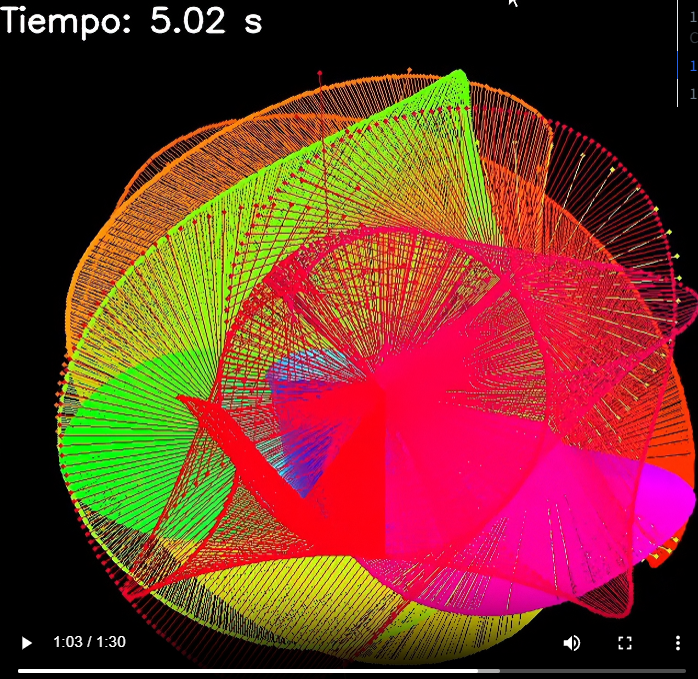
\includegraphics[width=0.9\textwidth]{02-pendulo-doble/abanico.png}
  \caption{Segundo número 5 de la simulación (10.000 pendulos separados inicialmente 10 microgrados)}
\end{figure}

Ahora reflexionemos. Péndulos que fueron lanzados con diferencias de
milésimas de grado, tienen trayectorias que divergen enormemente tras 5
segundos. ¿Acaso es éste un sistema físico que cuyo comportamiento
podamos predecir en la vida real?. Pues yo diría que no. Nos enfrentamos a dos problemas en la realidad:

\begin{itemize}
\tightlist
\item
  No podemos medir con total exactitud el estado inicial de nuestro
  sistema
\item
  No podemos simular los modelos matemáticos con una precisión infinita
  en un ordenador
\end{itemize}

\chapter{Mapa de Fases}\label{mapa-de-fases}

Recordemos que durante el estudio de la función logística, el diagrama
de bifurcación aparecía una y otra vez cada vez que hacíamos zoom en una
zona pequeña de \(r\). Veíamos la misma estructura repetida en zonas de
\(r\) cada vez más pequeñas. ¿Pasará algo similar con el péndulo doble?.
Vamos a ir paso a paso.

En primer lugar, vamos a simular 36 x 36 péndulos, cada uno de ellos con
diferentes condiciones iniciales de los dos brazos. Puesto que cada uno
de los ángulos puede tomar 360 grados, vamos a repartirlos en 36
posiciones diferentes cada uno de ellos desde 0,10,20 .. hasta 350
grados. Obviamente, aquí están separados bastante por lo que su
evolución va a ser diferente.

Por lo tanto estamos viendo 1296 péndulos dobles al mismo tiempo! Cada
uno en su pequeña celda de 20×20 píxeles, todos organizados en una
cuadrícula de 36×36. El resultado es una imagen de 720×720 donde cada
cuadradito muestra un péndulo doble distinto, lanzado con ángulos
iniciales que varían sistemáticamente en filas y columnas.

Cada celda se trata como un único péndulo doble, con los mismos
parámetros que en el caso del abanico de péndulos (masas \(m_1=m_2=1\),
longitudes \(l_1=l_2=1\), gravedad \(g=9.81\)).

Se dibujan las líneas de los brazos en blanco y los tres puntos de unión
en colores rojo, verde y azul para los pivotes, la primera masa y la
segunda masa respectivamente.

Con cada iteración, la simulación avanza y se pinta el estado
actualizado, de modo que se ve un baile de péndulos distintos en cada
casilla.

\section{Prompt para Generar Este Script con
ChatGPT}\label{prompt-para-generar-este-script-con-chatgpt}

\begin{quote}
\textbf{Prompt para la generación del código}\\
``Quiero un código en Python para mi tarjeta Nvidia y Cuda para simular
una \textbf{cuadrícula 36×36 de péndulos dobles} en paralelo. Cada celda
debe inicializar su péndulo con un ángulo para el primer brazo
comprendido entre 0 y 350 grados en pasos de 10 grados, y con un ángulo
para el segundo brazo comprendido entre 0 y 350 grados en pasos de 10
grados. Utiliza los siguientes parámetros de simulación para los
péndulos (\(m_1 = m_2 = 1\), \(l_1 = l_2 = 1\), \(g = 9.81\) y cero
rozamiento).\\
Dibuja cada péndulo en su propia celda de 20×20 píxeles dentro de una
imagen global de 720×720. Dibuja los brazos (longitudes 6 píxeles) en
blanco y los pivotes como círculos pequeños en rojo, verde y azul.
Muestra la ventana en tiempo real y sal al presionar Esc.''
\end{quote}

Al ver la cuadrícula completa, el lector observa cómo cambia el
comportamiento del péndulo doble al variar sus ángulos iniciales en
pequeños pasos de 10°. En la esquina superior izquierda
\((-180^\circ,-180^\circ)\) el movimiento puede ser muy distinto al de
la esquina inferior derecha \((+170^\circ,+170^\circ)\).

Es un ``mapa de fase'' visual: cada casilla revela un patrón dinámico
único, mostrando cómo la mecánica no lineal responde a distintos puntos
de partida. ¿Por qué se llama mapa de fase?. Cuando dibujamos una
función senoidal a lo largo del tiempo, vemos un patrón repetido. Si
pintamos otro seno al lado, con igual amplitud y frecuencia, pero
cambiando el ángulo inicial, veremos el mismo patrón pero desplazado en
el tiempo por ese ángulo inicial. Estamos, por lo tanto, en otra
``fase'' del mismo sistema. Otra forma más cotidiana de verlo es con la
Luna: hablamos de fases para referirnos a la iluminación relativa de la
Luna por el Sol tal y como lo vemos desde la Tierra. Así tenemos fase
creciente, menguante, llena, etc.


\begin{figure}[h]
  \centering
  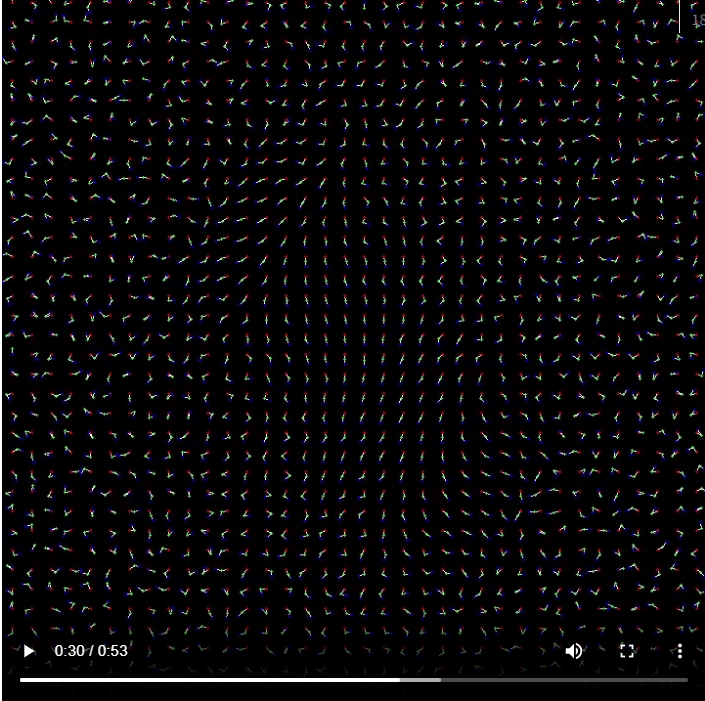
\includegraphics[width=0.9\textwidth]{02-pendulo-doble/mapafases1.png}
  \caption{Estado de 36x36 péndulos dobles tras 30 segundos de simulación}
\end{figure}


De nuevo, animo al lector a ver el vídeo completo en \url{https://colacaos.github.io/ColaCAOS/02-pendulo-doble/MapaFase.mp4}


Vemos una zona central en la que los péndulos parten de ángulos
pequeños. En este caso observamos que el comportamiento es muy similar
al de un péndulo simple. Es, por así decirlo, una zona de estabilidad
del sistema. Pregunté a ChatGPT por qué se produce esta zona de
estabilidad y su respuesta fue la siguiente.

\subsection{Aproximación de Ángulo
Pequeño}\label{aproximaciuxf3n-de-uxe1ngulo-pequeuxf1o}

En la simulación del péndulo doble, cada péndulo tiene dos ángulos
\(\theta_1\) y \(\theta_2\). Cuando ambos son pequeños, la dinámica se
``desacopla'' casi como si fueran dos péndulos simples en serie, pero
sin generar las fuertes interacciones que provocan el caos. Veamos por
qué:

\begin{enumerate}
\def\labelenumi{\arabic{enumi}.}
\tightlist
\item
  Las ecuaciones originales del péndulo doble incluyen términos no
  lineales muy potentes (producto de \(\sin(\theta_1 - 2\,\theta_2)\),
  \(\cos(2\,\delta)\), etc.).\\
\item
  Si \(\theta_1\) y \(\theta_2\) permanecen pequeños, esos términos no
  lineales pierden relevancia: \(\sin(\theta_1)\approx \theta_1\),
  \(\sin(\theta_1 - 2\,\theta_2)\approx \theta_1 - 2\,\theta_2\), y
  \(\cos(2\,\delta)\approx 1\).\\
\item
  Resultado: el sistema casi se comporta como dos péndulos simples que
  oscilan suavemente y de forma \textbf{aproximadamente periódica}. No
  hay ``explosión'' de sensibilidad porque las variaciones pequeñas no
  se amplifican de forma exponencial. Es la zona donde la energía no
  alcanza para explorar el caos.
\end{enumerate}

En otras palabras, en el centro de la ``cuadrícula de fase'' hay un área
donde las trayectorias son estables, casi previsibles, iguales a las que
obtendrías si estudiaras un péndulo simple (o dos acoplados muy
débilmente). Observas oscilaciones regulares, de ida y vuelta, sin
divergencias drásticas.

\subsection{¿Por Qué Llamarlo ``Zona de
Estabilidad''?}\label{por-quuxe9-llamarlo-zona-de-estabilidad}

Cuando hablamos de sistemas dinámicos, llamamos ``estable'' a aquella
región donde las pequeñas perturbaciones no se magnifican con el tiempo.

Si en el experimento gráfico seleccionas solo las celdas centrales,
notarás que los péndulos dobles describen curvas suaves, casi
sinusoidales, muy parecidas a las de un péndulo simple. Esa cohesión de
trayectorias es lo que define la estabilidad: todas las simulaciones de
esa región inicial ``viajan juntas'', sin dispersarse.

\section{Transición hacia el Caos}\label{transiciuxf3n-hacia-el-caos}

A medida que nos alejamos del centro (es decir, cuando comienzas a dar a
\(\theta_1\) o \(\theta_2\) valores más grandes, digamos 30°, 40° o
más), las ecuaciones no lineales cobran protagonismo. Entonces:

\begin{enumerate}
\def\labelenumi{\arabic{enumi}.}
\tightlist
\item
  Los términos \(\sin(\theta)\) ya no son equivalentes a \(\theta\).\\
\item
  Aparecen resonancias internas: la interacción entre el primer y el
  segundo brazo se hace más intensa.\\
\item
  Surge la \textbf{sensibilidad exponencial}: dos péndulos con
  diferencias iniciales de solo unos grados comienzan a divergir
  rápidamente tras pocas oscilaciones.
\end{enumerate}

Así, justo en el borde de esa zona estable, empieza a nacer el caos: las
trayectorias dejan de ser regulares y adquieren formas impredecibles.

Esto nos recuerda a lo que pasaba con la función logística a medida que
crecía \(r\). Hasta \(r=3\) estábamos en una zona muy estable, con un
solo valor final. Ahora el parámetro que controla la estabilidad es el
ángulo desde el que lanzamos el péndulo. Para ángulos pequeños estamos
en zona estable y para ángulos mayores estamos en zonas de caos. En
ambos casos, cuando suministramos más ``energía'' al sistema bien sea en
forma de un mayor \(r\) o un mayor ángulo inicial el sistema se vuelve
caótico.

\section{Mapa de fase detallado}\label{mapa-de-fase-detallado}

Ahora vamos a simular muchísimos más péndulos, para obtener un mapa de
fase mas detallado. Para ello ahora la simulación se organiza en una
cuadrícula de \(720 \times 720\) péndulos. Cada columna \(i\)
corresponde a un ángulo inicial \[
\theta_1(i) \;=\; -\pi \;+\; i\,\frac{2\pi}{719}, 
\quad i = 0,1,\dots,719,
\] y cada fila \(j\) a un ángulo inicial \[
\theta_2(j) \;=\; -\pi \;+\; j\,\frac{2\pi}{719}, 
\quad j = 0,1,\dots,719.
\]

Así, la celda \((i,j)\) arranca con condiciones \[
\theta_1 = \theta_1(i), 
\qquad
\theta_2 = \theta_2(j).
\]

Como cada péndulo es ahora un píxel, ¿cómo podemos visualizar su
estado?. Pues recurrimos a un código de colores. Entonces para cada
péndulo cogemos los angulos \(\theta_1\) y \(\theta_2\) en los que se
encuentra y hacemos una primera normalización. Para cada péndulo se
calculan \[
     n_1 = \frac{\sin(\theta_1) + 1}{2},
     \quad
     n_2 = \frac{\sin(\theta_2) + 1}{2},
   \] de modo que \(n_1,n_2 \in [0,1]\). De esta manera no tenemos
valores negativos del estado, es decir su estado va desde 0 hasta 1.

A continuación promediamos, ambos valores \(n_1\) y \(n_2\) y escalamos
al equivalente de 8 bits, es decir 256 valores, \([0,255]\): \[
     \text{Promedio} = \Bigl(\frac{n_1 + n_2}{2}\Bigr)\times 255.
   \]

Y por último el código generado por ChatGPT aplica un código de colores
al valor promedio resultando en:

azul para valores bajos (\(\approx 0\)),

verde/amarillo para valores intermedios,

rojo para valores altos (\(\approx 255\)).

El resultado de la simulación se puede ver en el siguiente vídeo \url{https://colacaos.github.io/ColaCAOS/02-pendulo-doble/MapaFase.mp4}.

\begin{figure}[h]
  \centering
  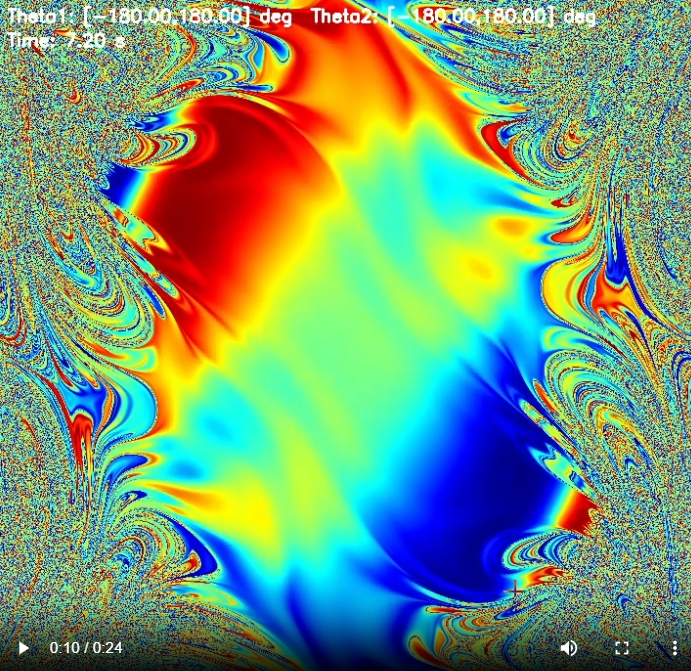
\includegraphics[width=0.9\textwidth]{02-pendulo-doble/mapafases2.png}
  \caption{Mapa de Fase Detallado de 720x720 péndulos}
\end{figure}

Como anticipábamos, en la zona central hay estabilidad, y fuera de ella
no se ven patrones, sino que aparece una especie de ruido. En estas
zonas ``ruidosas'' lo que tenemos es caos, es decir, el estado del
péndulo varía continuamente, y lo que es más importante el estado de
cada péndulo es totalmente distinto de los péndulos vecinos, lo que
manifiesta de nuevo la extrema sensibilidad a las condiciones iniciales.

Para ver más detalladamente esta sensibilidad a las condiciones
iniciales vamos a hacer zooms en áreas alejadas del centro. Se hacen
hasta tres zooms consecutivos hasta llegar a una zona rectangular de
0.01 grados x 0.01 grados en las que se simulan los 720x720 péndulos. No
importa cuanto nos adentramos en el mapa de fase: no se consigue que los
péndulos vecinos vayan a la vez. El vídeo detallado está en \url{https://colacaos.github.io/ColaCAOS/02-pendulo-doble/ZoomSucesivo.mp4}

En el siguiente vídeo \url{https://colacaos.github.io/ColaCAOS/02-pendulo-doble/MapaFaseAcelerado.mp4} aparece la misma simulación, pero esta vez dejando
que corra más el tiempo. En ella se ve que a medida que avanza la
simulación la zona central se va reduciendo, y el caos se apodera de más
zonas. Hay que tener en cuenta que estamos en un sistema sin rozamiento,
y que puede estar corriendo infinitamente. Zonas que al principio
parecían estables, se convierten en caóticas, quedando una pequeña
porción como estable.

Se pueden ver aparecer algunas pequeñas ``islas'' de estabilidad.
Hagamos zoom en una de ellas y veamos como avanza la simulación en ella (vídeo en \url{https://colacaos.github.io/ColaCAOS/02-pendulo-doble/MapaFaseAceleradozoom.mp4}) :

Al igual que en el caso del mapa logístico hay pequeñas zonas de
estabilidad alejadas del centro, rodeadas de caos. Pero la verdad es que
hay que decir que son unos pocos y limitados casos.

\chapter{Bifurcaciones}\label{bifurcaciones}

¿Qué más paralelismos podemos encontrar en el doble péndulo al
compararlo con el mapa logístico?. Vamos a hacer un nuevo ejercicio. En
este caso vamos a simular la diagonal del mapa de fases anterior, es
decir, vamos a coger los valores de \(\theta_1\) y de \(\theta_2\) y
los vamos a variar desde -180 hasta 180 grados simultáneamente por medio
de una sola variable de control. Puesto que el péndulo doble no tiende
hasta un valor final, ya que está continuamente moviéndose al ser sin
rozamiento, vamos a registrar el valor máximo en cada oscilación, y lo
vamos a plotear para cada valor del ángulo inicial. Veamos el resultado:

\begin{figure}[h]
  \centering
  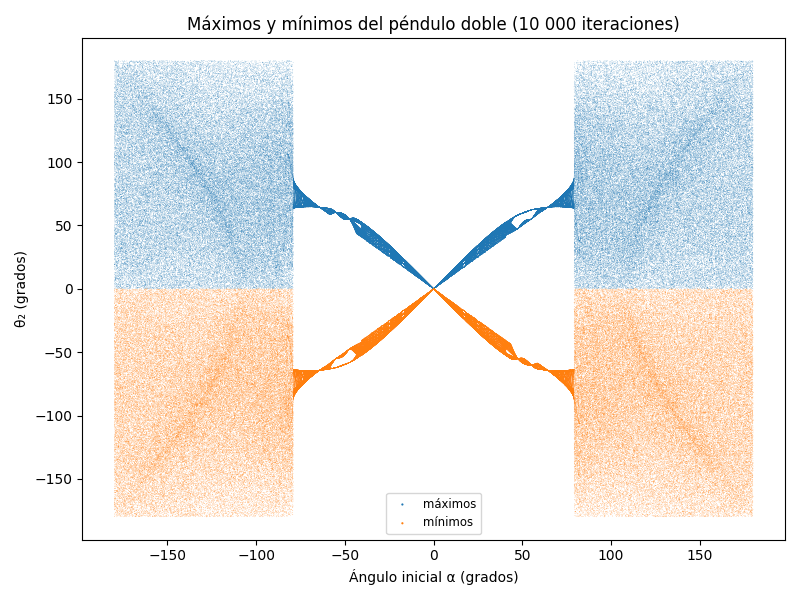
\includegraphics[width=0.9\textwidth]{02-pendulo-doble/BifurcacionesDoble.png}
  \caption{Bifurcaciones en el doble péndulo}
\end{figure}

Vemos tres zonas diferenciadas. La primera de ella de 0 hasta 40 grados.
En esta zona el valor de los máximos alterna entre varios puntos, con
muchas ramificaciones o bifurcaciones adicionales que se van expandiendo
y replegando. En ningún momento podemos hablar de caos, sino de
comportamiento periódico

\begin{figure}[h]
  \centering
  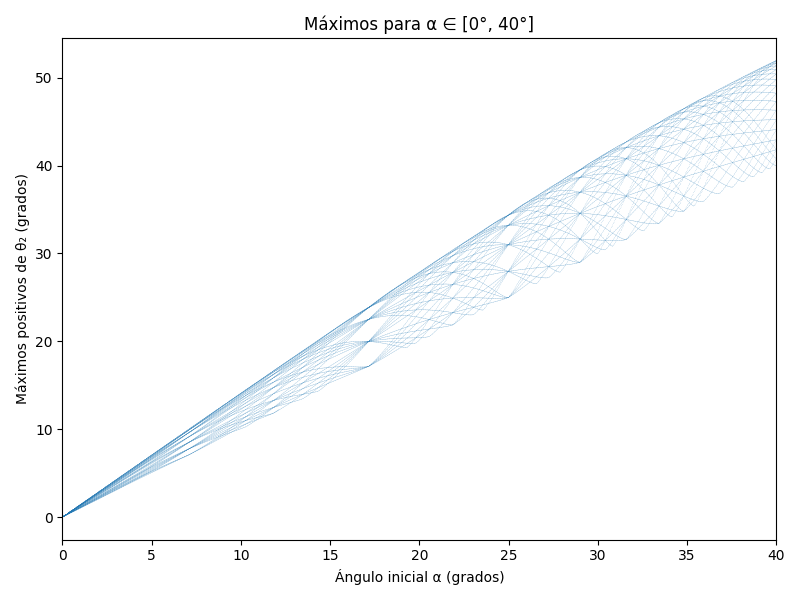
\includegraphics[width=0.9\textwidth]{02-pendulo-doble/BifurcacionesDobleZona1.png}
  \caption{Bifurcaciones en el doble péndulo zoom 1}
\end{figure}


A partir de los 43 grados, el diagrama se abre en dos ramas
perfectamente distinguibles, que se vuelven a juntar a partir de los 57
grados. Curiosamente en torno a 64 grados, tenemos un único punto, por
lo que el sistema podríamos decir que se comporta igual que un péndulo
simple. De 64 grados hasta casi los 80 seguimos con las
ramificaciones/bifurcaciones. Y a partir de los 80 grados tenemos el
caos absoluto.

\begin{figure}[h]
  \centering
  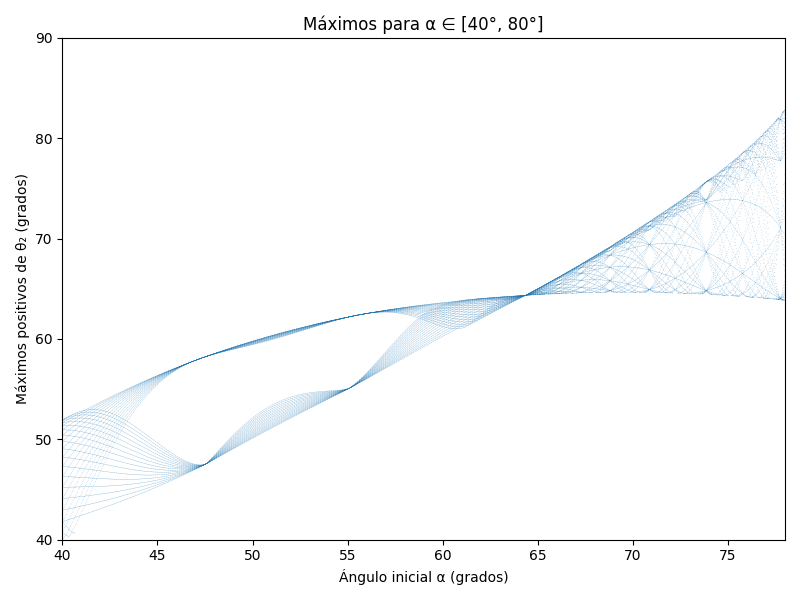
\includegraphics[width=0.9\textwidth]{02-pendulo-doble/BifurcacionesDobleZona2.png}
  \caption{Bifurcaciones en el doble péndulo zoom 2}
\end{figure}



Visto lo visto, me pregunté lo siguiente. ¿Cuál será el exponente de
Lyapunov en cada una de las zonas?. Si bien yo no sabía como calcularlo,
pues a diferencia de la función logística no tengo una expresión para ir
calculando la derivada, le lancé la pregunta a ChatGPT. Al parecer
existe un algoritmo llamado de ``método de Benettin'' que permite
calcularlo. ChatGPT lo implementó en un script de Python y lo lancé en
mi ordenador. El resultado fue el mostrado en la \autoref{fig:BifurcacionesDobleLyapunov}.

\begin{figure}[h]
  \centering
  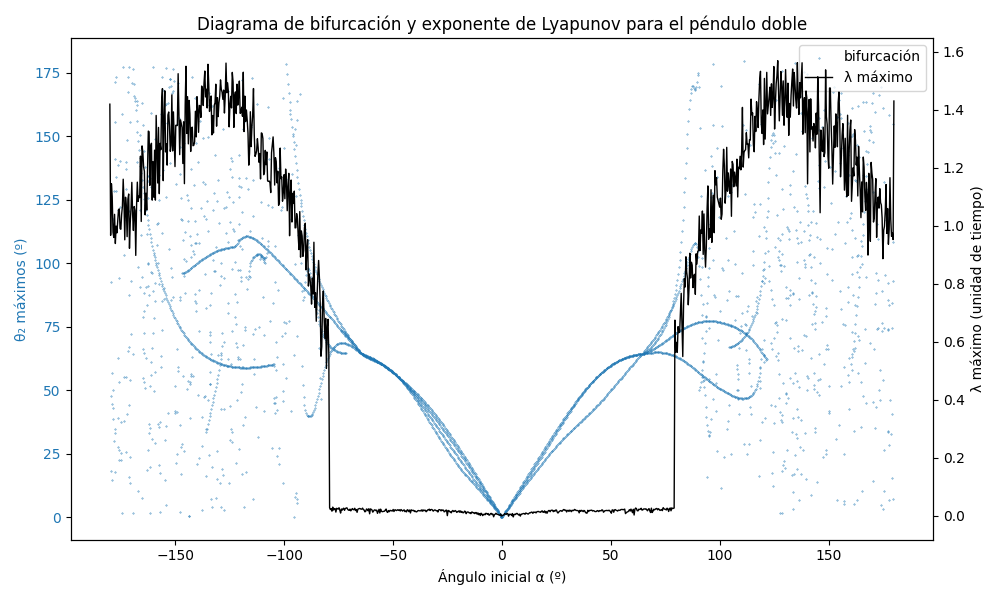
\includegraphics[width=0.9\textwidth]{02-pendulo-doble/Lyapunov.png}
  \caption{Bifurcaciones en el doble péndulo y exponente de Lyapunov}
  \label{fig:BifurcacionesDobleLyapunov}
\end{figure}



Al igual que con la función logística el exponente es prácticamente cero
hasta los 80 grados. A partir de ahí sube abruptamente hasta valores de
más de uno, lo que nos confirma que estamos en una zona caótica.

\section{Zonas estables y caóticas en la
atmósfera}\label{zonas-estables-y-cauxf3ticas-en-la-atmuxf3sfera}

Vamos a extender los paralelismos. Ya hemos visto como dos sistemas
tienen comportamientos parecidos en cuanto a su comportamiento caótico.
Vemos que aparecen bifurcaciones, zonas estables, zonas caóticas, etc..

En meteorología también distinguimos \textbf{regímenes estables},
\textbf{transiciones} y \textbf{comportamiento caótico}, de modo que el
horizonte de predictibilidad varía según el nivel de caos.

Así tenemos zonas de estabilidad atmosférica en determinadas regiones
del planeta, que vienen dadas por lo general por estas situaciones como
los \textbf{Bloqueos atmosféricos}: grandes áreas de alta presión que
pueden persistir días o semanas, desviando borrascas y estabilizando el
tiempo.

En España es el típico anticiclón de las Azores, que cuando se sitúa en
las Azores provoca que no entren las borrascas en la península,
situación que puede llegar a durar varias semanas, y en el que el tiempo
es muy estable.

En estos casos las pequeñas perturbaciones no se amplifican rápidamente
y la predicción puede ser fiable hasta \textbf{8--10 días} o más.

\begin{quote}
Más información sobre bloqueos:\\
url{https://cazatormentas.com/anticiclones-bloqueo-patron-climatico/}
\end{quote}

También hay zonas de alta actividad caótica que se pueden dar por

\begin{itemize}
\tightlist
\item
  \textbf{Convección intensa}: tormentas y cumulonimbos que evolucionan
  en horas.
\item
  \textbf{Frentes rápidos}: líneas de inestabilidad que se reorganizan
  de forma impredecible.
\end{itemize}

Aquí el horizonte de predictibilidad baja a \textbf{1--2 días} o menos,
pues un error pequeño en humedad o temperatura crece exponencialmente.

\chapter{Qué podemos predecir}\label{quuxe9-podemos-predecir}

Hasta ahora nos hemos llevado la impresión de que en un sistema caótico
no podemos predecir nada. Pero tampoco es así la cosa, y lo vamos a ver
con el péndulo doble. Vamos a simular el péndulo doble tirándolo desde
\(\theta_1=170\) grados y \(\theta_2=170\) grados, posición de partida
que sabemos que es caótica. El ángulo \(\theta_2\) lo vamos a variar 20
veces en pasos de 0.0005 grados (en total 1 milésima de grado de
variación). Lanzamos esos 20 péndulos, y le pedimos a ChatGPT que en la
simulación vaya acumulando la distancia total recorrida por cada péndulo
en su extremo. El resultado para los primeros 20 segundos de simulación
está en la siguiente figura:

\begin{figure}[h]
  \centering
  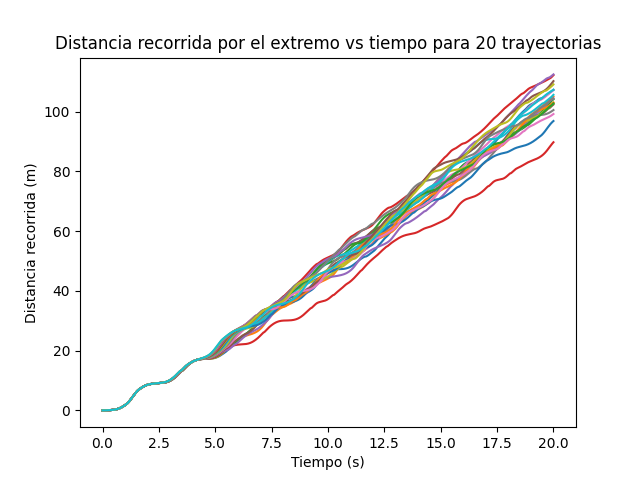
\includegraphics[width=0.9\textwidth]{02-pendulo-doble/Distancia20.png}
  \caption{Distancia recorrida por el extremo del péndulo}
\end{figure}


Como podemos ver la trayectoria de los 20 péndulos diverge desde el
principio en términos de la distancia recorrida, y puesto que estamos
hablando de diferencias de 0.5 milésimas de grado entre péndulos,
sabemos que el predecir la distancia recorrida con exactitud en la
realidad va a ser imposible. Es decir, estamos donde estábamos hasta
ahora.

Pero, ¿qué pasa si simulo 1000 segundos?. Pues como vemos en la
siguiente figura, el sistema ya no parece tan impredecible. La distancia
recorrida va incrementándose prácticamente de forma lineal cuando
ampliamos la duración de la simulación.

\begin{figure}[h]
  \centering
  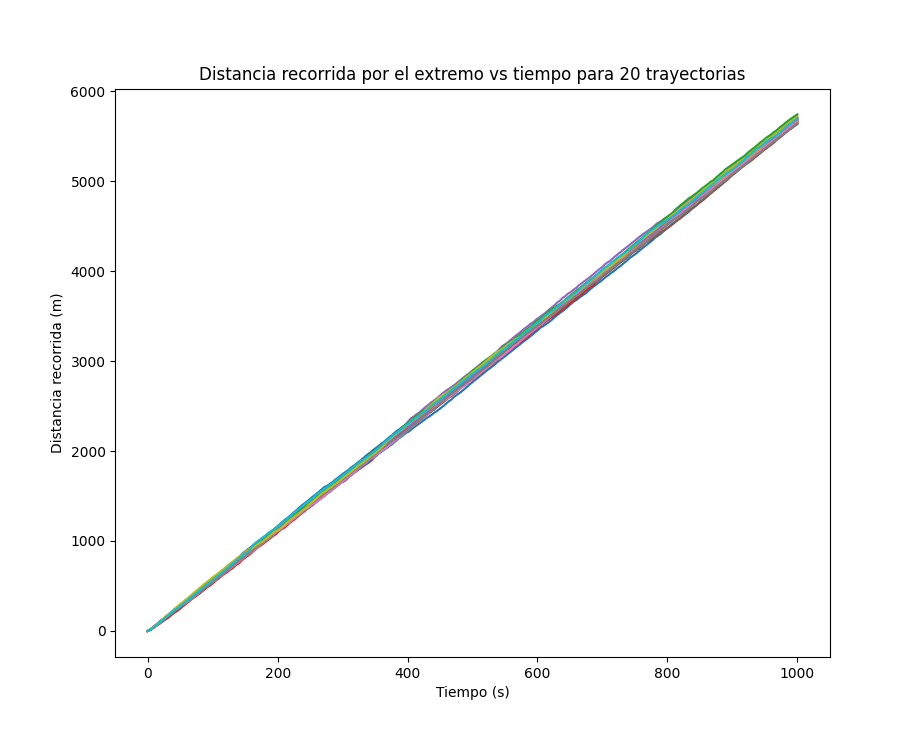
\includegraphics[width=0.9\textwidth]{02-pendulo-doble/Distancia1000.png}
  \caption{Distancia recorrida por el extremo del péndulo tras 1000 segundos}
\end{figure}


Esto es lo que pasa en la predicción climática cuando
hacemos predicciones a largo plazo. Si bien no podemos saber lo que
pasará en un día concreto en un lugar preciso, sí podemos saber su
comportamiento con un margen de error razonable. Al igual que con el
péndulo doble, en el que podemos predecir la distancia recorrida a los
2000 segundos viendo lo que se ha movido en los primeros 1000 segundos:
va a ser aproximadamente el doble sin mucho margen de equivocación.

\section{Ejemplos en predicción
climática}\label{ejemplos-en-predicciuxf3n-climuxe1tica}

Hay varios ejemplos que ilustran como se aplica este principio a la
predicción climática. Sin duda, el ejemplo más ilustrativo es el
\textbf{Predicción de la temperatura media global}. Para ello se usa un
modelo CGM (General Circulation Model), que es un modelo de la
Circulación General de la Atmósfera y los Océanos. Con este modelo,
aunque no sepamos si lloverá en Madrid el 15 de julio de 2030, podemos
proyectar que la temperatura media anual aumente.

Otro ejemplo es el uso de Modelos empíricos combinados con GCMs para
estimar la frecuencia de olas de calor o periodos de sequía en un
horizonte de 10--30 años. Aunque la fecha exacta de la próxima ola de
calor es impredecible, podemos calcular que su probabilidad anual
aumenta de, por ejemplo, un 5 \% a un 15 \% bajo escenarios de +2 °C de
calentamiento global.

La enseñanza clave es que \textbf{el clima} funciona como el
\textbf{comportamiento total a largo plazo} del péndulo doble:\\
- A \textbf{corto plazo}, ambos sistemas son caóticos e impredecibles
con precisión puntual.\\
- A \textbf{largo plazo}, emergen \textbf{tendencias medias} y
estadísticas que sí podemos estimar y utilizar para planificar
políticas, infraestructuras y medidas de adaptación.

Así, la analogía del péndulo doble nos ayuda a entender por qué los
modelos climáticos son fiables para predecir promedios y tendencias,
aunque jamás podrán garantizar el tiempo puntual de un día concreto
dentro de meses o años.

\chapter{Experimentos}\label{experimentos}

\section{Introducción}\label{introducciuxf3n-4}

Para observar y realizar experimentos sobre el caos en un sistema físico
real, he adquirido un péndulo doble, un dispositivo en el que es posible
apreciar el caos con facilidad y en un corto período de tiempo.

En este experimento he comprobado que, en el péndulo doble, los pequeños
errores y las desviaciones de las condiciones iniciales se multiplican
muy rápidamente, de modo que resulta ser un sistema caótico, aunque existan ecuaciones para determinar la posición de cada masa. 

En primer lugar, he colocado tres pegatinas de colores: la roja en el extremo del
segundo péndulo, la verde en el eje que une el primer péndulo con el
segundo y la azul en el eje del primer péndulo. A continuación, mediante
un programa que desarrollé en Python con la ayuda de ChatGPT y una
webcam, he seguido las trayectorias de cada uno de los tres puntos de
color, que corresponden a las partes más relevantes del péndulo doble.
Para reproducir condiciones iniciales prácticamente idénticas, dejé caer
el péndulo siempre desde la vertical ---a 90 grados respecto a la
posición de equilibrio--- , con el segundo péndulo colgando en la misma
orientación que el primero, y lo impulsé cada vez de la manera más suave
posible, únicamente lo necesario para que comenzara a oscilar y
adquiriera la misma velocidad inicial. Repetí este procedimiento varias
veces y registré la trayectoria de los tres puntos coloreados con mi
programa. Posteriormente, elaboré una animación en la que se muestran
las trayectorias del punto rojo ---el que presenta comportamiento más
caótico--- en tiempo más lento que el real, con el fin de apreciar mejor
las diferencias entre cada ensayo. En dicha animación puede observarse
que, a partir del primer segundo, las trayectorias comienzan a divergir
significativamente y, al cabo de unos segundos, resultan completamente
distintas. Lo mismo pasaba en las simulaciones de abanico que vimos en
la sección \hyperref[sec-abanico]{Simulación}

Aquí se ve el péndulo doble en movimiento con las diferentes partes
representadas con un punto de un color, que es lo que le sirve al
programa para determinar las trayectorias \url{https://colacaos.github.io/ColaCAOS/02-pendulo-doble/PendulodobleVivo.mp4}.

\begin{figure}[h]
  \centering
  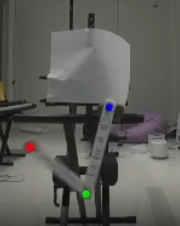
\includegraphics[width=0.9\textwidth]{02-pendulo-doble/DobleReal.png}
  \caption{Experimento del péndulo doble}
\end{figure}


En \autoref{fig:Trayectorias5} están las trayectorias del punto rojo del péndulo en cinco tiradas
desde la misma posición y con la misma velocidad inicial. Se puede
apreciar como al principio su trayectoria diverge muy rápidamente, pero
al final, cuando ya han perdido mucha velocidad, hacen todos un
recorrido muy similar hasta detenerse.


\begin{figure}[h]
  \centering
  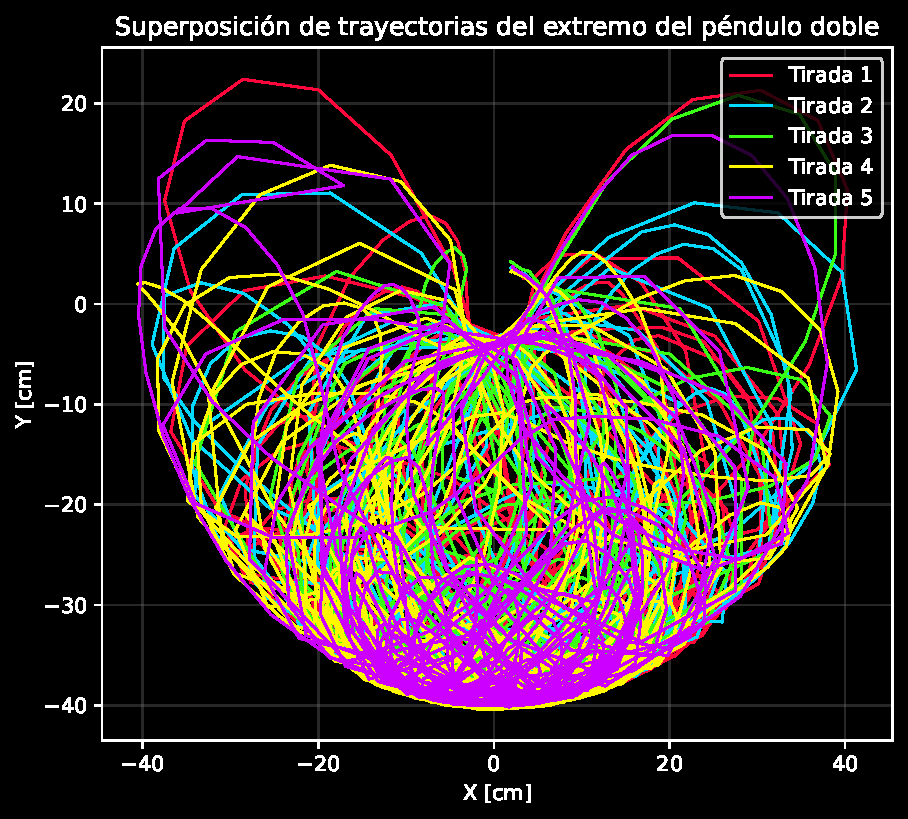
\includegraphics[width=0.9\textwidth]{02-pendulo-doble/experimentos_files/figure-pdf/cell-2-output-1.pdf}
  \caption{Trayectoria real de 5 tiradas de un péndulo doble}
  \label{fig:Trayectorias5}
\end{figure}

Esta es la animación que represente la trayectoria que han seguido tres
tiradas. El tiempo que aparece es el tiempo que ha pasado realmente, ya
que la trayectoria está ralentizada para que sea más fácil seguir como
van divergiendo.  \url{https://colacaos.github.io/ColaCAOS/02-pendulo-doble/trayectorias.gif}



\section{Comparación con el péndulo
simple}\label{comparaciuxf3n-con-el-puxe9ndulo-simple}

A continuación vamos a mostrar cinco tiradas del péndulo simple. El
péndulo es el mismo que en el caso anterior, lo único que fijamos el
pivote central para que no se mueva, por lo que pasamos de tener un
péndulo doble a uno simple. Igual que en el caso anterior, seguimos el
extremo con el punto rojo.

Como podemos ver en la siguiente figura, a pesar de lanzarse cada una de
las veces desde posiciones ligeramente distintas, las trayectorias son
idénticas.

\begin{figure}[h]
  \centering
  \includegraphics[width=0.9\textwidth]{02-pendulo-doble/experimentos_files/figure-pdf/cell-3-output-1.pdf}
  \caption{Trayectoria real de 5 tiradas de un péndulo doble}
\end{figure}

Y si miramos en la animación el ángulo del péndulo en cada una de las
trayectorias, vemos de nuevo que en función del tiempo las trayectorias
son muy similares \url{https://colacaos.github.io/ColaCAOS/02-pendulo-doble/theta_vs_time.gif}.

\begin{figure}[h]
  \centering
  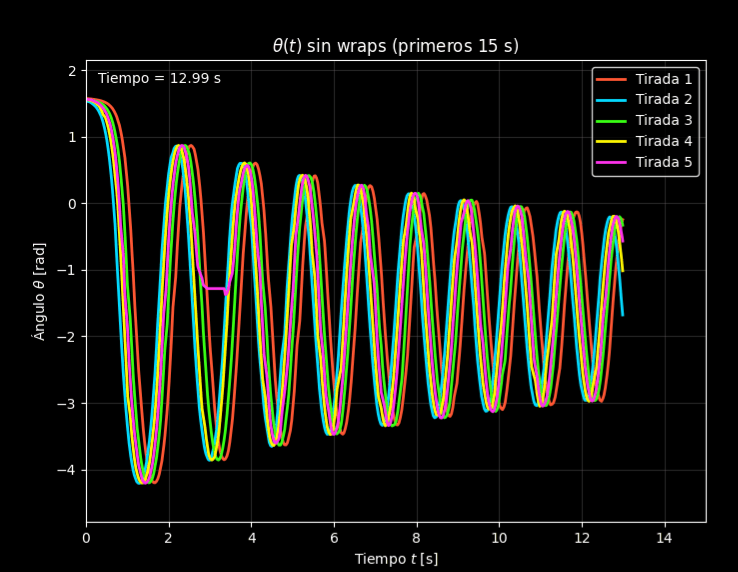
\includegraphics[width=0.99\textwidth]{02-pendulo-doble/theta_vs_time.png}
  \caption{Ángulos de 5 tiradas de un péndulo simple}
\end{figure}


Y si hacemos el ajuste de los tiempos iniciales el solape es casi total como se puede ver en la \autoref{fig:Solape}
\begin{figure}[h]
  \centering
  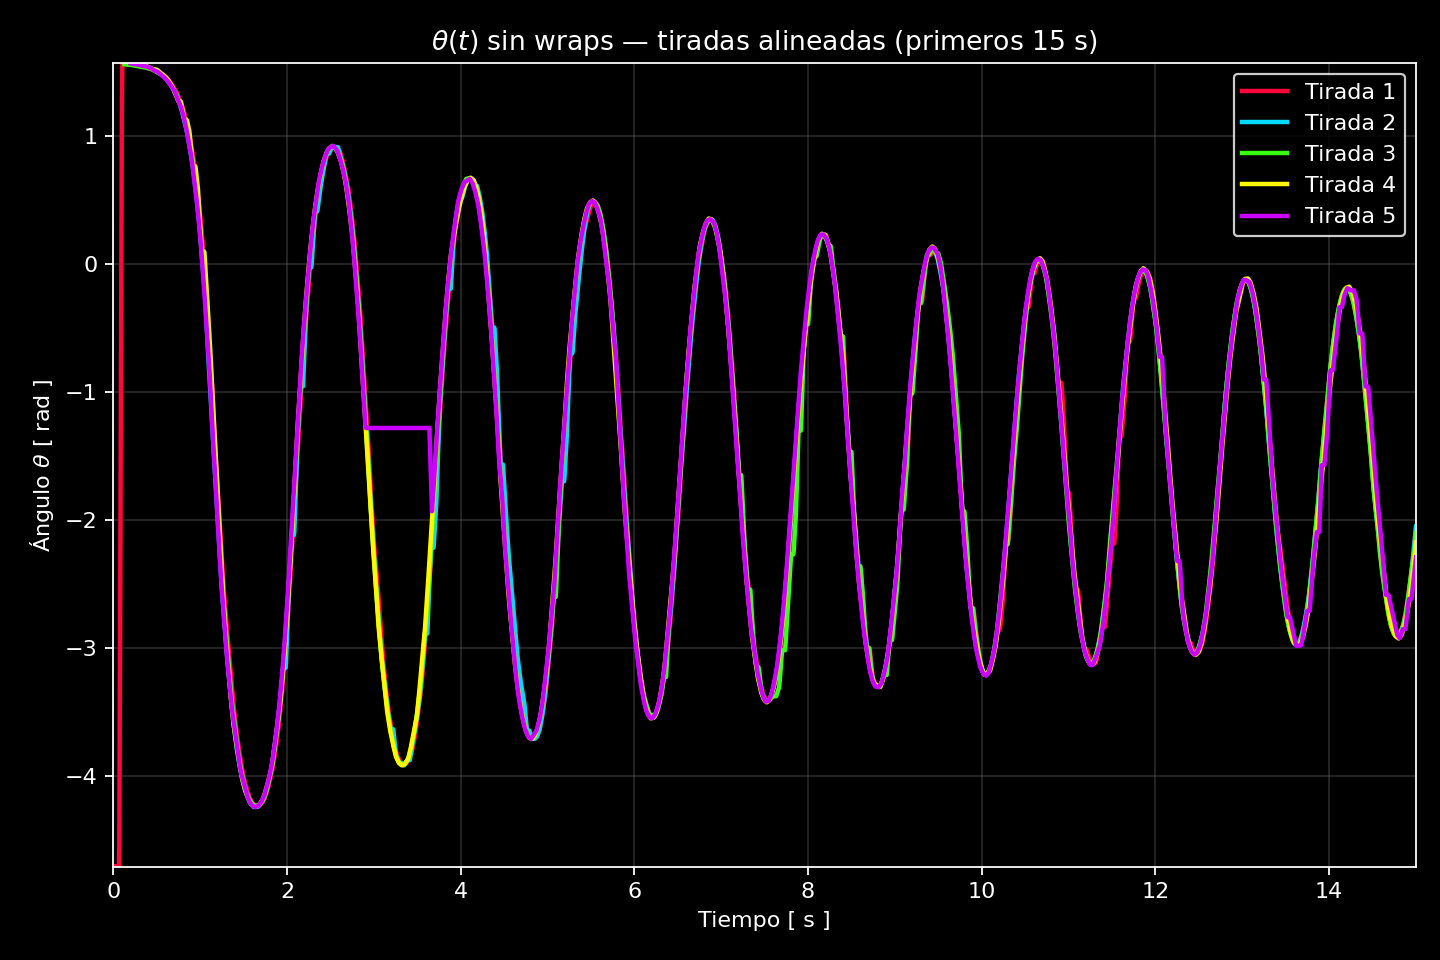
\includegraphics[width=0.99\textwidth]{02-pendulo-doble/theta_alineadas_sin_wraps.png}
  \caption{Ángulos de 5 tiradas de un péndulo simple ajustando el tiempo inicial}
  \label{fig:Solape}
\end{figure}



He hecho este mismo gráfico con los datos de las tiradas del péndulo
doble \url{https://colacaos.github.io/ColaCAOS/02-pendulo-doble/theta_vs_time_doble.gif}. El contraste con el péndulo doble es mayúsculo. En el péndulo
doble no había ni una sola trayectoria idéntica, divergían
continuamente. En el péndulo simple se ve como van iguales.

\begin{figure}[h]
  \centering
  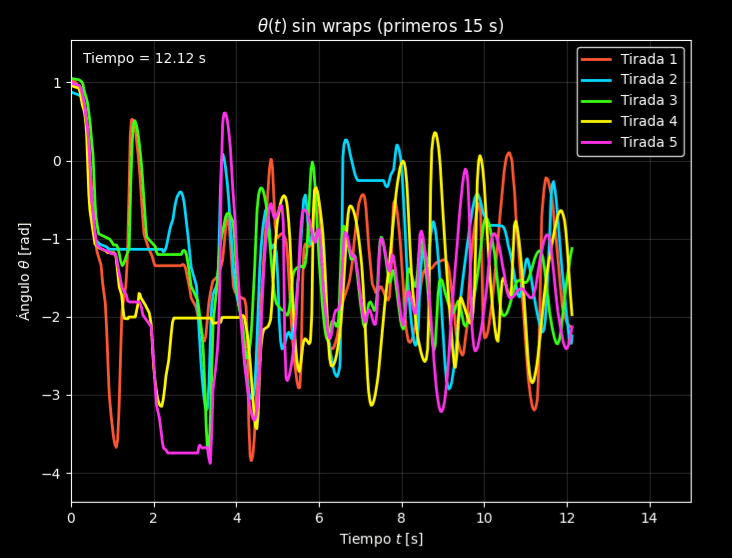
\includegraphics[width=0.99\textwidth]{02-pendulo-doble/theta_vs_time_doble.png}
  \caption{Ángulos de 5 tiradas de un péndulo doble}
\end{figure}


\part{La Meteorología y el Caos}

\chapter{Caos en las predicciones
meteorológicas}\label{caos-en-las-predicciones-meteoroluxf3gicas}

La meteorología es un ejemplo paradigmático de sistema caótico. Edward
Lorenz, en su famoso artículo de 1963 \url{https://journals.ametsoc.org/view/journals/atsc/20/2/1520-0469_1963_020_0130_dnf_2_0_co_2.xml}, demostró que pequeñas
perturbaciones en las condiciones iniciales pueden producir divergencias
exponenciales en la evolución del sistema atmosférico.
Esta propiedad se cuantifica mediante el \textbf{exponente de Lyapunov},
el cual mide la tasa a la que dos trayectorias inicialmente cercanas se
separan en el espacio de fases.

Como ya hemos mencionado uno de los retos del proyecto es demostrar que
el tiempo es un sistema caótico. En la versión digital de esta memoria en github está detallado el cálculo del exponente de Lyapunov cogiendo medidas reales de
variables como la temperatura y el viento, y analizándolas por medio de
rutinas hechas por ChatGPT (ver \url{https://colacaos.github.io/ColaCAOS/03-meteorologia/calculolyapunov.html}). Los valores resultantes son lo esperado: un
horizonte de predictibilidad de 10 días para la temperatura media
diaria.

Ahora vamos a emprender un método indirecto de cálculo desarrollado por mí. Las diferentes
organizaciones meteorológicas realizan todos los días predicciones de
hasta 14 días. Puesto que el tiempo es caótico, este caos se tiene que
reflejar en el error de las predicciones. A medida que aumenta la
distancia con respecto al día actual, el error tiene que aumentar. Este
incremento no será lineal sino que será exponencial, de acuerdo a la
teoría que ya hemos visto. Si cogemos los errores, y hacemos un
logaritmo, podremos hacer una regresión lineal del logaritmo del error,
lo que nos dará el exponente de Lyapunov. Así de sencillo. Se trata de
una medida indirecta, pero creo que muy sencilla del exponente de
Lyapunov. El punto fundamental es asumir que los modelos implementados en los supercomputadores de las agencias meteorológicas son fidedignos a la realidad, y que el error en los pronósticos se debe a los errores de las condiciones iniciales. De esta manera podemos ver como las perturbaciones iniciales se propagan en el tiempo. 

\section{Proceso de Recopilación de Datos Mediante el Script de
Python}\label{proceso-de-recopilaciuxf3n-de-datos-mediante-el-script-de-python}

En este punto lo primero que tenemos que hacer es recopilar datos. En
este caso en vez de usar open-meteo, usé Visual Crossing
(https://www.visualcrossing.com/) , que dispone también de una utilidad
gratuita para descargar previsiones meteorológicas. Para ello, pedí a
ChatGPT que hiciera un script para coger los datos de Visual Crossing.
El script desarrollado tiene dos funciones principales, diseñadas para
ir acumulando la información necesaria a lo largo del tiempo:

\emph{a) Registro de Pronósticos (``Forecast'')}

Cada día se obtiene un pronóstico para 15 días (el día actual + 14 días
de anticipación) a través de la API de Visual Crossing. Para cada
parámetro (temperatura, humedad, presión y velocidad del viento), se
crea un archivo CSV en el que cada fila contiene:

\begin{itemize}
\tightlist
\item
  \textbf{Columna 1:} La fecha de creación del pronóstico (formato
  americano: M-D-YYYY).
\item
  \textbf{Columnas 2 a 15:} Los valores predichos para 1 día adelante, 2
  días adelante, \ldots, hasta 14 días adelante.
\end{itemize}

Matemáticamente, si denotamos por \(F_{\text{param}}(d, n)\) el valor
predicho para el parámetro en el día \(d+n\) cuando el pronóstico se
realizó en el día \(d\), la fila correspondiente al pronóstico realizado
en la fecha \(d\) es:

\begin{equation}
\text{Fila}_d = \bigl[ d,\; F_{\text{param}}(d,1),\; F_{\text{param}}(d,2),\; \dots,\; F_{\text{param}}(d,14) \bigr]
\end{equation}

\emph{b) Registro Retroactivo (``Retro'')}

El propósito de este archivo es reconstruir, para cada día objetivo, la
evolución de los pronósticos hechos en días anteriores y compararlos con
el valor observado real. Para cada parámetro se crea un archivo CSV en
el que cada fila contiene:

\begin{itemize}
\tightlist
\item
  \textbf{Columna 1:} La fecha del día objetivo (por ejemplo, ayer,
  formato M-D-YYYY).
\item
  \textbf{Columna 2:} El valor observado históricamente para ese día.
\item
  \textbf{Columnas 3 a 16:} Los pronósticos para ese mismo día,
  realizados desde 1 hasta 14 días antes.
\end{itemize}

En otras palabras, para un día objetivo \(d_{\text{target}}\), se
recupera el pronóstico realizado en \(d_{\text{target}} - n\) (para
\(n = 1,2,\dots,14\)) y se toma el valor predicho correspondiente al
\(n\)-ésimo día. La fila retroactiva es:

\begin{equation}
\text{Retro}_d = \bigl[ d_{\text{target}},\; O(d_{\text{target}}),\; F_{\text{param}}(d_{\text{target}}-1,1),\; F_{\text{param}}(d_{\text{target}}-2,2),\; \dots,\; F_{\text{param}}(d_{\text{target}}-14,14) \bigr]
\end{equation}

donde \(O(d_{\text{target}})\) es el valor observado real para el
parámetro en el día objetivo.

La estructura de los dos ficheros se detalla en la siguiente figura


\begin{figure}[h]
  \centering
  \scalebox{1.5}{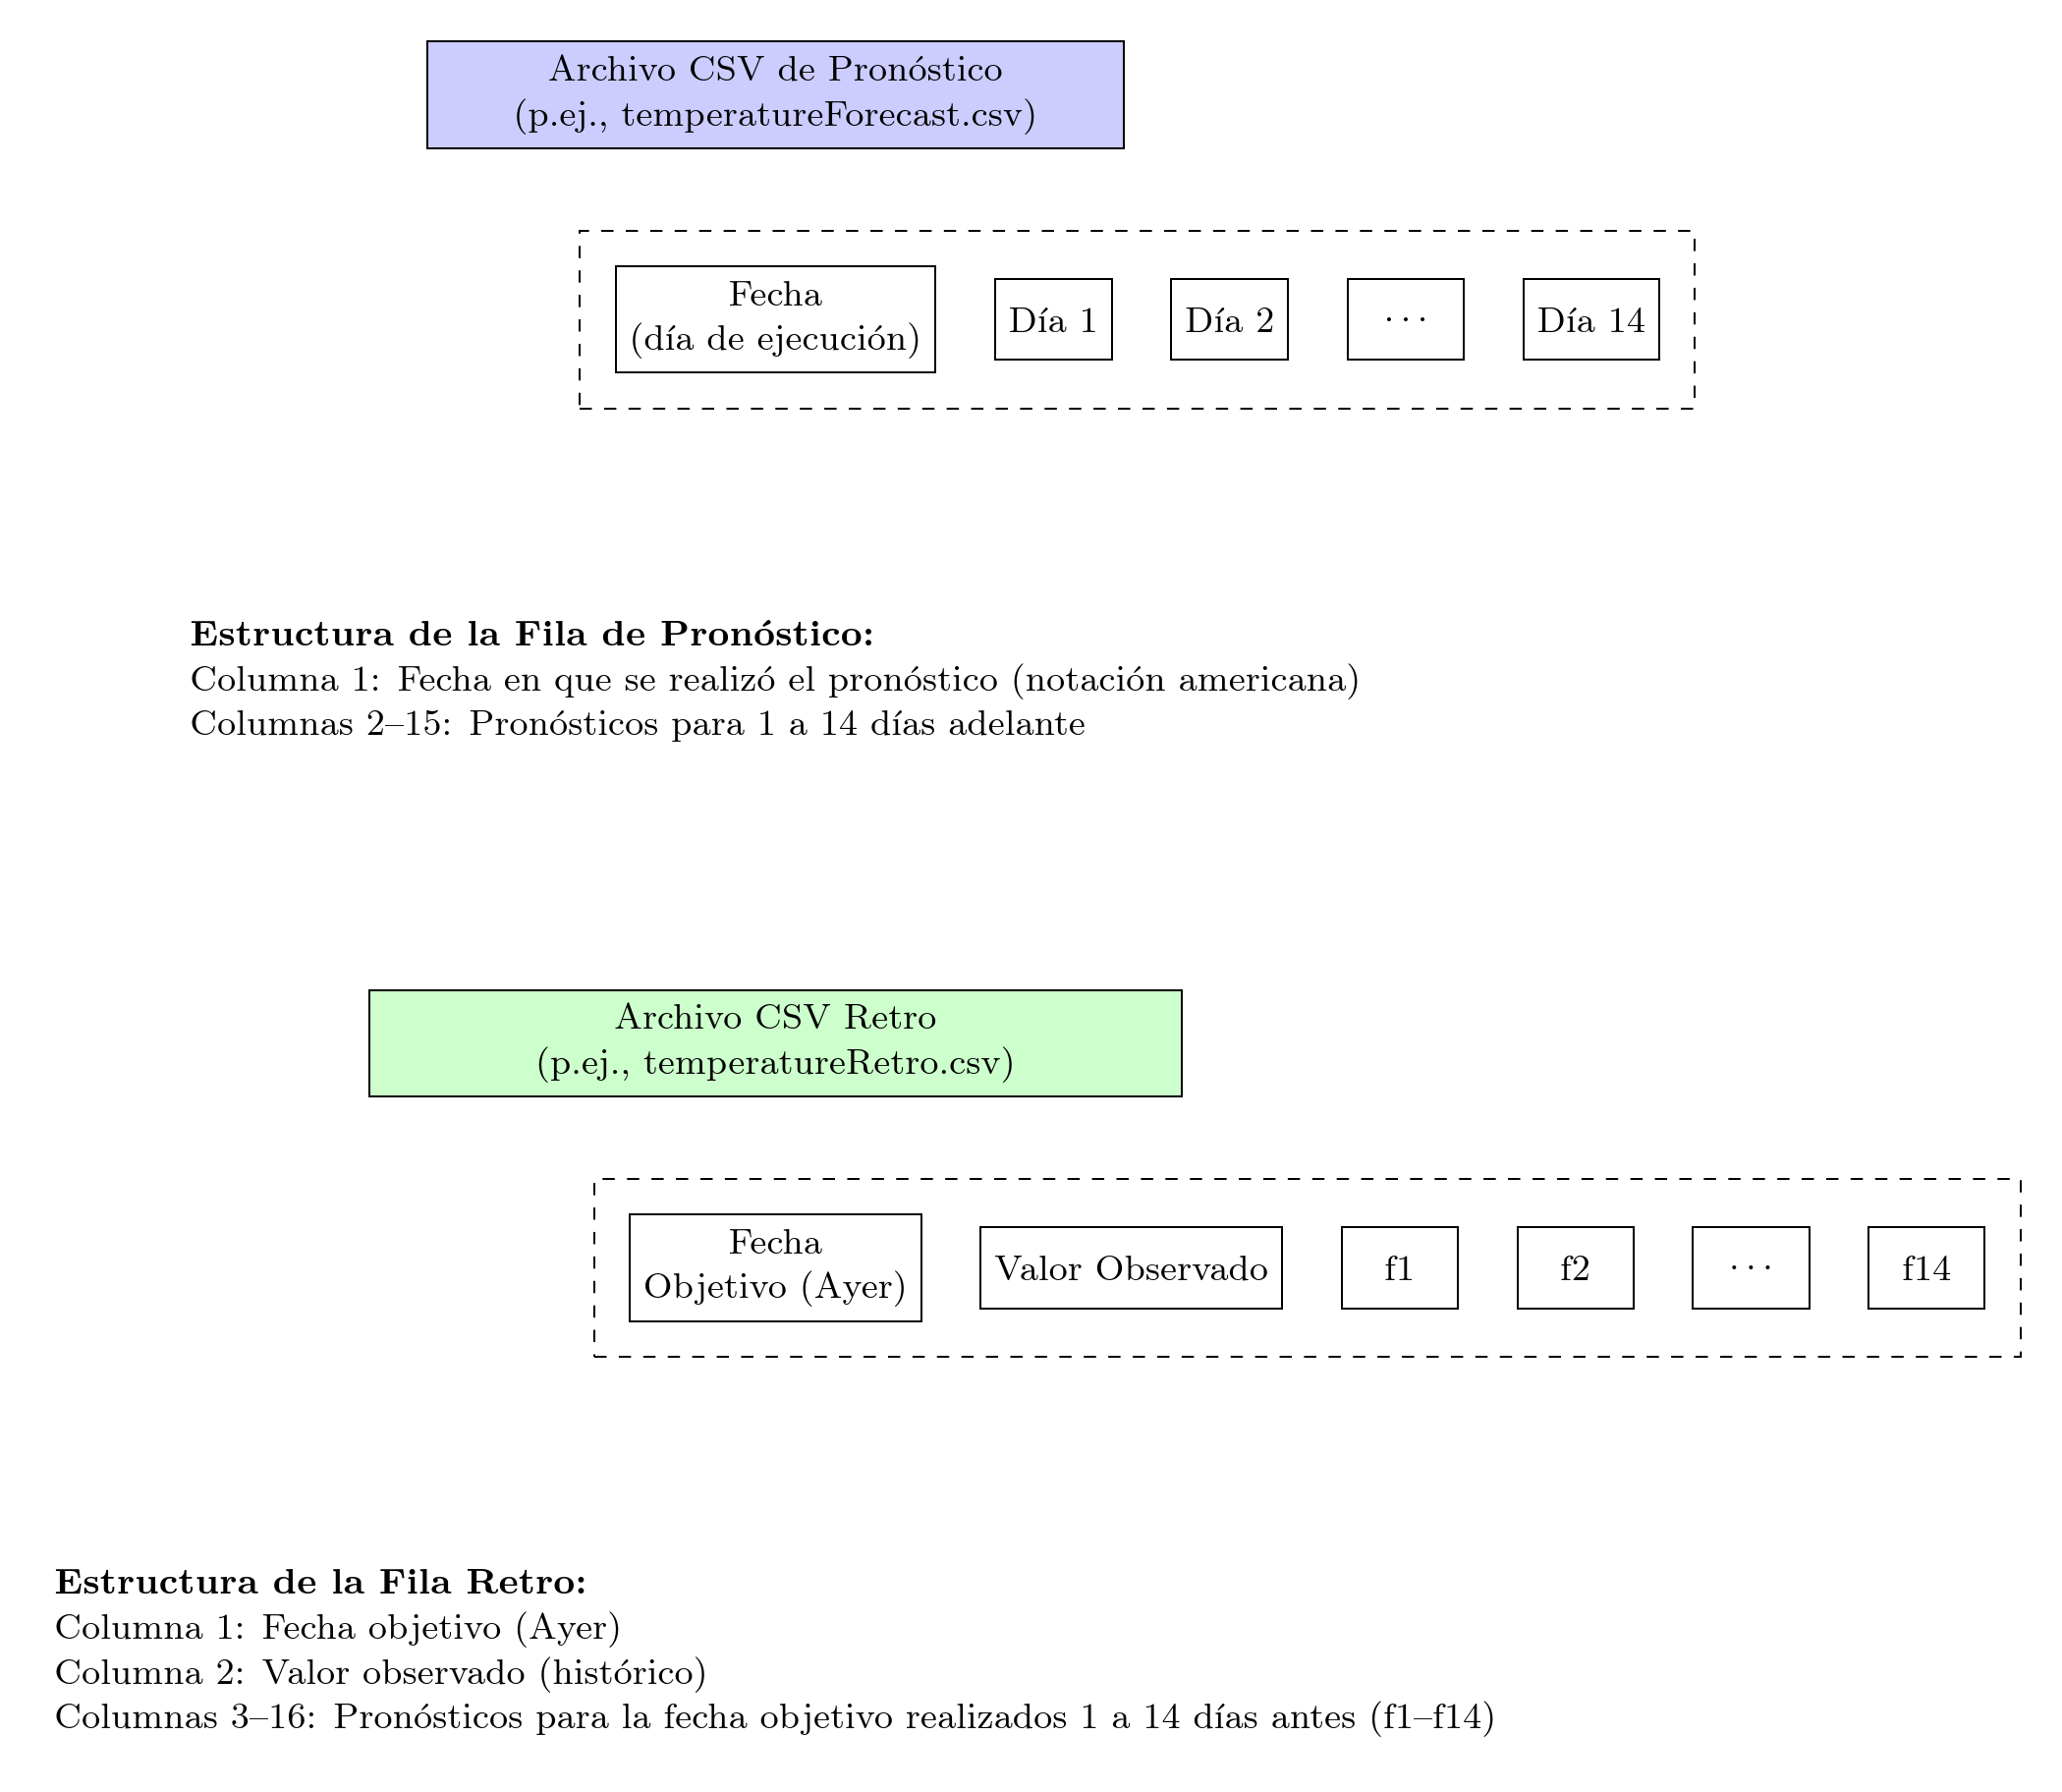
\includegraphics{03-meteorologia/FicheroCSV.png}}
  \caption{Estructura de los ficheros de observaciones y pronósticos}
\end{figure}

Y el procedimiento que hace el script diariamente se detalla a
continuación.

\begin{figure}[h]
  \centering
  \scalebox{1.5}{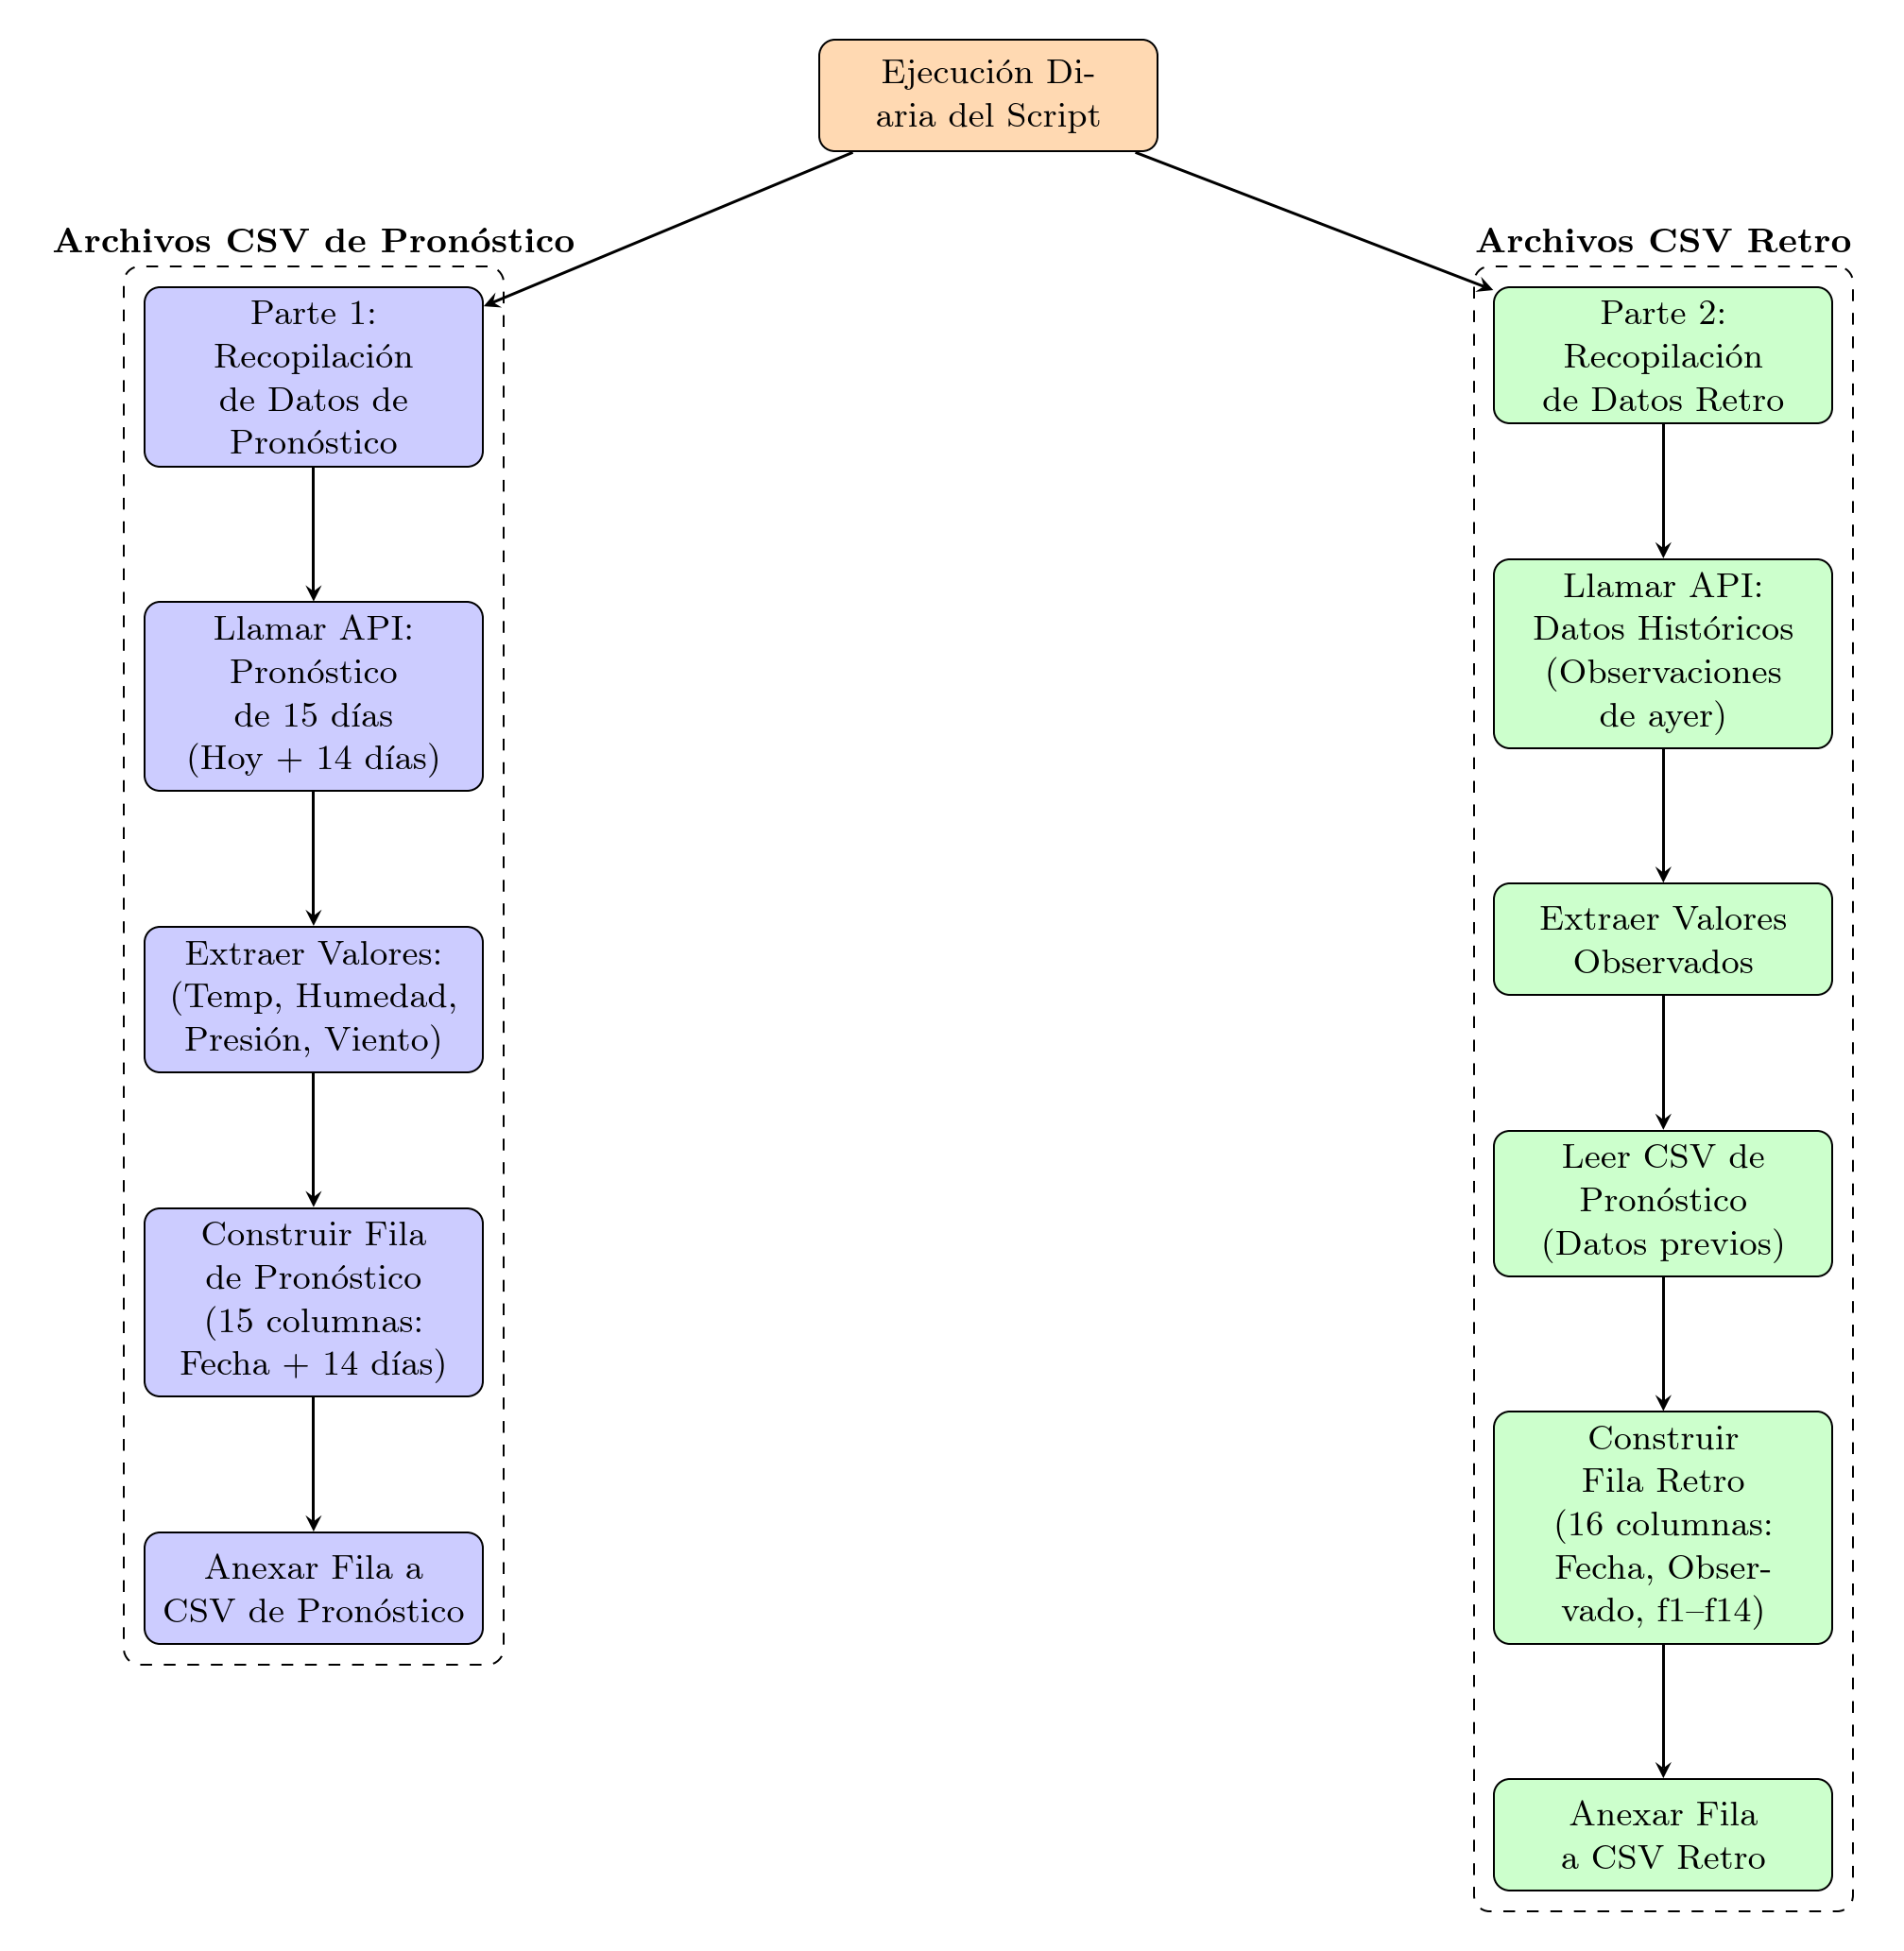
\includegraphics{03-meteorologia/EjecucionDiaria.png}}
  \caption{Estructura de los ficheros de observaciones y pronósticos}
\end{figure}


El error de cada pronóstico se define como:

\begin{equation}
e(n) = \bigl| F_{\text{param}}(d_{\text{target}}-n, n) - O(d_{\text{target}}) \bigr|
\end{equation}

para \(n = 1,2,\dots,14\). Esta serie \(\{e(n)\}\) representa cómo varía
el error en función del tiempo de anticipación.

\section{Análisis de Datos y Determinación del Coeficiente de
Lyapunov}\label{anuxe1lisis-de-datos-y-determinaciuxf3n-del-coeficiente-de-lyapunov}

\emph{a) Enfoque Teórico Clásico}

En un sistema caótico, la separación entre dos trayectorias evoluciona
de forma exponencial. Asumiendo que el error en el pronóstico \(e(n)\)
crece de manera similar, se modela como:

\begin{equation}
e(n) = e(0)\, e^{\lambda n}
\end{equation}

Tomando logaritmos:

\begin{equation}
\ln e(n) = \ln e(0) + \lambda n
\end{equation}

Por lo tanto, si se realiza un ajuste lineal de \(\ln e(n)\) en función
de \(n\), la pendiente de la recta brinda una estimación empírica de
\(\lambda\).

\emph{b) Enfoque Empírico Propuesto}

En este estudio, en lugar de disponer de dos trayectorias
infinitesimalmente separadas, se utilizan las diferencias en las
predicciones realizadas en distintos días para el mismo objetivo. Cada
error \(e(n)\) se obtiene como la diferencia entre el pronóstico hecho
\(n\) días antes y el valor observado:

\begin{equation}
e(n) = \bigl| F_{\text{param}}(d_{\text{target}}-n, n) - O(d_{\text{target}}) \bigr|
\end{equation}

La estimación empírica del exponente de Lyapunov se obtiene realizando
un ajuste lineal de:

\begin{equation}
\ln e(n) = \ln e(0) + \lambda_{\text{emp}} n
\end{equation}

donde \(\lambda_{\text{emp}}\) es la pendiente obtenida a partir de la
regresión lineal sobre los datos \((n, \ln e(n))\).

Esto ya lo vimos en la sección \hyperref[sec-sensibilidad]{Efecto
mariposa}. En esa sección vimos como el error iba creciendo
exponencialemnte, y al hacer el logaritmo nos quedó una recta cuya
pendiente era el exponente de Lyapunov de la función logística para ese
valor de \(r\). En este caso, veremos que el error de pronóstico crece
también exponencialmente, no linealmente, lo que al hacer el logaritmo
nos permitirá sacar la pendiente y por tanto el exponente de Lyapunov.

\emph{c) Confrontación con la Fórmula Tradicional}

\textbf{Fórmula Tradicional:}

\begin{equation}
\lambda = \lim_{t \to \infty} \frac{1}{t} \ln \frac{|\delta x(t)|}{|\delta x(0)|}
\end{equation}

\textbf{Fórmula Empírica del Estudio:}

\begin{equation}
\lambda_{\text{emp}} \approx \text{slope}\bigl(\ln e(n)\ \text{vs.}\ n\bigr)
\end{equation}

En este caso, \(e(n)\) incorpora tanto la sensibilidad a las condiciones
iniciales como los errores inherentes del modelo de pronóstico. Además,
el análisis se realiza sobre un rango discreto de días (1 a 14), por lo
que \(\lambda_{\text{emp}}\) debe interpretarse como una aproximación de
la tasa de divergencia del error.

\section{Resultados}\label{resultados-2}

Durante los meses de febrero, marzo y abril estuve recopilando las
predicciones y los valores observados de temperatura, humedad, viento y
presión atmosférica para Galapagar.

El conjunto de errores para cada día de la predicción se muestran a
continuación (cada línea representa un día en el que se realiza la
predicción).

\begin{figure}[h]
  \centering
  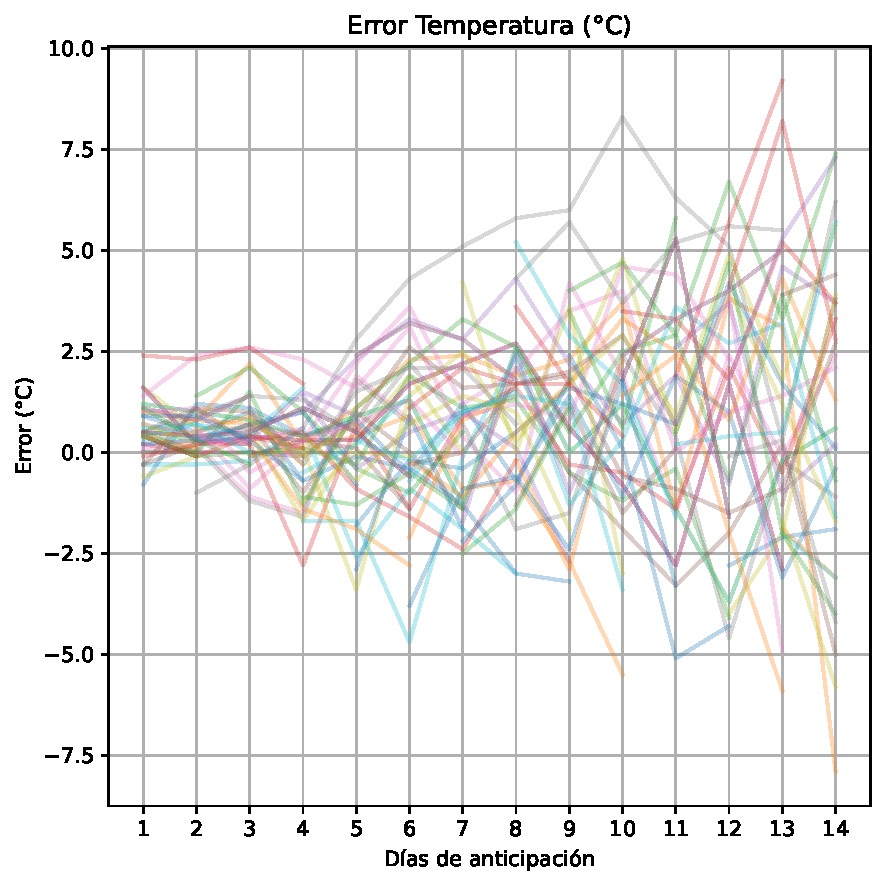
\includegraphics[width=0.99\textwidth]{03-meteorologia/predicciones_files/figure-pdf/cell-2-output-1.pdf}
  \caption{Error de temperatura en escala lineal}
\end{figure}

\begin{figure}[h]
  \centering
  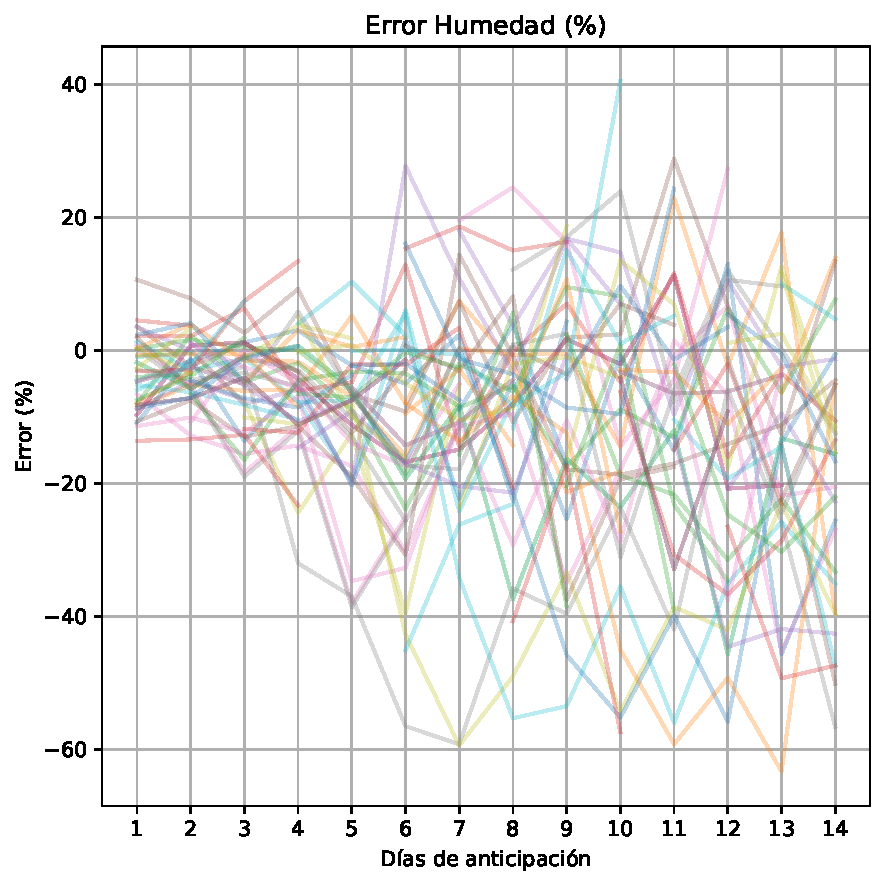
\includegraphics[width=0.99\textwidth]{03-meteorologia/predicciones_files/figure-pdf/cell-2-output-2.pdf}
  \caption{Error de humedad en escala lineal}
\end{figure}

\begin{figure}[h]
  \centering
  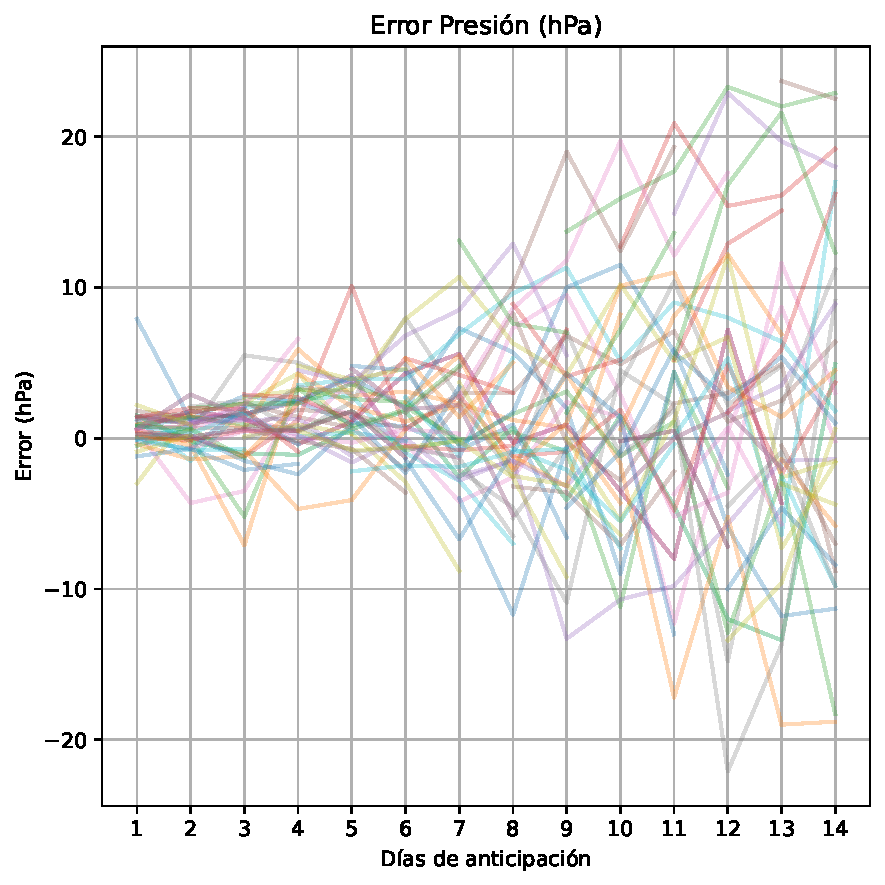
\includegraphics[width=0.99\textwidth]{03-meteorologia/predicciones_files/figure-pdf/cell-2-output-3.pdf}
  \caption{Error de presión en escala lineal}
\end{figure}

\begin{figure}[h]
  \centering
  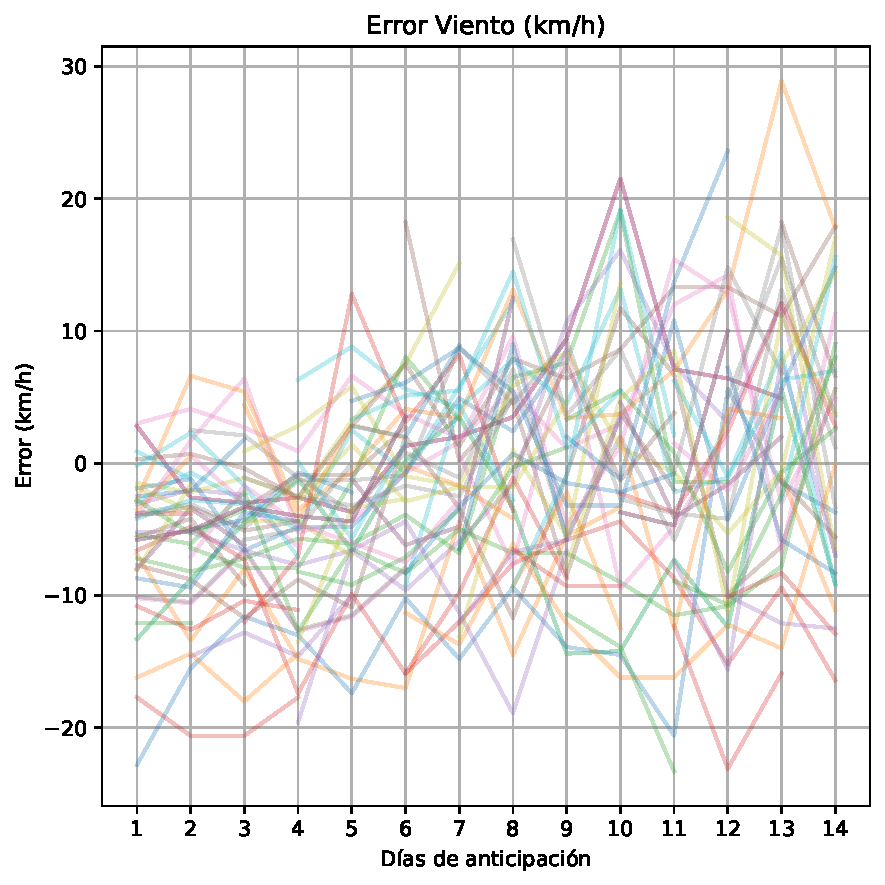
\includegraphics[width=0.99\textwidth]{03-meteorologia/predicciones_files/figure-pdf/cell-2-output-4.pdf}
  \caption{Error de velocidad del viento en escala lineal}
\end{figure}

Los errores medios en valor absoluto de predicción en función del número
de días anteriores en los que se hizo la predicción se muestran a
continuación. Se ve claramente que los errores van aumentando
exponencialmente.

\begin{figure}[h]
  \centering
  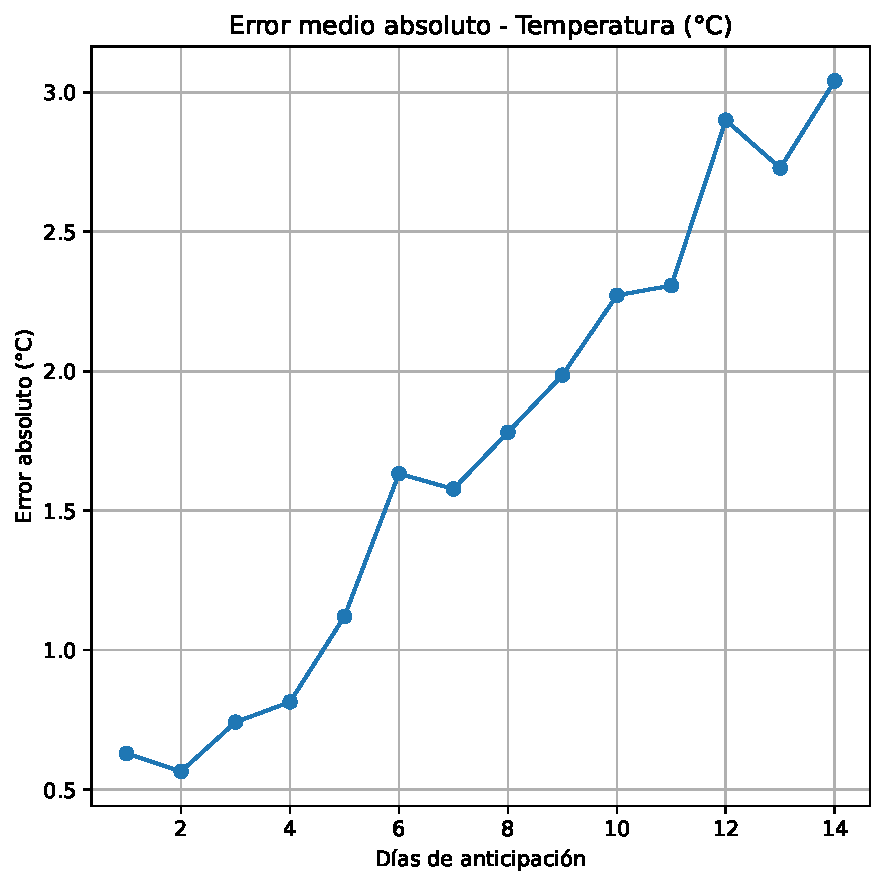
\includegraphics[width=0.99\textwidth]{03-meteorologia/predicciones_files/figure-pdf/cell-3-output-1.pdf}
  \caption{Error medio absoluto de temperatura en escala lineal}
\end{figure}

\begin{figure}[h]
  \centering
  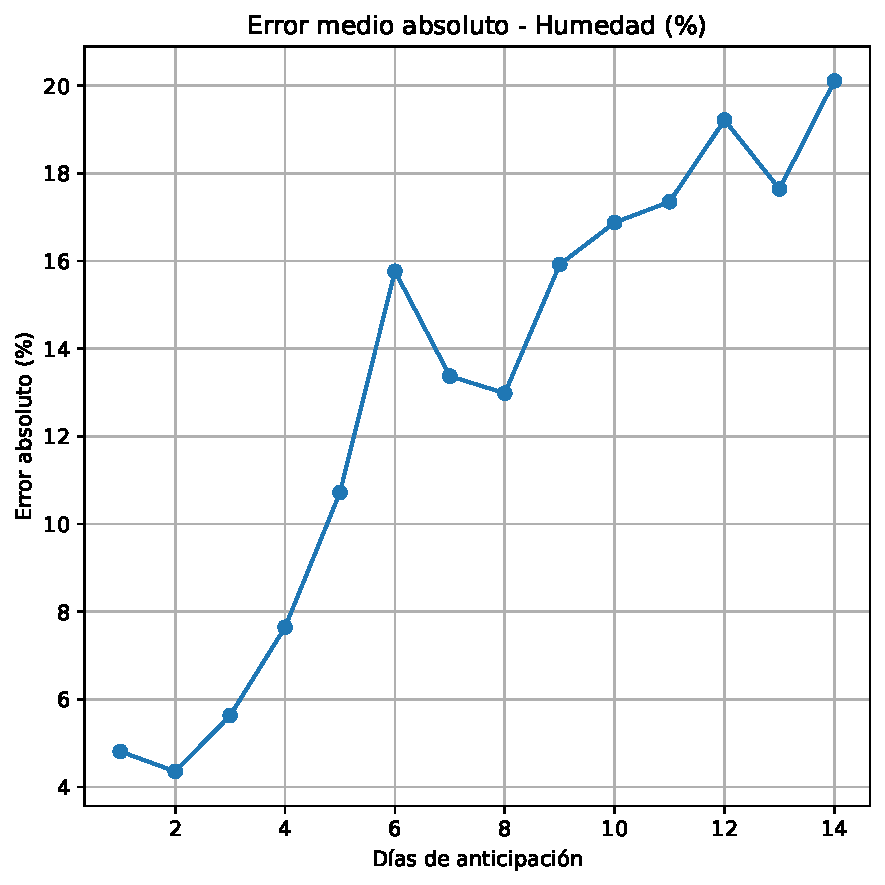
\includegraphics[width=0.99\textwidth]{03-meteorologia/predicciones_files/figure-pdf/cell-3-output-2.pdf}
  \caption{Error medio absoluto de humedad en escala lineal}
\end{figure}

\begin{figure}[h]
  \centering
  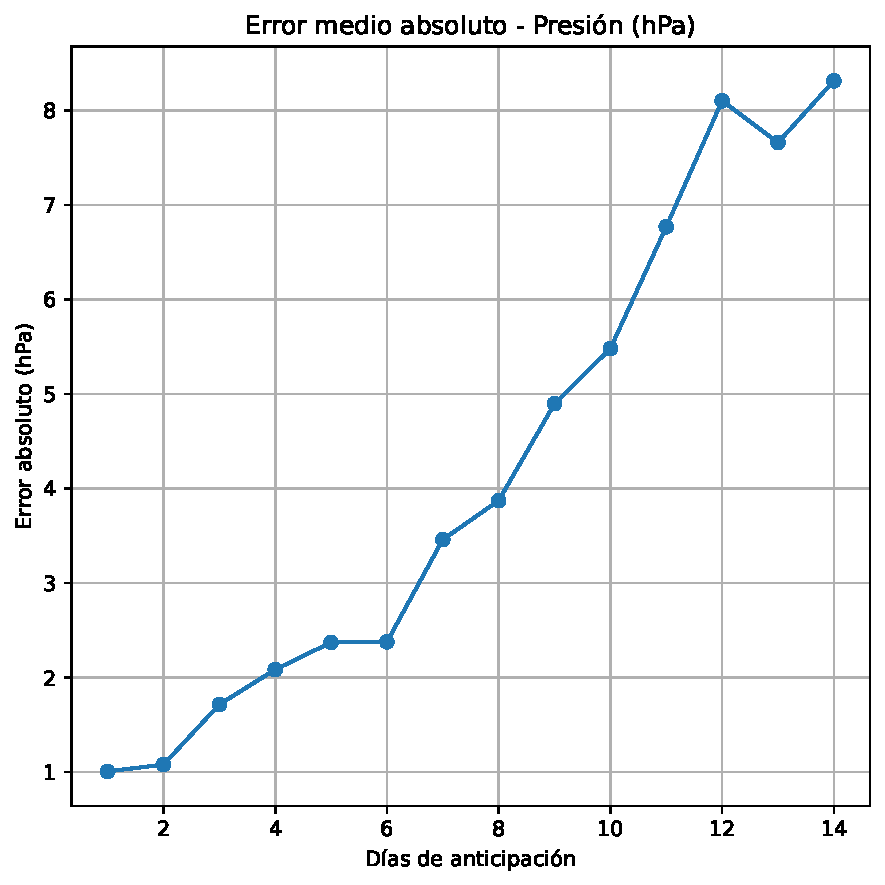
\includegraphics[width=0.99\textwidth]{03-meteorologia/predicciones_files/figure-pdf/cell-3-output-3.pdf}
  \caption{Error medio absoluto de presión en escala lineal}
\end{figure}

\begin{figure}[h]
  \centering
  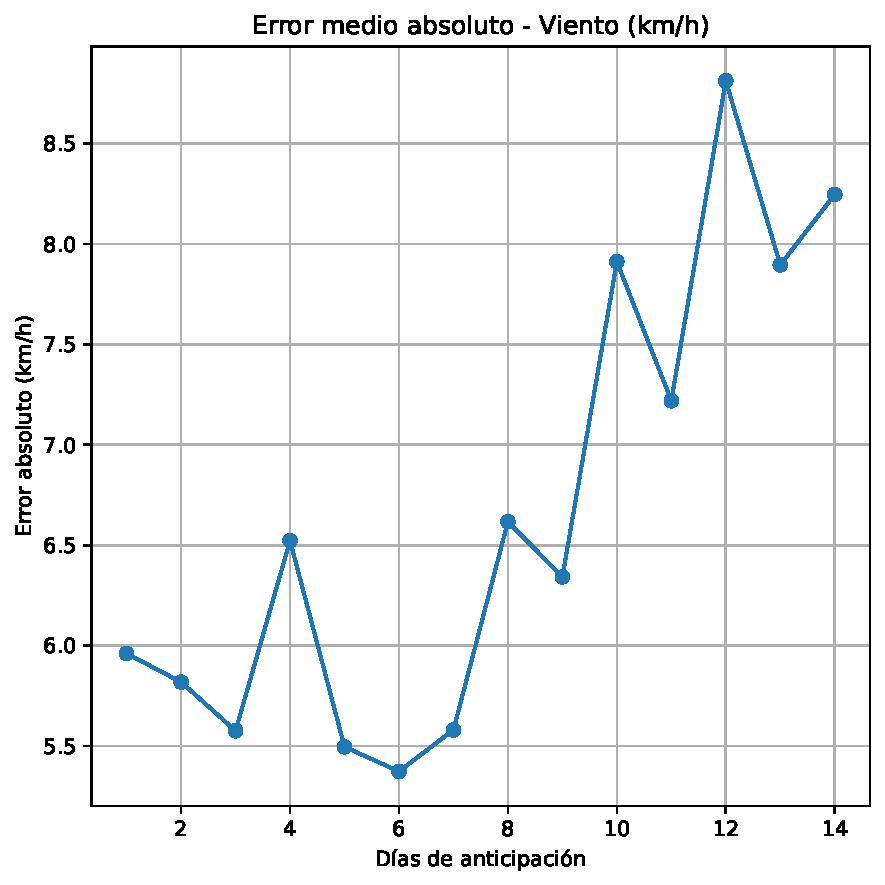
\includegraphics[width=0.99\textwidth]{03-meteorologia/predicciones_files/figure-pdf/cell-3-output-4.pdf}
  \caption{Error medio absoluto de velocidad del viento en escala lineal}
\end{figure}


Y ahora le pedimos a ChatGPT que nos calcule el exponente de Lyapunov, y
que nos trace de forma superpuesta el error de acuerdo al exponente de
Lyapunov.


\begin{figure}[h]
  \centering
  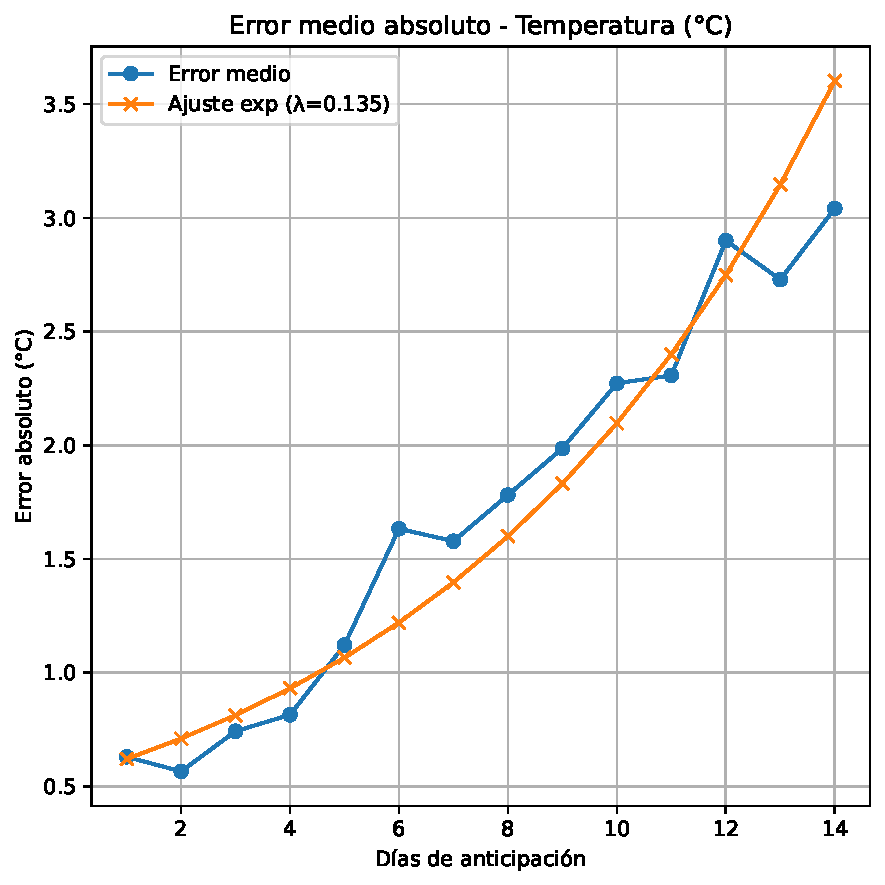
\includegraphics[width=0.99\textwidth]{03-meteorologia/predicciones_files/figure-pdf/cell-4-output-1.pdf}
  \caption{Error medio absoluto de temperatura y ajuste de regresión}
\end{figure}

\begin{figure}[h]
  \centering
  \includegraphics[width=0.99\textwidth]{03-meteorologia/predicciones_files/figure-pdf/cell-4-output-2.pdf}
  \caption{Error medio absoluto de humedad y ajuste de regresión}
\end{figure}

\begin{figure}[h]
  \centering
  \includegraphics[width=0.99\textwidth]{03-meteorologia/predicciones_files/figure-pdf/cell-4-output-3.pdf}
  \caption{Error medio absoluto de presión y ajuste de regresión}
\end{figure}

\begin{figure}[h]
  \centering
  \includegraphics[width=0.99\textwidth]{03-meteorologia/predicciones_files/figure-pdf/cell-4-output-4.pdf}
  \caption{Error medio absoluto de velocidad del viento y ajuste de regresión}
\end{figure}

Los exponentes de Lyapunov salen más pequeños que los calculados
mediante las series históricas en la sección anterior
\hyperref[sec-lyapunov]{Predictibilidad}. Hay que tener en cuenta que
los exponentes en la sección anterior se tomaban sobre la base de 75
años, mientras que aquí tenemos un experimento más limitado, solamente
tres meses, por lo que es normal que no cuadren del todo los datos. Sin
embargo, tal y como hipotizamos, estamos alrededor de las dos semanas
como límite de predictibilidad.

Además, lo que es muy relevante, es ver como el error de predicción
crece exponencialmente. Se ponen de manifiesto dos causas: la
inexactitud de las condiciones iniciales, y la inexactitud de los
modelos y sus cómputos. Puesto que el sistema modelado es caótico, tal y
como esperábamos los errores crecen exponencialmente.


\chapter{Entrevista con expertos de la
AEMET}\label{entrevista-con-expertos-de-la-aemet}

El Jueves 19 de Junio tuve la oportunidad de tener una entrevista con
dos meteorólogos de la Agencia Estatal de Meteorología para hacerles
algunas preguntas sobre la parte del proyecto donde se estudia el caos
en la predicción meteorológica y climática. De esta manera he podido
incluir también la opinión de expertos en el tema en este proyecto. Aquí
están todas las preguntas que hice durante la entrevista y cuáles fueron
las respuestas de los expertos:

\section{¿Qué condiciones atmosféricas hacen que el sistema sea más
caótico y por tanto que sea más difícil llevar a cabo una predicción
meteorológica fiable, y cuales lo hacen más
fácil?}\label{quuxe9-condiciones-atmosfuxe9ricas-hacen-que-el-sistema-sea-muxe1s-cauxf3tico-y-por-tanto-que-sea-muxe1s-difuxedcil-llevar-a-cabo-una-predicciuxf3n-meteoroluxf3gica-fiable-y-cuales-lo-hacen-muxe1s-fuxe1cil}

Las condiciones en las que la atmósfera es más inestable como borrascas
o ambientes de tormenta, porque es más difícil establecer unas
condiciones iniciales que no tengan mucho error y que sean precisas.
Esto hace que el error inicial en las mediciones sea grande y que se
propague más rápidamente.

\section{¿Existe un horizonte de predictibilidad a partir del cual las
predicciones meteorológicas no van a llegar a ser fiables nunca sin
importar los avances tecnológicos y en los modelos que se puedan llevar
a cabo en el futuro? ¿Cuál consideráis que es el horizonte de
predictibilidad
actualmente?}\label{existe-un-horizonte-de-predictibilidad-a-partir-del-cual-las-predicciones-meteoroluxf3gicas-no-van-a-llegar-a-ser-fiables-nunca-sin-importar-los-avances-tecnoluxf3gicos-y-en-los-modelos-que-se-puedan-llevar-a-cabo-en-el-futuro-cuuxe1l-consideruxe1is-que-es-el-horizonte-de-predictibilidad-actualmente}

Sí, existe un horizonte de predictibilidad en meteorología, y es teórico
y práctico al mismo tiempo. Se trata de un límite físico-matemático
impuesto por la naturaleza del sistema atmosférico: un sistema caótico y
no lineal. Este límite está alrededor de los 20 días y no importa cuán
potentes sean los ordenadores del futuro o lo precisos que sean los
sensores, este límite no va a poder superarse.

\section{¿Qué avances tecnológicos o metodológicos han mejorado más la
capacidad predictiva frente a la naturaleza caótica de la
atmósfera?}\label{quuxe9-avances-tecnoluxf3gicos-o-metodoluxf3gicos-han-mejorado-muxe1s-la-capacidad-predictiva-frente-a-la-naturaleza-cauxf3tica-de-la-atmuxf3sfera}

Los satélites, ya que permiten tomar mediciones de las diferentes capas
de la atmósfera con más facilidad y de zonas más amplias que los globos
meteorológicos, la capacidad computacional de los superordenadores y que
se van añadiendo nuevos términos a las ecuaciones que dan más detalle y
ayudan a mejorarlas.

\section{¿Existe algún parámetro como precipitación, viento, temperatura
o humedad que sea más difícil de predecir y más caótico que otro o por
el contrario más fácil de predecir que
otro?}\label{existe-alguxfan-paruxe1metro-como-precipitaciuxf3n-viento-temperatura-o-humedad-que-sea-muxe1s-difuxedcil-de-predecir-y-muxe1s-cauxf3tico-que-otro-o-por-el-contrario-muxe1s-fuxe1cil-de-predecir-que-otro}

Si, los parámetros que son derivados de los demás que se obtienen
sabiendo otros como la precipitación o la nubosidad, ya que no salen
directamente de las ecuaciones que se utilizan en las predicciones, si
no que se obtienen teniendo en cuenta mucho parámetros más simples que
si salen de las ecuaciones

\section{¿Cómo se tiene en cuenta el error que existe a la hora de hacer
las simulaciones de la atmósfera, que vienen dados por el propio límite
de los ordenadores en cuanto a precisión en los
decimales?}\label{cuxf3mo-se-tiene-en-cuenta-el-error-que-existe-a-la-hora-de-hacer-las-simulaciones-de-la-atmuxf3sfera-que-vienen-dados-por-el-propio-luxedmite-de-los-ordenadores-en-cuanto-a-precisiuxf3n-en-los-decimales}

No existe ningún método como tal para reducir o eliminar ese error pero
muchas veces no se llega a aprovechar toda la precisión que te permite
el ordenador ya que los cálculos llevan mucho tiempo, y muchas veces se
necesitan tener terminadas las predicciones rápidamente.

\section{¿Existe sensibilidad a las condiciones iniciales en las
predicciones climáticas a largo plazo de la misma manera que en la
predicción meteorológica, donde acaban dando lugar al
caos?}\label{existe-sensibilidad-a-las-condiciones-iniciales-en-las-predicciones-climuxe1ticas-a-largo-plazo-de-la-misma-manera-que-en-la-predicciuxf3n-meteoroluxf3gica-donde-acaban-dando-lugar-al-caos}

Si existe pero las condiciones iniciales afectan menos ya que las
ecuaciones utilizadas se simplifican y se vuelven lineales. Por otra
parte el resultado no tiene que ser tan preciso ya que lo que se obtiene
es una media. Sin embargo, aunque no sea casi caótico sigue siendo
difícil establecer las condiciones iniciales por lo que el error inicial
puede acabar propagándose aunque más lentamente que en las predicciones
meteorológicas.

\section{¿Existe alguna condición o tipo de clima el cual presenta más o
menos caos a la hora de realizar predicciones a largo
plazo?}\label{existe-alguna-condiciuxf3n-o-tipo-de-clima-el-cual-presenta-muxe1s-o-menos-caos-a-la-hora-de-realizar-predicciones-a-largo-plazo}

Sí que existen algunos climas que son más predecibles que otros a largo
plazo. En predicción climática, el caos no desaparece, pero su impacto
depende mucho del contexto:Si una región está controlada por
forzamientos globales regulares, como El Niño, es menos caótica y más
predecible. Si depende del ruido interno de la atmósfera o de factores
locales, el caos reina y la predictibilidad climática estacional es
baja.

\section{¿Es el caos la razón de que algunas de las predicciones
climatológicas hechas hace varias décadas no hayan sido muy precisas o
incluso algunas hayan llegado a
fallar?}\label{es-el-caos-la-razuxf3n-de-que-algunas-de-las-predicciones-climatoluxf3gicas-hechas-hace-varias-duxe9cadas-no-hayan-sido-muy-precisas-o-incluso-algunas-hayan-llegado-a-fallar}

Sí puede serlo algunas veces, aunque también influyen muchos factores
externos como la actividad humana que no se pueden predecir.

\part{El Clima y el Caos}

\chapter{Clima}\label{clima}

Llegamos a la parte más cualitativa y menos cuantitativa del proyecto,
no por ello menos importante. Como bien se manifiesta en los medios de
comunicación y en la comunidad científica la predicción del clima es uno
los puntos más importantes para la Humanidad. Si bien en el capítulo
anterior hemos investigado sobre como afecta el caos a la previsión
meteorológica ahora vamos a hacer lo mismo con el clima.

Con el tiempo meteorológico a corto plazo todo el mundo asume que las
previsiones meteorológicas dejan de tener validez a los diez días. En
este proyecto hemos visto que esto se debe a que la atmósfera es un
sistema caótico, muy sensible, por lo tanto, a las condiciones
iniciales.

Con el clima curiosamente, la sensación general que hay en la sociedad
es que puede predecirse. Cada ciertos años el IPCC nos da sus
proyecciones sobre el clima para los próximos 100 años, y lo tomamos
como válido dado el gran consenso científico en torno a estas
proyecciones. ¿Cómo puede ser ésto?. No podemos predecir el tiempo a
diez días, pero sí a cien años. A continuación, durante este capítulo,
veremos los matices que hay detrás de todo esto.

\section{Clima y Caos. Historia}\label{clima-y-caos.-historia}

Empezaremos por ver cuál es la postura oficial del IPCC sobre la
predictibilidad del clima. En los glosarios de los \textbf{informes del
IPCC}, tanto en el Cuarto Informe de Evaluación (AR4 WG I Annex I) como
en el Quinto Informe de Evaluación (AR5 WG II), en la entrada
«Predictibilidad», aparece el siguiente texto (recogido del la American
Meteorological Society en el año 2000):

\begin{quote}
\itshape
«El conocimiento de los estados actual y anteriores del sistema
climático suele ser imperfecto, los modelos que mediante esos
conocimientos generan predicciones climáticas son, por consiguiente,
también imperfectos, y el sistema climático es inherentemente no lineal
y caótico, todo lo cual hace que la predictibilidad del sistema
climático sea inherentemente limitada. Incluso aunque se utilicen
modelos y observaciones arbitrariamente precisos, \textbf{existen
limitaciones a la predictibilidad de un sistema no lineal como el clima}
(AMS, 2000)»
\end{quote}

Aquí tenemos un reconocimiento implícito de que el clima es un sistema
caótico. Por lo que llevamos visto en el proyecto, ya sabemos que
predecir sistemas caóticos parece un oxímoron. Sin embargo, la ciencia
moderna afirma que no es un oxímoron: existen predicciones útiles a
corto plazo (deterministas) y a largo plazo (estadísticas o climáticas).
La clave está en reconocer el alcance y las limitaciones de cada tipo de
predicción.

El reconocimiento del clima como sistema caótico nos retrotrae a los
momentos en los que se descubrió el caos atmosférico. Fue \textbf{Edward
Lorenz en 1961} quién se dio cuenta de la existencia del caos haciendo
unas simulaciones de la atmósfera. Recomiendo la lectura de esta página
\url{https://history.aip.org/climate/chaos.htm}, donde se narra
como se produjo el descubrimiento. Tal y como se cuenta en esta página,
Lorenz, cuatro años más tarde, en una charla en 1965, afirmó:

\begin{quote}
\itshape
«Climate may or may not be deterministic, We shall probably never
know for sure»
\end{quote}

En este momento, mucha gente empezó a preocuparse porque los cambios
climáticos pudiesen venir de forma arbitraria y catastrófica. Reconocer
la naturaleza caótica del clima, implicaba reconocer que pequeñas
perturbaciones pudieran cambiar el estado a largo plazo de la atmósfera
de un estado a otro.

Sin embargo, durante esta época, también existía una corriente de
científicos que creía que a pesar del caos, el clima podía predecirse.
El argumento era muy sencillo: a pesar de que la atmósfera es caótica
todos los años tenemos temporada de huracanes y monzones de forma
predecible. Otros aspectos del clima más a largo plazo que también
pueden predecirse dentro de unos límites son los ciclos Niño/Niña. Por
lo tanto, parece que dentro del caos impera cierto orden.

También relacionado con el caos y el clima, otro descubrimiento que se
hizo en las décadas de los 60, 70 y 80 del pasado siglo, fue la
evidencia paleoclimática de existencia de cambios muy rápidos del clima.
Hasta aquel momento se pensaba que las variaciones del clima eran muy
lentas, de miles de años. Pero se encontraron evidencias de cambios
rápidos del clima, que podrían estar relacionados con la naturaleza
caótica del mismo. En la próxima sección lo detallo.

\section{Como estudiar el clima}\label{como-estudiar-el-clima}

El estudio del clima resulta extremadamente complejo. Los modelos que
usa en la actualidad el IPCC tienen en cuenta la circulación atmosférica
y la oceánica. Por limitaciones computacionales, la rejilla de cálculo
que se emplea es de alrededor 50 kilómetros en horizontal, y en vertical
se divide la atmósfera en 30 u 80 niveles hasta llegar a los 50
kilómetros de altura. De forma similar se procede al modelado de los
océanos. Además hay que tener en cuenta que el clima global se ve
afectado por mecanismos geológicos (volcanes, movimiento de placas
tectónicas), por la vegetación y animales, procesos químicos (ciclos de
carbono, aerosoles), impacto humano (emisiones de gas de efecto
invernadero, usos agrícolas de suelo, deforestaciones/reforestaciones).
La combinación de estos factores da lugar a un sistema muy complejo de
estudiar, más aún, teniendo en cuenta las relaciones no lineales de
muchos de los parámetros, lo que da lugar a un sistema caótico. Muchos
modelos nuevos empiezan a tener en cuenta ya este enfoque
multifactorial, pero los requisitos de cómputo para hacer un estudio con
mucha resolución superan ampliamente los recursos de computación
disponibles.

En las dos siguientes secciones analizaremos los cambios que se han
producido en el clima en los últimos miles de años, y cómo estos cambios
resultan de difícil predicción debido precisamente a la cantidad de
factores que entran en juego a la hora de estudiarlos.

\chapter{Atractores}\label{atractores}

\section{Definición del clima}\label{definiciuxf3n-del-clima}

Antes de seguir hablando del clima vamos a ver qué entendemos por el
clima. Según la Organización Meteorológica Mundial, el clima se define
como la descripción estadística ---principalmente la media y la
variabilidad--- de las variables atmosféricas (temperatura,
precipitación, viento, etc.) para un lugar dado durante un periodo de
referencia de 30 años, lo cual:

\begin{itemize}
\item
  Filtra las variaciones interanuales y anomalías (p.~ej. El
  Niño--Oscilación del Sur).
\item
  Permite identificar tendencias y extremos climáticos a largo plazo.
\end{itemize}

En la actualidad existe otra corriente de científicos para los que la
definición del clima está más relacionada con los sistemas caóticos.
Para ellos, el clima no es la distribución de observaciones, sino el
\textbf{atractor} de un \textbf{modelo climático} perfecto bajo
condiciones externas fijas. Pero, ¿qué es un atractor?

\section{Atractor}\label{atractor}

Para ver lo que es un atractor nos vamos a valer de nuevo de nuestro tan
útil mapa logístico.

Vamos a ir a la zona caótica del mapa logístico, con \(r=3.9\). Vamos a
ver un plot del valor de la sucesión con el tiempo.

\begin{figure}[h]
  \centering
  \includegraphics[width=0.99\textwidth]{04-clima/atractor_files/figure-pdf/cell-2-output-1.pdf}
  \caption{Órbita de la función logística para $r=3.9$}
\end{figure}


Y ahora vamos a hacer lo mismo con números aleatorios que he mandado
generar al ordenador con una distribución uniforme entre 0 y 1.


\begin{figure}[h]
  \centering
  \includegraphics[width=0.99\textwidth]{04-clima/atractor_files/figure-pdf/cell-3-output-1.pdf}
  \caption{Distribución uniforme en función del tiempo}
\end{figure}

Aparentemente estamos viendo la misma nube de puntos sin ninguna
estructura. Pero, ¿qué pasa si representamos \(x_{n+1}\) frente a
\(x_n\) ?. El resultado es una zona de puntos que atrae las distintas
iteraciones de nuestra secuencia. ¡Nos encontramos ante un atractor!

\begin{figure}[h]
  \centering
  \includegraphics[width=0.99\textwidth]{04-clima/atractor_files/figure-pdf/cell-4-output-1.pdf}
  \caption{Diagrama de fase de la función logística para $r=3.9$}
\end{figure}


Si hacemos lo mismo con los números aleatorios entre 0 y 1 el resultado
es el siguiente.

\begin{figure}[h]
  \centering
  \includegraphics[width=0.99\textwidth]{04-clima/atractor_files/figure-pdf/cell-5-output-1.pdf}
  \caption{Diagrama de fase de números uniformes entre 0 y 1}
\end{figure}

No hay ninguna estructura que atraiga los valores. Estamos ante un
conjunto desestructurado de datos.

Volvamos al atractor del mapa logístico. Uno podría decir que es lógico
lo que vemos, ya que los puntos están definidos por la función
logística. De hecho, parece que estamos viendo la función logística.
Pero hay un detalle: si miras detalladamente verás huecos en la gráfica.
¿Por qué el atractor es distinto de la función logística?

\begin{itemize}
\tightlist
\item
  La ecuación logística\\
  \[
  x_{n+1} = r\,x_n\,(1 - x_n)
  \]\\
  es la regla determinista que asigna cada valor \(x_n\) al siguiente.
\item
  El atractor es el conjunto de pares \((x_n, x_{n+1})\) en el espacio
  de fases donde la dinámica termina estabilizándose tras desechar el
  transitorio. Aunque la función forma una parábola continua, el
  atractor sólo ocupa las regiones donde los puntos rebotan de forma
  caótica y no periódica. Estamos, por tanto, ante un atractor
  periódico. ¿ Qué tipos de atractores hay en el mapa logístico?
\end{itemize}

\begin{enumerate}
\def\labelenumi{\arabic{enumi}.}
\item
  \textbf{Punto fijo}\\
  Todos los orbitantes convergen a un único punto \((x^*,x^*)\).
  Ejemplo: para \(0 < r < 1\), \(x^* = 0\).
\item
  \textbf{Ciclo límite}\\
  Oscilaciones periódicas entre un conjunto finito de valores (periodo
  2, 4, \ldots). Sucede para \(3 < r < 3.5699\ldots\).
\item
  \textbf{Atractor extraño (caótico)}\\
  La razón de que el atractor sea ``extraño'' es que puntos muy próximos
  en una iteración pueden acabar muy separados en iteraciones
  posteriores, generando esa mezcla de estabilidad (se quedan en el
  atractor) y caos (se mueven sin orden aparente), pero siempre dentro
  de la misma estructura fractal. Para ver la estructura fractal, vamos
  a hacer zooms sucesivos en \(r = 3.9\).
\end{enumerate}

\begin{figure}[h]
  \centering
  \includegraphics[width=0.99\textwidth]{04-clima/atractor_files/figure-pdf/cell-6-output-1.pdf}
  \caption{Atractor completo con 2000 iteraciones}
\end{figure}

\begin{figure}[h]
  \centering
  \includegraphics[width=0.99\textwidth]{04-clima/atractor_files/figure-pdf/cell-6-output-2.pdf}
  \caption{Atractor completo con 10000 iteraciones}
\end{figure}

\begin{figure}[h]
  \centering
  \includegraphics[width=0.99\textwidth]{04-clima/atractor_files/figure-pdf/cell-6-output-3.pdf}
  \caption{Atractor completo con 15000 iteraciones}
\end{figure}

\begin{figure}[h]
  \centering
  \includegraphics[width=0.99\textwidth]{04-clima/atractor_files/figure-pdf/cell-6-output-4.pdf}
  \caption{Atractor completo con 20000 iteraciones}
\end{figure}

\begin{figure}[h]
  \centering
  \includegraphics[width=0.99\textwidth]{04-clima/atractor_files/figure-pdf/cell-6-output-5.pdf}
  \caption{Atractor completo con 50000 iteraciones}
\end{figure}



Como vemos a diferencia de la función logística, el atractor tiene
``huecos'', no es continuo en el sentido matemático estricto. Se trata
de una construcción extraña. Tras consultarlo a ChatGPT, me confirmó que
hay infinitos huecos a cualquier escala. En 1º de Bachillerato decimos
que un conjunto de la recta es \textbf{continuo} (o \textbf{conectado})
si para cualesquiera \(a,b\) en él, todo el intervalo \([a,b]\) también
está contenido. El atractor fractal \textbf{no} cumple esto: no existe
\(\delta>0\) tal que contenga el segmento \([x_0-\delta, x_0+\delta]\)
alrededor de un punto \(x_0\). Es decir, todos los puntos tienen huecos
alrededor suyo.

Cada valor de \(r\) tiene su propio atractor, tal y como se puede ver en
la siguiente figura. Como es lógico, dependiendo del valor de
crecimiento de la función logística \(r\), el sistema terminará en un
atractor o en otro.

\begin{figure}[h]
  \centering
  \includegraphics[width=0.99\textwidth]{04-clima/atractor_files/figure-pdf/cell-7-output-1.pdf}
  \caption{Atractores caóticos para distintos valores de $r$}
\end{figure}

\begin{figure}[h]
  \centering
  \includegraphics[width=0.99\textwidth]{04-clima/atractor_files/figure-pdf/cell-8-output-1.pdf}
  \caption{Atractores no caóticos para distintos valores de $r$}
\end{figure}

\section{Otros atractores}\label{otros-atractores}

Existen otros atractores dentro de los sistemas caóticos. Por ejemplo un
péndulo doble con rozamiento acaba siempre en la misma posición (con el
péndulo parado justo debajo del eje debido a la pérdida de energía); en
este caso el atractor es un punto. Existe otro atractor que es mítico, y
que no podría dejar pasar en este proyecto, que es el atractor de Lorenz
por todo lo que representa en el estudio de sistemas caóticos y la meteorología. Fue el primero que se describió y describe perfectamente como un
sistema caótico puede tener dos estados diferenciados. El sistema pasa
de un estado a otro por pequeñas perturbaciones, y puede permanecer en
uno de los estados durante bastante tiempo hasta que otra perturbación
lo saca de ahí y lo lleva hacia el otro estado. Las ecuaciones de Lorenz
se hallan totalmente fuera del alcance de lo que puedo entender con mi
nivel de matemáticas, pero su funcionamiento resulta fácil de comprender
una vez que se muestra la gráfica con el estado del sistema en función
del tiempo. Le pedí a ChatGPT que me hiciese una simulación del atractor
del Lorenz y este fue el resultado (ver animación en \url{https://colacaos.github.io/ColaCAOS/04-clima/atractor.html})

\begin{figure}[h]
  \centering
  \includegraphics[width=0.99\textwidth]{04-clima/lorenz_lines_rainbow_time.png}
  \caption{Atractor de Lorenz}
\end{figure}


Haciendo paralelismos con el atractor del mapa logístico, en este caso,
en lugar de puntos separados, lo que tenemos son líneas separadas. Es
decir, ninguna de las líneas que van trazándose vuelve a pasar por
encima de otra. Esto ya lo vimos en las simulaciones y experimentos con
el péndulo: ninguna de las trayectorias del péndulo pasa por encima de
otra.

¿Y por qué es relevante desde el punto de vista del clima el atractor de
Lorenz?. Porque nos ilustra como un sistema caótico puede alternar entre
dos estados, y pasar de uno a otro por pequeñas perturbaciones. Por lo
tanto, vemos aquí una explicación, una demostración de lo que esta
segunda definición del clima es desde el punto de vista de un sistema
caótico. El clima actual, es el estado actual en el que el sistema
caótico que conforma el clima está ahora mismo. Y solamente desde la
perspectiva de los sistemas caóticos podemos reconocer que el paso de un
estado a otro puede deberse a muy pequeñas perturbaciones, o ``tipping
points'', que nos pueden llevar a un clima totalmente diferente al que
tenemos en la actualidad. Obviamente, hay que tener en cuenta que el
clima es un sistema caótico con un estado multidimensional, que depende
de múltiples variables que conforman este espacio multidimensional. Por
lo tanto, sin más dilación, veremos en la siguiente sección los últimos
cambios que se han producido en el clima y por qué han sido causados.

\chapter{Cambios Climáticos
Rápidos}\label{cambios-climuxe1ticos-ruxe1pidos}

Tal y como comentamos en la sección anterior, el clima global de la
Tierra se puede ver sujeto a cambios abruptos en cortos espacios de
tiempo. Esta es una manifestación más de la naturaleza caótica del
clima, que hasta los años 50 del pasado siglo, se consideraba que no
podría ocurrir. Sin embargo los científicos han encontrado estas
variaciones abruptas del clima de la Tierra en los últimos 15.000 años,
desde el final de la última glaciación. Ha habido dos eventos muy
relevantes que muestran como el clima puede cambiar bruscamente.

\section{Evento ``Younger Dryas'' (≈ 12 900--11 700 años antes del
presente)}\label{evento-younger-dryas-12-90011-700-auxf1os-antes-del-presente}

Imagina que, al final de la última glaciación, la temperatura sube
lentamente y, de pronto, en menos de dos siglos, ¡cae 5 °C! Sería como
pasar de un día de primavera suave a un día de invierno extremo en unas
pocas generaciones humanas\footnote{AIP History of Physics, ``Rapid
  Climate Change'', consultado el 5 de julio de 2025.}. Esto fue lo que
pasó hace 12900 años debido a que un gran volumen de agua dulce de
deshielo de un lago fue vertido en el atlántico norte y bloqueó la
Corriente del Golfo, reduciendo el transporte de calor al Atlántico
Norte. La reducción de temperatura tuvo lugar a lo largo de unas pocas
décadas y su impacto duró 1200 años. La salida de este estado climático
también fue muy rápida. Se estima que también en unas pocas décadas
volvió a aumentar la temperatura media unos 5 grados.

\section{Evento 8.2 k (≈ 8 200 años antes del
presente)}\label{evento-8.2-k-8-200-auxf1os-antes-del-presente}

Tras el Younger Dryas, unos 4 700 años después, se produjo otra bajada
de \textasciitilde3 °C que duró 150 años. Es equivalente a cambiar de
clima templado a casi boreal en unas pocas generaciones\footnote{AIP
  History of Physics, ``Rapid Climate Change'', consultado el 5 de julio
  de 2025.}. De nuevo, el causante fue el desagüe repentino del lago
glacial Agassiz--Ojibway en Norteamérica, vertiendo enormes volúmenes de
agua dulce en el Atlántico. Se estima que el descenso de temperatura
tuvo lugar en menos de 10 años, y que la recuperación fue más gradual,
unos 50 años.

\section{Conexión común. Puntos de inflexión del
clima}\label{conexiuxf3n-comuxfan.-puntos-de-inflexiuxf3n-del-clima}

Estos eventos destacan la no linealidad del sistema climático y su
\textbf{sensibilidad extrema a perturbaciones}. Una pequeña alteración
en la salinidad u origen de agua dulce puede desencadenar un cambio
rápido y global del clima. En la actualidad los científicos del clima
han identificado varios puntos de inflexión que podrían provocar un
cambio brusco del clima, como:

\begin{itemize}
\tightlist
\item
  Parón repentino de la corriente del Golfo debido al descenso de
  salinidad debido al agua dulce procedente del deshielo del Ártico y de
  los ríos siberianos.
\item
  Liberación de enormes cantidades de metano si se derrite el
  permafrost, lo que originaría una aceleración del calentamiento de la
  Tierra
\end{itemize}

Como dijimos anteriormente, son muchos los factores que intervienen en
el clima. El poder tener en cuenta todos, implica un modelado de mucha
precisión de una multitud de factores. En el futuro se podría
desencadenar un evento que provocase un punto de inflexión y que diera
al traste con las predicciones realizadas con los modelos actuales. Por
ejemplo, en la pequeña edad del hielo, (aproximadamente entre 1300 y
1850), se cree que los factores que desencadenaron el descenso global de
las temperaturas fueron una mayor actividad volcánica que coincidió con
un mínimo de actividad solar. Estas dos perturbaciones causaron
alteraciones en las corrientes oceánicas que habrían amplificado el
enfriamiento, especialmente en el hemisferio norte. Tener en cuenta este
tipo de eventos en un simulador, resulta imposible.

Un ejemplo extremo de punto de inflexión son los ciclos de Milankovitch.
Estos ciclos periódicos que marcan los cambios de la excentricidad de la
órbita de la Tierra, y la inclinación del eje de la Tierra, han marcado
durante los últimos 5 millones de años la llegada y marcha de las
glaciaciones. Pero lo interesante, es que estos pequeños cambios en la
órbita de la Tierra, por sí solos no son capaces de generar las
glaciaciones. Son puntos de inflexión, que provocan una cascada de
eventos posterior que amplifican la pequeña perturbación inicial.

Por lo tanto, vemos como no solamente es necesario tener un buen
simulador de la circulación atmosférica/oceánica, sino que también
habría que tener en cuenta aspectos geológicos de la Tierra, sus
ecosistemas, e incluso posibles perturbaciones cósmicas.

En la siguiente sección evaluaremos como han funcionado los modelos que
se usan para la predicción del clima. Si bien, desde el momento en el
que se empezaron a usar estos modelos no ha habido cambios naturales
grandes, veremos como se han comportado durante este último siglo en el
que el principal forzamiento del clima ha sido la emisión de gases de
efecto invernadero por parte del ser humano.

\begin{center}\rule{0.5\linewidth}{0.5pt}\end{center}

\chapter{Evaluación de las predicciones
climáticas}\label{evaluaciuxf3n-de-las-predicciones-climuxe1ticas}

Desde hace décadas y gracias a la existencia de supercomputadores, los
científicos del mundo han elaborado simuladores del clima de la Tierra,
para poder predecir el clima futuro. El principal motivo ha sido la
preocupación de la comunidad internacional sobre los efectos de la
emisión de gases de efecto invernadero en el clima. El clima de la
Tierra viene calentándose desde hace más de doscientos años, básicamente
desde el fin de la pequeña Edad del Hielo, y resulta crucial determinar
qué parte del calentamiento actual observado se debe a causas naturales
y qué parte se debe a causas humanas.

Las simulaciones realizadas con estos modelos climáticos en
supercomputadores muestran un gran consenso a la hora de determinar que
el forzamiento antropogénico es el principal causante del calentamiento
actual. ¿Pero qué ocurre con el resto de predicciones que están
realizando los modelos?

Recientemente, se ha publicado un artículo en la revista Nature, llamado
\emph{The other climate crisis} (Nature, 26 de marzo de 2025) que aborda
la problemática señalada. Según el artículo, el paradigma estándar de la
ciencia del clima ha mostrado gran éxito en predecir señales globales de
calentamiento. Sin embargo, no ha sido tan exitoso en las predicciones
regionales, por lo surge la necesidad de revisar nuestras suposiciones y
paradigmas de estudio del clima. Para profundizar, consulta
\url{https://www.nature.com/articles/s41586-025-08680-1}. Porque uno cosa es el calentamiento global de la Tierra
y otra aspecto diferente son los distintos climas regionales Hace falta
definir claramente, es, qué se entiende por clima de la Tierra, ya que
en no existe un único clima, sino que existen múltiples climas
dependiendo de la zona que estudiemos.


\section{Ejemplo de sensibilidad de los modelos a las condiciones
iniciales}\label{ejemplo-de-sensibilidad-de-los-modelos-a-las-condiciones-iniciales}

Antes de empezar a ver el grado de cumplimiento de las predicciones realizadas hace unos años, quisiera destacar la extrema sensibilidad de los modelos a las condiciones iniciales. Un caso concreto se observó en las simulaciones del modelo climático
\textbf{CESM2} (Community Earth System Model, versión
2, \url{https://www.cesm.ucar.edu/community-projects/lens2} ). Los investigadores realizaron 3
simulaciones iniciales de control preindustrial, todas \textbf{idénticas
en su configuración física y parámetros}, pero con una minúscula
diferencia en el estado inicial de la atmósfera: una perturbación de
apenas

\begin{equation}
\Delta T \approx 10^{-14} \; \text{K}
\end{equation}

Esta variación es tan pequeña que está muy por debajo de cualquier
precisión instrumental. Sin embargo, tras dejar correr la simulación
durante años, las trayectorias climáticas divergieron lo suficiente como
para producir \textbf{resultados regionales muy diferentes}.

En 2 de las ejecuciones, el modelo desarrolló una cobertura de hielo
marino \textbf{excesiva} en el Mar de Labrador (y en menor medida en el
Mar de Ojotsk), comparada con las observaciones por satélite. Sin
embargo, la tercera simulación ---llamada \emph{262c}--- \textbf{no
presentó ese exceso de hielo}.

Esta simulación no era especial en ningún otro aspecto: su temperatura
media global, el equilibrio energético y la circulación oceánica estaban
dentro de la variabilidad normal del conjunto. La única diferencia real
fue la trayectoria caótica que siguió el sistema a partir de esa
pequeñísima perturbación inicial.

Este ejemplo ilustra de manera numérica cómo, en sistemas no lineales
como el clima, \textbf{pequeñas variaciones iniciales pueden llevar a
estados regionales muy distintos}, incluso cuando el promedio global
parece estable. Es una demostración clara de que la incertidumbre en las
condiciones iniciales, por diminuta que sea, puede tener consecuencias
sustanciales en las predicciones a escala regional.

\section{Fallos en las predicciones realizadas por los
modelos}\label{otros-fallos-en-las-predicciones-realizadas-por-los-modelos}

A lo largo de las últimas décadas, voces diversas ---científicos,
activistas, medios y organismos internacionales--- han emitido predicciones sobre el futuro clima de la Tierra. Aquí tienes una
selección de predicciones que no se cumplieron, cada una con su enlace
web correspondiente. Ten en cuenta que las citaciones que se mencionan la "variabilidad interna" del clima, se refieren exactamente a las variaciones del clima debido a la naturaleza caótica del mismo.

\begin{center}\rule{0.5\linewidth}{0.5pt}\end{center}

\subsection{El \textit{hiato} de temperaturas (1998–2012)}

\textbf{Predicción/modelo (cita textual).}
\emph{“\dots{}111 de 114 simulaciones del CMIP5 muestran una tendencia del calentamiento superficial mayor que la observada durante 1998–2012”.}
\textbf{Quién y dónde:} IPCC, \textit{AR5 Synthesis Report} (2014), p.~SYR-8.
\textbf{URL:} \url{https://www.ipcc.ch/site/assets/uploads/2018/05/SYR_AR5_FINAL_full_wcover.pdf}

\textbf{Realidad observada (datos).}
Los registros instrumentales muestran que el calentamiento superficial en 1998–2012 fue inferior al que arrojaba la mayor parte del conjunto CMIP5 para esa ventana temporal, una discrepancia que el propio IPCC atribuyó a variabilidad interna, forzamientos naturales (volcanes, ciclo solar) y posibles sobreestimaciones de sensibilidad a forzamientos en algunos modelos.
\textbf{URL:} \url{https://www.ipcc.ch/site/assets/uploads/2018/05/SYR_AR5_FINAL_full_wcover.pdf}

\medskip

\subsection{Ralentización del deshielo ártico (2005–2024)}

\textbf{Predicción previa (cita textual).}
\emph{“La probabilidad de pausas de varios años en la extensión de hielo marino de septiembre depende de la longitud de la pausa\ldots{}”} (fig.~3, “Probability of a pause\ldots{}”). Se define “pausa” como un intervalo cuya \emph{tendencia lineal de la extensión de hielo marino de septiembre es no negativa}, y se cuantifica su probabilidad en CMIP5. En el experimento Historical--RCP4.5 (1979--2013), la \textbf{probabilidad en función de la duración} (Fig.\,3c) es, aproximadamente:
\[
P(L{=}10~\text{años}) \approx 0.3\text{--}0.4,\qquad
P(L{=}15~\text{años}) \approx 0.10\text{--}0.15,\qquad
P(L{=}20~\text{años}) \approx 0.05.
\]


\textbf{Quién y dónde:} Swart, Fyfe, Hawkins, Kay \& Jahn (2015), \textit{Nature Climate Change}.
\textbf{URL:} \url{https://www.researchgate.net/profile/Jennifer-Kay-7/publication/276333917_COMMENTARY_Influence_of_internal_variability_on_Arctic_sea-ice_trends/links/5d6738cc299bf11adf298934/COMMENTARY-Influence-of-internal-variability-on-Arctic-sea-ice-trends.pdf}

\textbf{Realidad observada (datos).}
Análisis satelitales recientes muestran \textbf{escasa o nula tendencia} en la extensión mínima de septiembre desde 2005, es decir, una \textbf{ralentización} respecto a décadas anteriores. Este “estancamiento” es compatible con la variabilidad interna y no niega el descenso a largo plazo. La probabilidad de que esto ocurriese fue cuantificada en un cinco por ciento. 
\textbf{URL (England et al., \textit{GRL} 2025):} \url{https://www.columbia.edu/~lmp/paps/england%2Betal-GRL-2025.pdf}

\medskip

\subsection{Bajada del número global de huracanes (ciclones tropicales)}

\textbf{Predicción (cita textual, ONU).}
\emph{“Climate change is already driving an increase in the \textbf{frequency} and intensity of \dots{} tropical cyclones.”}
\textbf{Quién y dónde:} John Holmes, Subsecretario General de la ONU para Asuntos Humanitarios (9/10/2007).
\textbf{URL:} \url{https://www.enn.com/articles/23762}.

\textbf{Realidad observada (datos).}
La \textbf{frecuencia global} anual de ciclones tropicales \emph{disminuyó} en torno a un \textbf{13\%} durante el siglo XX, según un estudio en \textit{Nature Climate Change} resumido por NOAA Climate.gov.
\textbf{URLs from NASA and Nature:} \url{https://www.climate.gov/news-features/feed/research-global-warming-contributed-decline-tropical-cyclones-20th-century/}; \url{https://www.nature.com/articles/s41558-022-01388-4}
El lector puede echar un vistazo a \url{https://tropical.atmos.colostate.edu/Realtime/index.php?arch&loc=global} para ver como no hay una tendencia significativa respecto a los huracanes en los últimos 50 años.


\medskip

\subsection{Lluvia en la cuenca mediterránea: sin descenso claro}

\textbf{Predicción (difusión pública).}
Mensajes divulgativos han sugerido un descenso continuado y acusado de la precipitación mediterránea.

\textbf{Predicción (IPCC AR4, WGI, Cap. 11 — Europa y Mediterráneo, 2007).}
\emph{“Annual precipitation is very likely to increase in most of northern Europe and decrease in most of the Mediterranean area.”}
\textbf{URL: IPCC AR4 WGI Ch.11 §11.3 (Europa y Mediterráneo)} \url{https://archive.ipcc.ch/publications_and_data/ar4/wg1/en/ch11s11-3.html}

\textbf{Predicción (IPCC AR4, WGI, Cap. 11 — Europa y Mediterráneo, 2007).}
\emph{“The annual number of precipitation days is very likely to decrease in the Mediterranean area. The risk of summer drought is likely to increase in central Europe and in the Mediterranean area.”}
\textbf{URL: IPCC AR4 WGI Ch.11 §11.3 (Europa y Mediterráneo)} \url{https://archive.ipcc.ch/publications_and_data/ar4/wg1/en/ch11s11-3.html}


\textbf{Realidad observada (datos).}
Un análisis basado en estaciones (\(\sim150\) años) concluye que la \textbf{precipitación mediterránea ha permanecido en gran medida estacionaria} a escala secular, con variabilidad interanual y multidecenal.
\textbf{URL de Nature 2025:} \url{https://www.nature.com/articles/s41586-024-08576-6} — \emph{“\dots{}Mediterranean precipitation has largely remained stationary over the past 150 years\dots{}”}

\medskip

\subsection{Lluvia en España: sin tendencia anual significativa (1961–hoy)}

\textbf{Predicción (cita textual, PNACC-1, 2006 — Ministerio de Medio Ambiente).}
\emph{“El cambio climático, con aumento de la temperatura y, en España, \textbf{disminución en general de la precipitación}, causará una reducción de las aportaciones hídricas…”}
\textbf{URL: Plan Nacional de Adaptación al Cambio Climático (2006)} \url{https://www.miteco.gob.es/content/dam/miteco/es/cambio-climatico/temas/impactos-vulnerabilidad-y-adaptacion/pna_v3_tcm7-12445_tcm30-70393.pdf}

\medskip

\textbf{Predicción (cita textual, Evaluación Preliminar de Impactos en España, 2005 — MMA).}
\emph{“\textbf{Bajo el cambio climático es previsible una disminución de la precipitación media}, así como un aumento de la frecuencia de los eventos extremos.”}
\textbf{URL:Evaluación preliminar de los impactos en España (2005)} \url{https://www.miteco.gob.es/content/dam/miteco/es/cambio-climatico/temas/impactos-vulnerabilidad-y-adaptacion/evaluacion_preliminar_impactos_2005_tcm30-178491.pdf}

\textbf{Realidad observada (datos oficiales).}
Los datos de Aemet
\url{https://deimosestadistica.com/registros-climaticos-espana-basados-la-estadistica/\#:~:text=AEMET\%20ha\%20generado\%20recientemente\%20un,desde\%20comienzos\%20del\%20siglo\%20XX} y el conjunto CRU TS 4.05 \url{https://crudata.uea.ac.uk/cru/data/hrg/cru_ts_4.05/} muestran una tendencia lineal muy suave, con alta variabilidad
interanual.

\begin{figure}[H]
{\centering \pandocbounded{\includegraphics[keepaspectratio]{04-clima/LluviaEspaña.png}}
}
\caption{Precipitación anual en España \href{https://crudata.uea.ac.uk/cru/data/hrg/cru_ts_4.05/}{CRU TS 4.05↗} }
\end{figure}%


\medskip

\subsection{Inundaciones: “sin precedentes” vs registros paleohidrológicos}

\textbf{Predicción/narrativa.}
Con frecuencia se han presentado inundaciones recientes como “sin precedentes” a escala regional.

\textbf{Predicción (cita textual, IPCC AR4 WGII — Summary for Policymakers, 2007).}
\emph{“Heavy precipitation events, which are very likely to increase in frequency, \textbf{will augment flood risk}.”}
\textbf{URL:IPCC AR4 WGII SPM} \url{https://www.ipcc.ch/site/assets/uploads/2018/02/ar4-wg2-spm-1.pdf}{}


\textbf{Realidad observada (datos).}
Un metaanálisis paleohidrológico (oeste y suroeste de Europa) demuestra que muchas crecidas recientes \textbf{no son únicas} en contexto histórico y que \textbf{magnitudes mayores} ocurrieron \textbf{antes del siglo XX}.
\textbf{URL (citas textuales): Climatic Change 2025} \url{https://link.springer.com/article/10.1007/s10584-025-03904-9}

\textbf{Panorama global instrumental.}
De forma coherente, un análisis global de extremos de caudal (1971–2010) no encuentra un aumento consistente mundial en magnitud de crecidas; las tendencias son \textbf{espacialmente heterogéneas}.
\textbf{URL: Nature, 2020} \url{https://www.nature.com/articles/s41586-019-1831-4}


\subsection{Sequías: lo que decía el IPCC (2001--2007) y lo que realmente ha pasado}

\textbf{Predicción (IPCC, AR4, 2007).}
\emph{“Drought-affected areas will likely increase in extent. Heavy precipitation events, which are very likely to increase in frequency, will augment flood risk.”}
\textbf{Fuente: IPCC AR4 WGII} \url{https://www.ipcc.ch/site/assets/uploads/2018/02/ar4-wg2-spm-1.pdf}\\
\emph{“Drought-affected areas are projected to increase in extent, with the potential for adverse impacts \dots{}”}
\textbf{Fuente:IPCC AR4 Synthesis Report } \url{https://www.ipcc.ch/site/assets/uploads/2018/02/ar4_syr_full_report.pdf}

\medskip

\textbf{Realidad observada y evaluación posterior.}
\emph{AR5 (2013):} “There is \textbf{low confidence} in a \textbf{global-scale observed trend in drought}, owing to lack of direct observations, dependencies of inferred trends on the index choice, and difficulties in distinguishing long-term change from decadal variability.”
\textbf{Fuente:IPCC AR5 WGI, Technical Summary} \url{https://www.ipcc.ch/site/assets/uploads/2018/02/WG1AR5_TS_FINAL.pdf}; \url{https://archive.ipcc.ch/news_and_events/docs/SBSTA-44/Sbsta_drought_poster.pdf}\\
\emph{SREX (2012):} evaluación especial sobre extremos: evidencia \textbf{insuficiente} para una tendencia global robusta en sequías observadas.
\textbf{Fuente: IPCC SREX} \url{https://archive.ipcc.ch/pdf/special-reports/srex/SREX_FD_SPM_final.pdf}; \url{https://www.ipcc.ch/site/assets/uploads/2018/03/SREX_Full_Report-1.pdf}.\\
\emph{Literatura clave:} métodos físicamente consistentes muestran \textbf{“poco cambio en la sequía global en los últimos 60 años”}.
\textbf{Fuente: Nature, 2012} \url{https://www.nature.com/articles/nature11575}.\\

\medskip

Hace 20--30 años el IPCC proyectaba \textbf{más sequía}, pero las revisiones posteriores concluyen que \textbf{no hay una tendencia global clara y robusta en las observaciones}, debido a limitaciones de datos, a la sensibilidad a cómo se mide la sequía y a la variabilidad decenal. 


\begin{center}\rule{0.5\linewidth}{0.5pt}\end{center}

\subsection{Lo que sí se predijo bien - Olas de calor}

\textbf{Predicción (IPCC TAR, 2001, SPM).} \emph{“Nearly all land areas very likely to warm more than the global average, with more hot days and heat waves…”} 
\textbf{URL:} \url{https://www.ipcc.ch/site/assets/uploads/2018/03/spm.pdf}

\textbf{Predicción (IPCC AR4, 2007, Synthesis SPM).} \emph{“It is likely that heat waves have become more frequent over most land areas.”}
\textbf{URL:} \url{https://www.ipcc.ch/pdf/assessment-report/ar4/syr/ar4_syr_spm.pdf}

\textbf{Realidad observada (IPCC AR6, 2021, SPM A.3.1).} \emph{“It is \textbf{virtually certain} that hot extremes (including heatwaves) have become more frequent and more intense across most land regions since the 1950s…”}
\textbf{URL:} \url{https://www.ipcc.ch/report/ar6/wg1/chapter/summary-for-policymakers/}

\textbf{Contexto reciente (WMO, 2025).} \emph{“2024 fue el año más cálido del registro…”} con episodios de calor récord generalizados.
\textbf{URL:} \url{https://wmo.int/publication-series/state-of-global-climate-2024}

\begin{center}\rule{0.5\linewidth}{0.5pt}\end{center}

\subsection{Conclusión}\label{conclusiuxf3n}

Muchas predicciones climáticas fueron excesivas o impacientes con los
plazos; eso no invalida la percepción real del cambio climático, sino
que refuerza la necesidad de un enfoque basado en datos, contexto y
comunicación cuidadosa.

Las predicciones realizadas mediante modelos computacionales son muy
buenas a la hora de predecir el aumento de temperatura media que la
Tierra está experimentando, pero con el resto de parámetros no lo son
tanto. Por suerte, algunas de las predicciones más extremas no se están cumpliendo
por el momento. Fuera del calentamiento global de la temperatura, las tendencias globales en sequías, crecidas y frecuencia de ciclones tropicales son heterogéneas o de baja confianza. 

\begin{center}\rule{0.5\linewidth}{0.5pt}\end{center}

\section{Mejoras necesarias para mejorar las predicciones}\label{mejoras-necesarias-rejillas-muxe1s-densas-y-avances-computacionales}

Según, \url{https://www.nature.com/articles/s41586-025-08680-1} (The
other climate crisis) para mejorar las predicciones realizadas por los
modelos, se propone aumentar la resolución espacial de los modelos
reduciendo el tamaño de la celda (\(\Delta x\)). Este aumento de
resolución permite:

\begin{enumerate}
\def\labelenumi{\arabic{enumi}.}
\tightlist
\item
  \textbf{Capturar procesos convectivos y topográficos} con mayor
  detalle, mejorando la simulación de precipitaciones locales\\
\item
  \textbf{Reducir errores numéricos} asociados al paso temporal
  (\(\Delta t\)), al poder disminuir simultáneamente el tamaño del paso
  de tiempo para mantener la estabilidad de los esquemas numéricos.\\
\item
  \textbf{Incorporar mecanismos de acoplamiento de escalas} que conectan
  fenómenos pequeños (turbulencia, nubes) con la circulación general
\end{enumerate}

Así, al combinar rejillas más densas con paradigmas computacionales
innovadores, podemos avanzar hacia una nueva generación de modelos
climáticos capaces de reproducir fielmente tanto señales globales como
variaciones regionales.

\subsection{Mi nota crítica}\label{mi-nota-cruxedtica}

Tal y como he visto en mis experimentos con la función logística y el
péndulo doble, aumentar el tamaño de la rejilla mejorará temporalmente
las predicciones. Sin embargo, en los sistemas caóticos los errores se
propagan de forma exponencial, por lo que la mejora en la resolución
espacial/temporal de los modelos, pronto será ``comida'' por la
propagación del error.

\chapter{Conclusiones sobre la predictibilidad del
clima}\label{conclusiones-sobre-la-predictibilidad-del-clima}

Durante las últimas décadas nos hemos acostumbrado a escuchar en los
medios de comunicación predicciones realizadas por científicos con
modelos climáticos en grandes supercomputadores, y tomar estas
predicciones como algo que pasará con total seguridad en el futuro.

Mi visión tras estudiar el clima desde la óptica del caos arroja dudas
sobre la certeza de estas predicciones. Son varios los factores que me
hacen dudar:

\begin{itemize}
\tightlist
\item
  En primer lugar, hay que ver el clima de la Tierra como un sistema
  caótico extremadamente complejo en el que interactúan a la vez varios
  elementos: atmósfera, océanos, vegetación, animales, seres humanos, el
  Sol, variaciones orbitales de la Tierra, tectónica de placas,
  vulcanismo. El modelado conjunto de todos estos factores con un alto
  nivel de detalle es ahora mismo inviable.
\item
  El clima, como sistema caótico, alterna entre varios estados
  (atractores), y la entrada o salida de ellos puede darse por pequeñas
  perturbaciones. Hemos visto que en el pasado reciente de la Tierra,
  en los últimos 10.000 años ha habido cambios bruscos del clima en
  cuestión de décadas. También hemos visto como perturbaciones
  infinitesimales en las condiciones iniciales con las que se alimentan
  a los modelos computacionales, pueden dar lugar a resultados
  diferentes a nivel regional.
\item
  El análisis de las predicciones climáticas realizadas por los modelos
  hace 30 años revelan que no se han cumplido exactamente como dijero, y que salvo en
  la predicción del incremento de temperatura media, el resto de
  parámetros no han sido tan bien predichos.
\end{itemize}

El péndulo doble es un sistema caótico infinitamente más sencillo que el
clima. Sin embargo, no podemos predecir su trayectoria. La función
logística es un modelo matemático caótico en el que conocemos todos sus
parámetros iniciales, y sin embargo, tampoco podemos conocer su estado
final debido a los errores provocados por la precisión finita de la
aritmética de los ordenadores. A la vista de todo ello, ¿podemos ser
capaces de predecir el clima?.

\section{Mirada histórica: lo que ya se decía en los años 70 sobre la
predictibilidad}\label{mirada-histuxf3rica-lo-que-ya-se-decuxeda-en-los-auxf1os-70-sobre-la-predictibilidad}

Ya en 1974, un \textbf{panel federal de alto nivel en EE. UU.} advirtió
que \emph{``podríamos muy bien descubrir que el comportamiento del
sistema no es inherentemente predecible''}. Esta formulación aparece
recogida por el proyecto histórico del American Institute of Physics
(AIP) en su página
\url{https://history.aip.org/climate/chaos.htm} (ver la nota 22) y remite al \textbf{informe original} del
\emph{Ad Hoc Panel on the Present Interglacial}, disponible escaneado en
\url{https://babel.hathitrust.org/cgi/pt?id=uc1.31822000471953}.
AIP también documenta que ese informe circuló en materiales del Congreso
de 1977 sobre el Programa Nacional del Clima, listados en su bibliografía 
\url{https://history.aip.org/climate/bib.htm} .

En \textbf{Kutzbach (1976)} ---\emph{The Nature of Climate and Climatic
Variations}--- se describe el clima como un \textbf{sistema acoplado}
(atmósfera-océanos-criósfera-litosfera-biosfera) capaz de
\textbf{fluctuar en múltiples escalas temporales}, lo que introduce
límites prácticos a una predicción determinista y detallada a largo
plazo. Puede leerse el artículo (resumen y PDF) en \textbf{Quaternary
Research} a través de
\url{https://www.cambridge.org/core/services/aop-cambridge-core/content/view/66CAC8CC9924C70498DFFD08287437FB/S0033589400035560a.pdf/nature_of_climate_and_climatic_variations1.pdf}.

Antes incluso, \textbf{Stringer (1972)}, en \emph{Foundations of
Climatology}, ya presentaba el clima como resultado de \textbf{múltiples
componentes e interacciones complejas}, lo que ayuda a entender por qué
el pronóstico fino a largo plazo es difícil. Puede consultarse la ficha
del libro en
\url{https://books.google.com/books/about/Foundations_of_Climatology_an_Introducti.html?id=_BROwAEACAAJ}, así como reseñas y catálogos en
\url{https://www.nature.com/articles/239472a0} y en registros
bibliográficos como
\url{https://discovered.ed.ac.uk/discovery/fulldisplay?adaptor=Local+Search+Engine&context=L&docid=alma99260793502466&lang=en&tab=Everything&vid=44UOE_INST\%3A44UOE_VU2}.

Estos autores y comisiones \textbf{no negaban} que existan regularidades
(p.~ej., tendencias bajo forzamientos sostenidos), pero \textbf{sí
pedían prudencia} ante la idea de una predicción climática
\textbf{detallada} y \textbf{determinista} a largo plazo. Lo que
defendían es que el clima muestra \textbf{variabilidad interna} y
\textbf{sensibilidad} que limitan la predictibilidad de trayectorias
concretas (el ``qué-dónde-cuándo'' preciso), aunque ciertos
\textbf{promedios y tendencias} puedan ser estimables bajo escenarios de
forzamiento bien caracterizados.

\section{Mirada crítica actual}\label{mirada-cruxedtica-actual}

A partir de los años 90, el incremento de la capacidad computacional
hizo pensar a muchos científicos que tomando promedios de múltiples
simulaciones se podría dar un escenario futuro plausible. Revisando las
predicciones que se han ido realizando se ve que salvo en la subida de
la temperatura media, el resto de predicciones no han estado tan
acertadas.

Conviene, por tanto, hacer una revisión crítica y rescatar los
postulados de muchos científicos de los años 70 que ponían límites a la
predictibilidad del clima. Y es que si bien, tenemos asumido que una
predicción meteorológica a mas de 15 días vista es muy poco fiable, no
sabemos el escenario temporal de validez de las predicciones climáticas
actuales (¿sabemos cuál es el exponente de Lyapunov de las variables
climáticas?). Pero a pesar de ello, los medios de comunicación
transmiten la impresión de que las predicciones que hacen los modelos se
van a cumplir, y eso genera unas expectativas que al no cumplirse pueden
generar problemas.

Las predicciones climáticas juegan un papel fundamental en la sociedad
actual. Condicionan las economías de muchos países y los hábitos de
consumo de muchas personas. Es fundamental tener una visión clara del
futuro y adoptar medidas sensatas que no sean ni excesivas ni demasiado
laxas. Para ello resulta imprescindible seguir avanzando en la
modelización y, a la vez, comunicar las incertidumbres con claridad:
reconocer lo que los modelos capturan bien (por ejemplo, la tendencia
global de temperatura bajo forzamientos conocidos) y dónde persisten
límites de predictibilidad (por ejemplo, detalles regionales y extremos
específicos).

Conviene recordar también que el clima puede cambiar de forma no lineal
y, en ocasiones, abrupta, cuando se superan ciertos umbrales del
sistema; estos cambios son difíciles de anticipar en el cuándo y el
dónde con precisión. Este enfoque prudente refuerza la necesidad de
proteger los ecosistemas y reducir las emisiones de gases de efecto
invernadero, porque el resultado detallado de nuestras acciones es
incierto, pero el riesgo agregado de impactos aumenta con mayores
forzamientos.

\part{Mi sistema caótico}

\chapter{Introducción}\label{introducciuxf3n-6}

Después de haber estudiado el caos y su comportamiento tanto en modelos
matemáticos como la función logística y en sistemas físicos como el
péndulo doble y la predicción meteorológica y climática, me he propuesto
crear mi propio sistema caótico para poder estudiarlo y hallar sus
similitudes y relaciones con el resto de sistemas caóticos estudiados.
Para hacer mi sistema caótico primero probé a construirlo con mis
propias manos, pero después de varios prototipos del sistema que no
conseguí que funcionaran o que tuvieran un comportamiento caótico decidí
hacerlo en un simulador de física llamado Algodoo.

El modelo y el diseño para que tuviera un movimiento caótico lo mantuve
igual que en los prototipos anteriores, solo que esta vez al ser un
simulador podía ajustar todos los parámetros con mucha más precisión que
haciéndolo a mano, donde no tengo tanta precisión de todas las medidas.

Esta vez, haciéndolo en un simulador sí que funcionó todo a la
perfección. Una ventaja que tuve al hacer mi sistema en un simulador fue
que el simulador me daba la opción de tener gráficos de las medidas como
la velocidad, la velocidad angular o el centro de masas en tiempo real y
de luego descargarlos y obtener todos los datos fácilmente.

\section{Diseño y Funcionamiento}\label{diseuxf1o-y-funcionamiento}

El sistema se basa en una rueda fija que gira siempre en el mismo eje
mediante un chorro de agua que le va cayendo justo encima. Para hacerla
girar con el agua tiene puestas cuatro aspas en las que el agua se va
acumulando hasta que empieza a girar y se vacían.

El interior la rueda está dividida en cuatro compartimentos por cuatro
paredes que van desde el centro hasta las aspas. Dentro de cada
compartimento hay una pequeña canica que a medida que la rueda gira se
van moviendo dentro de cada compartimento.

Aquí hay dos tablas en las que se muestran las características
principales de la rueda y de las canicas

Rueda

\begin{longtable}[]{@{}ll@{}}
\toprule\noalign{}
Característica & Valor \\
\midrule\noalign{}
\endhead
\bottomrule\noalign{}
\endlastfoot
Diámetro exterior & 2.5 m \\
Diámetro interior & 2.0 m \\
Grosor & 25 cm \\
Masa & 1.207 kg \\
\end{longtable}

Canicas

\begin{longtable}[]{@{}ll@{}}
\toprule\noalign{}
Característica & Valor \\
\midrule\noalign{}
\endhead
\bottomrule\noalign{}
\endlastfoot
Diámetro & 61 mm \\
Masa & 96 g \\
\end{longtable}

El tamaño de las cuatro aspas es de 0.5m cada una

En estas figuras se muestra el sistema diseñado.

\begin{figure}[H]

{\centering \pandocbounded{\includegraphics[keepaspectratio]{05-experimentos/Ruedacaotica.png}}

}

\caption{Rueda caótica - Escena completa}

\end{figure}%

\begin{figure}[H]

{\centering \pandocbounded{\includegraphics[keepaspectratio]{05-experimentos/Captura de pantalla 2025-08-31 184302.png}}

}

\caption{Rueda caótica Zoom}

\end{figure}%

Y en este vídeo su funcionamiento en Algodoo \url{https://colacaos.github.io/ColaCAOS/05-experimentos/Algodoo.mp4}


\chapter{Simulación y funcionamiento
caótico}\label{simulaciuxf3n-y-funcionamiento-cauxf3tico}

Una vez construida la rueda en el simulador y después de haber
comprobado que todo funcionaba correctamente, empecé con las
simulaciones del sistema.

Primero corrí la simulación cinco veces durante 180 segundos cada vez y
en todas ellas establecí exactamente las mismas condiciones iniciales
para todos los parámetros. Estos parámetros son teóricamente idénticos
todas las veces que he ejecutado la simulación ya que el programa me
permite hacer varias copias de un estado del sistema para después poder
correr la simulación varias veces con las mismas exactas condiciones
iniciales.

En cada una de las simulaciones usé una opción de Algodoo para tener
grabados los datos de velocidad angular instantánea de la rueda, de la
posición x (en el eje horizontal) del centro de masas de las canicas a
lo largo del tiempo y de la posición en y (en el eje vertical) del
centro de masas de las canicas.

En este gráfico se muestra la evolución de la velocidad angular de las
cinco simulaciones todas empezando desde el mismo punto cada una
representada con un color distinto.

\begin{figure}[H]

{\centering \pandocbounded{\includegraphics[keepaspectratio]{05-experimentos/output (13).png}}

}

\caption{180 segundos de simulación}

\end{figure}%

Se puede ver como todas empiezan con una velocidad angular de
aproximadamente 3 rad/s y rápidamente debido al rozamiento,
especialmente con el agua que va cayendo, todas se frenan al mismo
tiempo hasta alrededor de los 0.5 rad/s. Hasta este momento, sobre el
segundo 3, todas las simulaciones van juntas y solo se distingue una
línea. Es justo a partir de este momento cuando las simulaciones
empiezan a separarse y en solo unos pocos segundos ya va cada una por su
lado, e incluso la simulación número 2 pasa a tener velocidad angular
negativa (lo que significa que la rueda ha cambiado su sentido de giro).
Esto lo hace aun habiendo empezado con una velocidad angular de 3 rad/s
y no desde el reposo. Esto es una de las muestras de la naturaleza
caótica e impredecible de este sistema

Vamos a hacer más zoom en los primeros segundos de simulación para ver
como realmente empiezan a divergir las simulaciones.

\begin{figure}[H]

{\centering \pandocbounded{\includegraphics[keepaspectratio]{05-experimentos/output (16).png}}

}

\caption{5 segundos de simulación}

\end{figure}%

Hasta el primer segundo de simulación las velocidades angulares son casi
las mismas y la diferencia entre ellas es ínfima. A partir de ahí vemos
como poco a poco empiezan a separarse hasta el segundo cinco cuando ya
llevan velocidades muy distintas y la segunda simulación ya ha cambiado
de dirección. Esta separación de las distintas velocidades angulares no
ocurre progresivamente, sino que al principio empiezan a divergir muy
lentamente y muy poco, pero a medida que va avanzando el tiempo de
simulación lo van haciendo cada vez más rápido, ya que en los sistemas
caóticos la sensibilidad a las condiciones iniciales hacen que los
errores se vayan propagando de forma exponencial. Aunque en este
sistema, al ser una simulación, no debería haber ninguna diferencia
entre cada simulación, en el momento inicial siempre existe una por muy
pequeña que sea debido a la inexactitud de los ordenadores a partir de
un número de decimales muy alto y en general a la imprecisión de los
ordenadores a la hora de realizar todos los cálculos.

\section{Atractor}\label{atractor-1}

Sin embargo, hay un detalle de esta gráfica que no pasa desapercibido.
Las velocidades angulares de las simulaciones se van separando cada vez
más rápido, pero llegados a un punto sobre el segundo 7 dejan de
separarse más y se quedan siempre en un rango entre los 0.2 a los 0.7
rad/s o los -0.2 y los -0.7 rad/s. Esto no es casualidad sino que
estamos ante el atractor de este sistema. Esto significa que el estado
de el sistema, aunque sea caótico, nunca va a salir de este rano de
valores. Esto no solo lo presenta este sistema sino que como ya hemos
visto está presente en muchos otros sistemas caóticas como la función
logística o la famosa célula convectiva de Edward Lorenz.

Pero lo más interesante de este a atractor es que cambia entre dos
estados diferentes, velocidad angular positiva y negativa. El sistema
cambia de estado en los llamados ``Tipping Points'' en los cuales
cualquier pequeña perturbación hace que llegue a cambiar todo el estado
del sistema, que en este caso es la dirección del giro. Esto también lo
hace de manera totalmente caótica y como se puede ver en las cinco
simulaciones algunas, en este caso la segunda simulación, tardan mucho
menos tiempo que otras en hacerlo.

\begin{figure}[H]

{\centering \pandocbounded{\includegraphics[keepaspectratio]{05-experimentos/phase_space_3d_iso_SW.png}}

}

\caption{Atractor}

\end{figure}%

En esta gráfica se representa el atractor mediante tres ejes distintos
que representan la posición vertical del centro de masas de las canicas,
la posición horizontal del centro de masas de las canicas y la velocidad
angular. El color de la línea representa el paso del tiempo yendo desde
el principio en azul hasta al final en rojo.

\begin{figure}[H]

{\centering \pandocbounded{\includegraphics[keepaspectratio]{05-experimentos/phase_space_3d_top.png}}

}

\caption{Vista desde arriba}

\end{figure}%

Esta es otra vista del atractor en la misma simulación, pero esta vez
visto desde arriba. En esta vista se aprecian perfectamente los dos
estados que va tomando el sistema y como va cambiando entre cada uno.

Y ahora veámoslo de lado.

\begin{figure}[H]

{\centering \pandocbounded{\includegraphics[keepaspectratio]{05-experimentos/phase_space_3d_side_Y.png}}

}

\caption{vista lateral del atractor}

\end{figure}%

Pero lo más interesante de este atractor es que es un atractor extraño,
lo que significa que tiene una estructura fractal. Esto quiere decir que
si hiciéramos zoom en dos líneas que parecieran tener el mismo
recorrido, en realidad, no estarían pasando exactamente por los mismos
valores sino que siempre tendrían una pequeña diferencia. Por muy
iguales que parezcan dos valores del atractor siempre podríamos hacer
zoom y descubrir que nunca pasan exactamente por el mismo sitio, es
decir, la rueda nunca lleva dos veces los mismos valores de velocidad
angular, posición en X y posición en Y al mismo tiempo.

%\begin{figure}[H]
%{\centering \pandocbounded{\includegraphics[keepaspectratio]{05-experimentos/phase_space_lines_rainbow_time.gif}}
%}
%\caption{Atractor del sistema caótico en acción}
%\end{figure}%

\part{Determinismo y Caos}

\chapter{De Laplace a Prigogine}\label{de-laplace-a-prigogine}

Hasta este momento en el proyecto hemos percibido el caos como algo
negativo, un fenómeno no deseado que dificulta nuestra capacidad para
conocer el futuro de los sistemas físicos. En nuestro modelo del
Universo, heredado de la física de Newton, Laplace y hasta Einstein,
todo era determinista y conocer el estado presente permitía predecir el
futuro indefinidamente. El máximo exponente de este paradigma es el demonio de Laplace, un ser omnisciente capaz de conocer y predecir absolutamente todo en un universo determinista, gracias precisamente al supuesto comportamiento mecánico del Universo.  A finales del siglo XX apareció un científico,
Ilya Prigogine, que cambió esta concepción y que mereció el premio Nobel
por su trabajo (ver el libro The End of Certainty: Time, Chaos, and The
New Laws of Nature.
\href{https://kremesti.com/portfolio/technical_writing/Academic_Research_Papers/End_of_Certainty.htm}{The
end of Certainty} ). Prigogine afirma que la visión determinista del
Universo es incompleta, porque ignora la irreversibilidad del tiempo y
reduce los fenómenos a un esquema demasiado simplificado.

\section{Irreversibilidad del tiempo}\label{irreversibilidad-del-tiempo}

Hay procesos naturales que ``tienen sentido'' en una dirección temporal
(del pasado al futuro) pero no al revés: el calor fluye de lo caliente a
lo frío, una taza que se rompe no se recompone sola, el perfume se
dispersa y no vuelve al frasco. A esto lo llamamos irreversibilidad del
tiempo o flecha del tiempo.

Muchas ecuaciones fundamentales de la física (las de Newton por ejemplo)
son reversibles en el tiempo: si grabas una solución y la reproduces al
revés, sigue siendo una solución válida. Entonces, ¿por qué el mundo
cotidiano no funciona ``al revés''?. Porque lo que observamos es lo más
probable: que el desorden aumente y que la energía útil se degrade. A
eso lo llamamos aumento de entropía (Segunda Ley de la Termodinámica).
Nadie espera que cuando un hielo se derrite, pasado un tiempo se vuelva
a congelar. O que cuando esparces perfume en una habitación, el perfume
vuelva luego solo al frasco.

El determinismo ignora la flecha del tiempo marcada por la entropía. La
Segunda Ley de la Termodinámica nos dice que en sistemas aislados la
entropía nunca disminuye. Esto significa que, aunque las ecuaciones
deterministas permitan un futuro reversible, en la práctica el sistema
siempre avanza hacia estados más probables, de mayor desorden. Esa
asimetría no cabe dentro de un universo ``reloj'' que se limita a
desplegar lo ya contenido. ¿Qué quiere decir ``desplegar lo ya
contenido''? En la visión clásica y determinista, el universo se concibe
como un reloj perfectamente mecánico:

\begin{itemize}
\tightlist
\item
  Las leyes de la naturaleza son ecuaciones exactas y simétricas en el
  tiempo.
\item
  Si conocemos el estado presente (posiciones y velocidades de todas las
  partículas), entonces el pasado y el futuro están ya contenidos en esa
  información.
\item
  El tiempo, en este modelo, no ``crea'' nada: simplemente despliega lo
  que ya estaba escrito en las condiciones iniciales
\item
  El tiempo sería como el puntero de un proyector que recorre un carrete
  de película ya grabada: no hay sorpresas, solo revelar lo que está
  ahí.
\end{itemize}

La irreversibilidad rompe esta imagen sencilla del Universo. Esta
asimetría temporal no puede reducirse a un simple ``estado contenido en
las condiciones iniciales'', porque el futuro no es un espejo reversible
del pasado. El sistema no ``despliega'' algo fijo ya contenido en las
condiciones iniciales, sino que evoluciona hacia estados más probables,
siguiendo una dirección de la que no hay retorno.

Por lo tanto, en el Universo real no determinista el pasado y el futuro
no son intercambiables, no son equivalente. El tiempo introduce
``novedades'' que no estaban prefiguradas y de las que no podemos volver
hacia atrás.

La irreversibilidad del tiempo no solo rompe la visión determinista,
sino que abre la puerta a la creatividad de la naturaleza. El futuro no
estaba ya escrito en el presente, como sostenía la visión clásica
determinista; es el propio paso del tiempo el que introduce
fluctuaciones y novedades imposibles de predecir por completo. Aquí es
donde entra en juego el caos.

\chapter{El papel del caos}\label{el-papel-del-caos}

El caos no debe entenderse solo como desorden o azar sin sentido. En
física, hablamos de caos determinista para describir sistemas regidos
por leyes precisas pero extremadamente sensibles a las condiciones
iniciales. En ellos, cualquier mínima perturbación ---un error de
medida, un ruido ambiental, una fluctuación térmica o incluso
cuántica--- se amplifica con el tiempo hasta volver imposible una
predicción a largo plazo.

Este comportamiento caótico conecta directamente con la idea de
Prigogine:

\begin{itemize}
\item
  La irreversibilidad asegura que el tiempo tenga una dirección. El caos
  añade otra capa: incluso si las ecuaciones fueran simétricas, la
  sensibilidad exponencial hace imposible ``volver atrás'' en la
  práctica. Aunque intentaras invertir el tiempo, bastaría un error
  ínfimo (del tamaño de una milésima, o incluso de fluctuaciones
  cuánticas inevitables) para que la trayectoria invertida se desviara
  por completo. Es decir, no puedes reconstruir con exactitud el estado
  pasado ni repetir la evolución hacia atrás, porque la información
  inicial se ``disuelve'' en la dinámica caótica.
\item
  El caos garantiza que esa dirección no sea una simple proyección
  mecánica de lo ya contenido, sino un proceso donde las fluctuaciones
  se amplifican y generan caminos alternativos.
\item
  De esa combinación surge la posibilidad de que el tiempo cree
  estructuras nuevas en lugar de limitarse a repetir lo prefigurado.
\end{itemize}

Puede haber creación de estructuras sin caos, pero el caos las
multiplica y las hace mucho más ricas. El caos introduce sensibilidad a
fluctuaciones y ramificación de trayectorias posibles. Eso significa
que:

\begin{itemize}
\item
  No hay un único patrón de orden, sino muchos caminos posibles.
\item
  Lo inesperado se convierte en parte constitutiva del proceso.
\item
  El sistema puede explorar configuraciones alternativas, bifurcarse,
  reorganizarse
\end{itemize}

Como ejemplo del caos en el clima, tenemos los huracanes. Todo el mundo
sabe que los huracanes se producen por pequeñas perturbaciones en el
este del Atlántico que van amplificándose hasta convertirse en huracanes
al llegar al Caribe. La circulación atmosférica es inevitable, surge de
la radiación solar que calienta la superficie de la Tierra y pone en
movimiento al aire. Pero el caos hace que esa circulación atmosférica
pueda organizarse en patrones distintos: brisa, tormenta, huracán\ldots.
Los huracanes, lejos de ser un simple desastre, cumplen la función de
transportar enormes cantidades de energía desde los trópicos hacia
latitudes más altas, contribuyendo al equilibrio climático global. Sin
ellos el calor se acumularía más en los trópicos.

\section{La creación de estructuras en sistemas
caóticos}\label{la-creaciuxf3n-de-estructuras-en-sistemas-cauxf3ticos}

Uno se podría preguntar, ¿por qué se crean nuevas estructuras en un
sistema caótico, en lugar de ser todo aleatorio y desordenado?. La
respuesta no es trivial. El caos no es lo mismo que el azar total. Los
sistemas caóticos siguen leyes precisas (ecuaciones deterministas), pero
como son muy sensibles a las condiciones iniciales, sus trayectorias se
vuelven impredecibles a largo plazo. Eso significa que:

\begin{itemize}
\tightlist
\item
  No todo vale. El sistema no explora cualquier posibilidad al azar,
  sino dentro de un espacio limitado por las leyes físicas.
\end{itemize}

Ejemplo: una tormenta no puede convertirse en un cuadrado perfecto de
nubes, pero sí en múltiples formas de remolinos, vórtices y frentes,
porque eso es lo que permiten las ecuaciones de fluidos.

Los sistemas caóticos tienden a organizarse en torno a atractores:
conjuntos de estados hacia los que converge la dinámica. Esos atractores
no son aleatorios, sino estructuras matemáticas que canalizan el
desorden hacia formas recurrentes. De ahí surgen patrones como los
pliegues de un río, las espirales de los huracanes o las formas del
atractor de Lorenz. El atractor es lo que hace que el caos no se pierda
en el desorden absoluto, sino que genere orden complejo. Este punto es
fundamental: !! El Caos genera Estructuras !!

Cuando un sistema recibe energía y la disipa (como el clima con la
radiación solar), la irreversibilidad obliga a esa energía a fluir. Si
el sistema fuera estable, disiparía la energía de forma simple y
aburrida. Pero en la inestabilidad y el caos, el flujo de energía se
reorganiza en estructuras disipativas: corrientes oceánicas, huracanes,
ecosistemas. Esas estructuras aparecen porque son la manera más eficaz
de gestionar el desbalance energético. No son azar puro, sino respuestas
organizadas de la naturaleza a un flujo irreversible de acuerdo a unas
ecuaciones deterministas.

Y una última pregunta que se podría hacer uno. ¿Puede darse el caos en
un sistema físico cerrado sin aporte de energía?. La respuesta es no.
Para que haya un caos sostenido en la naturaleza se necesita un aporte
externo de energía, porque sin él el sistema tendería al equilibrio y el
movimiento caótico se apagaría. Es el caso del clima. Gracias a la
energía recibida del Sol, la atmósfera y los océanos están lejos del
equilibrio por lo que aparecen estructuras disipativas caóticas:
vientos, huracanes, corrientes marinas, estaciones, etc. . Si la Tierra
saliera del sistema solar y no recibiese un aporte externo de energía,
la temperatura global caería progresivamente hasta un equilibrio con la
radiación de fondo cósmico (\textasciitilde3 K). En esa situación, la
Tierra se volvería un sistema casi cerrado, cerca del equilibrio
termodinámico. Y en equilibrio, no hay caos sostenido: no habría
convección, no habría tormentas, no habría vida. Eso sí, sería
totalmente predecible su futuro.

\section{El demonio de Laplace}\label{el-demonio-de-laplace}

El lector avezado podría objetar: ``Si el demonio conociera incluso las
fluctuaciones, el caos no sería problema. El futuro seguiría escrito en
el presente''. Pero aquí está el punto débil de ese argumento:

Las fluctuaciones no son externas al sistema, son inevitables.

\begin{itemize}
\item
  Hay fluctuaciones cuánticas: el principio de incertidumbre impone
  límites objetivos, no solo prácticos.
\item
  Hay fluctuaciones térmicas y ambientales: en un universo abierto, no
  se puede aislar perfectamente un sistema. Ni siquiera un demonio
  podría eliminar la presencia de ruido, porque forma parte constitutiva
  de la naturaleza.
\end{itemize}

El caos amplifica fluctuaciones irreducibles. En sistemas caóticos, el
más mínimo cambio conduce a trayectorias divergentes. Aunque el demonio
conociera hoy todas las variables, no podría neutralizar las
fluctuaciones mañana, porque aparecen en el mismo proceso de evolución
del sistema.

En la visión laplaciana, el futuro está ``ya dado'' en las condiciones
iniciales, y no hay margen para la novedad.

En la visión de Prigogine, cualquier escenario futuro es posible pero no
necesario: hay abanicos de trayectorias, bifurcaciones reales, elección
de caminos.

El demonio de Laplace fracasa porque confunde lo posible con lo
determinado.

\section{Indeterminismo objetivo}\label{indeterminismo-objetivo}

El indeterminismo se solía considerar un fenómeno subjetivo, ligado a
nuestra ignorancia humana o a la falta de medios para medir con
precisión. Según esta visión, el mundo seguiría siendo perfectamente
determinista en sí mismo; lo que ocurre es que los humanos no tenemos la
capacidad de calcularlo todo.

Prigogine, en cambio, defendió la existencia de un indeterminismo
objetivo: un rasgo constitutivo de la naturaleza, no un simple límite de
nuestro conocimiento.

¿Por qué?

\begin{itemize}
\item
  Por la irreversibilidad del tiempo.
\item
  Por la sensibilidad al caos.
\item
  Porque el tiempo introduce novedad.
\end{itemize}

El futuro no está escrito: existen abanicos de trayectorias posibles. El
tiempo tiene un papel creativo, y lo inesperado es parte de la
naturaleza. La incertidumbre es objetiva.

\chapter{El papel creativo del tiempo (y del
caos)}\label{el-papel-creativo-del-tiempo-y-del-caos}

En la visión clásica, el tiempo era un simple parámetro: un ``reloj''
que medía cómo los estados del universo se iban desplegando según leyes
ya escritas. En cambio, en la perspectiva de Prigogine, el tiempo no
solo mide, sino que produce.

¿Por qué decimos que el tiempo tiene un papel creativo?

El tiempo genera irreversibilidad. Cada instante que pasa deja una
huella que no se puede borrar: el hielo derretido, el vaso roto, la
energía disipada. Esta irreversibilidad no se limita a destruir orden,
también permite que surjan nuevas formas de organización. Ejemplo: las
estructuras disipativas (celdas de Bénard, tornados, ecosistemas) que
nacen gracias a los flujos de energía y materia. Sin irreversibilidad,
no habría emergencia de orden.

El tiempo abre bifurcaciones. En sistemas caóticos e inestables, el
futuro no está prefijado: pequeñas fluctuaciones se amplifican hasta
dirigir el sistema hacia trayectorias alternativas. El tiempo, en vez de
ser un mero despliegue de lo ya contenido, actúa como un proceso de
selección entre posibilidades. → Es como si cada segundo abriera varias
puertas; el paso del tiempo consiste en atravesar una de ellas.

El caos amplifica lo inesperado. La inestabilidad convierte lo
microscópico en macroscópico: una perturbación diminuta (una vibración,
una molécula más rápida que otra) puede desencadenar un nuevo patrón
global. Eso hace que el tiempo no solo conserve información, sino que la
transforme y la expanda en nuevas formas.

En conjunto: el tiempo no es neutral. Es productivo: crea
configuraciones que antes no existían, favorece la emergencia de
estructuras y abre caminos alternativos.

\section{¿Por qué la incertidumbre es
objetiva?}\label{por-quuxe9-la-incertidumbre-es-objetiva}

Prigogine rompe con esto al afirmar que la incertidumbre es objetiva, es
decir, propia de la naturaleza misma, no solo de nuestra falta de
conocimiento.

Las razones:

\begin{itemize}
\item
  Limitaciones físicas irreducibles. El principio de incertidumbre de
  Heisenberg impide conocer simultáneamente posición y velocidad de una
  partícula con precisión infinita. No es una limitación tecnológica,
  sino un límite fundamental.
\item
  Fluctuaciones inevitables. En cualquier sistema hay ruido térmico,
  cuántico, ambiental. Estas fluctuaciones no pueden eliminarse, forman
  parte constitutiva de la realidad. Y lo más importante: en sistemas
  caóticos, se amplifican inevitablemente, por lo que no hay trayectoria
  única.
\item
  Bifurcaciones reales. En ciertos regímenes dinámicos, el sistema llega
  a puntos donde puede evolucionar hacia diferentes configuraciones
  posibles. No es que el futuro ``esté escrito y no lo sepamos'': el
  futuro se decide en el proceso, a partir de fluctuaciones
  irreducibles.
\end{itemize}

Esto convierte la incertidumbre en algo inherente a la naturaleza

\chapter{El clima desde la óptica de
Prigogine}\label{el-clima-desde-la-uxf3ptica-de-prigogine}

El clima de la Tierra es un ejemplo privilegiado de cómo el tiempo y el
caos tienen un papel creativo.

A primera vista, podríamos imaginar que, con superordenadores cada vez
más potentes y más datos de satélite, será posible conocer el futuro
climático con la misma precisión con la que predecimos un eclipse.

Pero el clima no es un sistema mecánico de relojería, no es un sistema
determinista. Es un sistema caótico, que recibe energía del exterior (el
Sol), y por ello encarna las tesis de Prigogine de manera ejemplar:

\begin{itemize}
\item
  Irreversibilidad: El clima no puede ``reproducirse al revés''. La
  energía solar que llega a la Tierra se disipa en forma de calor y
  radiación hacia el espacio. Ese flujo irreversible impulsa las
  corrientes oceánicas, la dinámica atmosférica y los ciclos de agua y
  carbono. No hay marcha atrás: lo que se disipa, no vuelve.
\item
  Sensibilidad al caos: El clima está gobernado por leyes físicas
  precisas, pero cualquier fluctuación pequeña ---una variación en la
  temperatura del océano, una erupción volcánica, un cambio en la
  cubierta vegetal, las emisiones de gas de efecto invernadero
  provocadas por la civilización humana--- puede amplificarse hasta
  alterar trayectorias globales. Aquí, como en el doble péndulo, la
  predicción a largo plazo se enfrenta a un horizonte de caos.
\item
  Indeterminismo objetivo: No es simplemente que no sepamos lo
  suficiente.El indeterminismo objetivo implica que siempre habrá un
  límite a lo que podemos anticipar. La propia dinámica climática abre
  abanicos de trayectorias posibles. El sistema se enfrenta a
  bifurcaciones reales: corrientes oceánicas que pueden reorganizarse,
  hielos polares que al fundirse cambian el balance energético,
  ecosistemas que se transforman. El futuro climático no estaba
  contenido de antemano en el presente; se decide en el proceso
\item
  El tiempo como creador de estructuras: El clima no es puro desorden.
  De la irreversibilidad y el caos emergen patrones organizados:
  monzones, huracanes, corrientes en chorro, fenómenos como El Niño y La
  Niña. Son ejemplos de estructuras disipativas, que solo existen
  gracias al flujo constante de energía. El tiempo y el caos, lejos de
  ser enemigos, son los arquitectos de esas regularidades.
\end{itemize}

\section{El valor del caos para el clima y la
vida}\label{el-valor-del-caos-para-el-clima-y-la-vida}

Cuando hablamos del caos en el clima, solemos subrayar su dificultad
para la predicción. Sin embargo, desde la óptica de Prigogine, el caos
no es solo un obstáculo: es también una fuente de riqueza y estabilidad
dinámica para la Tierra y para la vida.

\begin{enumerate}
\def\labelenumi{\arabic{enumi}.}
\item
  El caos genera variabilidad climática. Sin caos, el clima sería un
  sistema rígido, condenado a repetir siempre los mismos patrones.
  Gracias al caos: Surgen fenómenos como El Niño y La Niña, que
  redistribuyen energía y nutrientes en los océanos. Los regímenes
  atmosféricos alternan entre fases, evitando que el planeta quede
  ``atrapado'' en un único estado monótono.
\item
  El caos favorece la diversidad biológica. Los cambios imprevisibles en
  el clima han obligado a los seres vivos a adaptarse continuamente, lo
  que impulsa la evolución: Periodos de enfriamiento y calentamiento han
  abierto y cerrado corredores ecológicos. Las sequías, glaciaciones y
  variaciones en los ecosistemas han actuado como motores de selección
  natural. Sin estas fluctuaciones, la vida probablemente sería mucho
  menos diversa.
\item
  El caos como condición de la creatividad de la vida. La vida misma
  puede entenderse como un proceso caótico y abierto. Si el universo
  fuera un reloj determinista, nada realmente nuevo podría aparecer: ni
  moléculas complejas, ni células, ni conciencia. La química prebiótica
  en la Tierra primitiva dependió de inestabilidades y fluctuaciones
  caóticas en reacciones, atmósfera, océanos. Sin caos, no habría
  evolución, porque no existirían mutaciones ni trayectorias divergentes
  que permiten la selección natural.
\end{enumerate}

Por lo tanto, enlazando con el tema central del trabajo de
investigación, se puede concluir que el caos no es solo un fenómeno
indeseable con el que nos topamos al estudiar el clima. Se trata de una
parte esencial del clima, de la naturaleza y del Universo. Sin él, el
mundo tal y como lo conocemos sería imposible. El caos es intrínseco a
todo lo que observamos, y es la norma más que la excepción en todos los
sistemas conocidos. Incluso el cerebro humano es caótico, y su exponente
de Lyapunov ha podido calcularse (unos 1.5 segundos). Tenemos que ver,
por tanto, nuestro entorno como algo evolutivo, no predestinado, en el
que los seres humanos tienen capacidad de intervención, para bien o para
mal. La creación y la elección de trayectorias están a nuestro alcance.
Si el universo es creativo y abierto, también lo son nuestras acciones.
El futuro no está escrito: lo construimos con nuestras elecciones
colectivas ¡Elijamos bien!

\chapter{Mi hipótesis final. El Principio de Compromiso Predictibilidad
--
Creatividad}\label{mi-hipuxf3tesis-final.-el-principio-de-compromiso-predictibilidad-creatividad}

Como ya hemos visto con ejemplos en las secciones anteriores, si el
sistema no es caótico, es muy predecible, conserva la información
inicial, pero no se genera novedad. Al contrario, si el sistema es
caótico, al introducirle energía externa, diluye o aleatoriza la
información inicial y la convierte en nuevas estructuras. Por lo tanto,
en base a estas observaciones formulo la siguiente Tesis:

\begin{itemize}
\item
  En sistemas estables/no caóticos, el comportamiento es altamente
  predecible y la información inicial se conserva con poca distorsión;
  por eso la novedad estructural es limitada.
\item
  En sistemas inestables/caóticos, el aporte de energía y la
  sensibilidad a perturbaciones dispersan (``diluyen'') la información
  inicial, abriendo bifurcaciones y creando nuevas estructuras. A
  cambio, disminuye la predictibilidad detallada más allá de un
  horizonte de predicción.
\end{itemize}

El principio heurístico que se deduce es el siguiente:

\textbf{``No es posible maximizar simultáneamente la predictibilidad
detallada y la creación de novedad en sistemas dinámicos complejos:
cuanto más creativa (abierta a nuevas estructuras) es la evolución,
menos plenamente predecible es su trayectoria fina, y viceversa''}

Por lo tanto, la tan ansiada omnisciencia en un universo creativo como
el nuestro es un oxímoron. Podemos determinar patrones, pero no ver los
detalles finos, es decir, podemos anticipar patrones (atractores, rangos
de comportamiento, escenarios probables) mejor que trayectorias exactas
a largo plazo. Cuanto mayor sea el aporte energético, mayor sera el
caos, y menor será la predictibilidad, pero al mismo tiempo se
aumentarán las posibilidades de creación de nuevas estructuras. Un
universo capaz de crear nuevas formas no puede ser, al mismo tiempo,
totalmente transparente a nuestra predicción.

Por tanto, la creación de nuevas estructuras no puede predecirse
matemáticamente (ni con simulaciones por ordenador): surge del propio
universo. Es como si la evolución cósmica escapase a nuestra capacidad
de predicción. Uno puede hacerse el experimento mental: ¿habría sido
posible, en el instante del Big Bang, imaginar o simular que, a partir
de un punto de energía infinita, surgiría un planeta como la Tierra, con
vida y una civilización avanzada como la nuestra? Del mismo modo,
¿podríamos modelar o simular de antemano la aparición de vida compleja a
partir de moléculas sencillas de carbono, hidrógeno, nitrógeno y
oxígeno?

En definitiva, podemos plantear que \textbf{``la novedad estructural es
impredecible en detalle en un sistema caótico''}.

\chapter{El Principio de Compromiso Predictibilidad -- Creatividad en la
práctica.}\label{el-principio-de-compromiso-predictibilidad-creatividad-en-la-pruxe1ctica.}

Por último, intentaré cerrar el círculo en este proyecto de
investigación viendo si se cumple el principio propuesto en la sección
anterior, en los sistemas que he estudiado. Para ello, vamos a ver como
se comportan cada uno de los sistemas en su configuración caótica y no
caótica.

Empecemos por el péndulo. En su versión simple (un solo brazo), el
péndulo es totalmente predecible, pero como se puede ver en la figura
con el espacio de fase, el número de estados explorados es pequeño. En
cambio, el péndulo doble es impredecible, pero explora prácticamente
todo el espacio de fase disponible. En el péndulo doble, la novedad es
alta.

\begin{figure}[H]

{\centering \pandocbounded{\includegraphics[keepaspectratio]{06-filosofia/simple.png}}

}

\caption{Péndulo simple}

\end{figure}%

\begin{figure}[H]

{\centering \pandocbounded{\includegraphics[keepaspectratio]{06-filosofia/doble.png}}

}

\caption{Péndulo doble}

\end{figure}%

Veamos que pasa con el mapa logístico. Pues se vuelve a ver lo mismo, en
la zona no caótica el número de estados explorados es pequeño, mientras que
en la caótica muy alto. Hay que tener en cuenta que además en el caso
caótico, cada uno de los atractores que vemos es un fractal con
infinitos puntos. En cambio, en la zona no caótica el número de puntos
es finito, pues el mapa logístico acaba terminando en un punto fijo.

\begin{figure}[H]

{\centering \pandocbounded{\includegraphics[keepaspectratio]{06-filosofia/logisticanocaos.png}}

}

\caption{Mapa logístico en zona no caótica}

\end{figure}%

\begin{figure}[H]

{\centering \pandocbounded{\includegraphics[keepaspectratio]{06-filosofia/logisticacaos.png}}

}

\caption{Mapa logístico en zona caótica}

\end{figure}%

Por último, analicemos el comportamiento en el caso de la rueda caótica.
Cuando quitamos las canicas, la rueda gira siempre en el mismo sentido.
Por lo tanto, el nivel de incertidumbre se ve reducido; siempre podemos
saber para qué lado gira la rueda. Cuando añadimos las canicas, el
sistema se vuelve impredecible en lo relativo a su sentido de giro. De ahí
que aparezca el segundo lado del atractor. El sistema explora, por lo
tanto, más estados.

\begin{figure}[H]

{\centering \pandocbounded{\includegraphics[keepaspectratio]{06-filosofia/ruedanocaos.png}}

}

\caption{Rueda caótica sin canicas}

\end{figure}%

\begin{figure}[H]

{\centering \pandocbounded{\includegraphics[keepaspectratio]{06-filosofia/ruedacaos.png}}

}

\caption{Rueda caótica con canicas}

\end{figure}%




\end{document}
